% !TeX document-id = {93f06080-3c65-44c6-b88c-2401e68b7c89}
% !TeX program = lualatex
% !TeX TXS-program:bibliography = txs:///biber

\documentclass[11pt, twoside, openright]{book}

\usepackage{fontspec}
\usepackage{graphicx}
\usepackage{fancyhdr}
\usepackage{sectsty}
\usepackage{listings}
\usepackage{url}
\usepackage{float}
\usepackage[fit]{truncate}
\usepackage{multirow}
\usepackage{array}
\usepackage{template/lic_bok}
\usepackage{pdfpages}
\usepackage{tikz}
\usepackage{tikzpagenodes}
\usepackage{etoolbox}
\usepackage{wrapfig}
\usepackage{multicol}
\usepackage{setspace}
\usepackage{tocbibind} % include table of contents in table of contents

\usepackage{tikz}
\usetikzlibrary{tikzmark}
\usepackage{tabularx}

%one of these is needed for "labeling"
\usepackage{amsmath,amssymb,booktabs}
\usepackage{graphics}
\usepackage{float}
\usepackage{tabularx}
\usepackage{algorithm}
\usepackage[noend]{algpseudocode}
\usepackage{xcolor}
\usepackage{scrextend}
\usepackage{epsfig}
\usepackage{calc}
\usepackage{amstext}
\usepackage{amsthm}
\usepackage{multicol}
\usepackage{pslatex}
\usepackage{bytefield}
%end guesswork

\theoremstyle{definition}
\newtheorem{definition}{Definition}[section]

%DEBUG------------------
\usepackage{showframe}% layout debug
%DEBUG------------------

% G5 format for dissertation at EIT.
\usepackage[
paperwidth=169mm,
paperheight=239mm,
total={120mm,196mm},
top=22mm,
centering,
bindingoffset=10mm]{geometry}

\setlength{\headheight}{14pt}\usepackage{url}

%\usepackage[e5paper]{geometry}
% Page margins:
%\geometry{
%  inner=24mm,
%  outer=24mm,
%  top=20mm,
%  bottom=36mm,
%  bindingoffset=10mm,
%  headheight=10mm
%}

 % Set fonts
\setmainfont[Ligatures=TeX,Numbers={Lining,Proportional}]{AGaramondPro}[
	Extension	= .otf ,
	UprightFont	= *-Regular ,
	BoldFont	= *-Semibold ,
	ItalicFont  = *-Italic ]
\AtBeginEnvironment{tabular}{\addfontfeatures{Numbers={Monospaced}}}
\setsansfont[Ligatures=TeX]{FrutigerLTStd}[
	Extension	= .otf ,
	UprightFont	= *-Light ,
	BoldFont	= *-Roman ,
	ItalicFont  = *-LightItalic ]

\setmonofont{Inconsolata}

%\usepackage{inconsolata}
%\renewcommand*\familydefault{\ttdefault} %% Only if the base font of the document is to be typewriter style
%\usepackage[T1]{fontenc}


% Set line spacing to slightly below default since the default
% becomes unnecessabegin labeling latex not foundry big with Adobe Garamond.
\setstretch{0.95}

% % Fonts and design for tables and figures

% format=hang means that Table 1: will be indented left and following lines have hanged indent.
% singlelinecheck=false makes captions non-centered also when they are a single line.
\usepackage{caption}
\captionsetup{margin=0em,font={footnotesize,sf},labelfont={bf},format=hang,singlelinecheck=false}

% default path for figures
\graphicspath{{figures/}}

\usepackage{titling}% \theauthor, \thetitle

% Custom quote environment:
\AtBeginEnvironment{quote}{\singlespacing\small}

\usepackage{mathtools}

\usepackage{amssymb,amsmath,amsthm}

%\usepackage{pgfplots}
%\pgfplotsset{compat=1.16}

\allowdisplaybreaks % Allow page breaks in align.

% Table stuff.
\usepackage{booktabs}
\usepackage{makecell}


% slightlygreedy dependencies
\usepackage{bm}
\usepackage{subcaption}


\usetikzlibrary{
arrows,
arrows.meta,
backgrounds,
calc,
chains,
decorations,
decorations.markings,
decorations.text,
decorations.pathmorphing,
decorations.pathreplacing,
matrix,
patterns,
positioning,
scopes,
shadows,
shapes
}

% set default tikz arrowhead style to a "good" one
\tikzset{>=latex}

\usepackage[backend=biber,
maxcitenames=2,
mincrossrefs=99,
style=alphabetic,
doi=false,
isbn=false,
url=false,
refsegment=part,
defernumbers=true,
giveninits=true,
sorting=anyt]{biblatex}
% https://tex.stackexchange.com/questions/187643/biblatex-how-can-i-suppress-some-fields-for-multiple-entry-types
%\AtEveryBibitem{%
%\clearfield{editor}%
%}

\usepackage[hidelinks]{hyperref}
\usepackage{bookmark} % to fix PDF bookmarks, otherwise the nesting is completely wrong.

\addbibresource{refs.bib}
\addbibresource{papers/ot/ot.bib}
\addbibresource{papers/ppiot/ppiot.bib}
\addbibresource{papers/oscore/oscore.bib}
\addbibresource{papers/digital-twin/digital-twin.bib}

% Fix bibliography/reference naming so it both exist in toc and print
% References instead of Bibliography, and fixes rightmark so References
% is shown in not only caps in rightmark.
\defbibheading{subbibliography}{%
	\section*{References}%
	\addcontentsline{toc}{section}{References}%
	\markboth{References}{References}}
\defbibheading{bibintoc}{%
	\chapter*{References}%
	\addcontentsline{toc}{chapter}{References}%
	\markboth{References}{References}}

% https://tex.stackexchange.com/questions/11707/how-to-force-output-to-a-left-or-right-page/11709#11709
\newcommand*\cleartoleftpage{%
  \clearpage
  \ifodd\value{page}\hbox{}\newpage\fi
}

% References
\newcommand{\chapref}[1]{Chapter~\ref{#1}}
\newcommand{\figref}[1]{Figure~\ref{#1}}
\newcommand{\secref}[1]{Section~\ref{#1}}

% Make all sections sanserif.
%\allsectionsfont{\sffamily}

% Make fancy header and no footer.
\pagestyle{fancy}
\renewcommand{\chaptermark}[1]{\markboth{#1}{}}
\renewcommand{\sectionmark}[1]{\markright{\thesection\ #1}}
\fancyhf{}
\fancyhead[LE, RO]{\bfseries\thepage}
\fancyhead[LO]{\rightmark}
\fancyhead[RE]{\truncate{.95\headwidth}{\leftmark}}
\renewcommand{\headrulewidth}{0.5pt}
\renewcommand{\footrulewidth}{0pt}%
\fancypagestyle{plain}{
  \fancyfoot[LE, RO]{\chapterFoot}
  \fancyhead{}
  \renewcommand{\headrulewidth}{0pt}
}

\newcommand{\chapterFoot}{}
\newcommand{\markmargin}{}
\newlength{\spiff}

\newcommand{\paperref}[1]{Paper~\ref{#1}}

\newif\ifpopvetOnly
\newif\ifcontributionStatementOnly

\newif\ifpaperI % TPM HAS
\newif\ifpaperII % TPM HAS
\newif\ifpaperIII % TPM HAS
\newif\ifpaperIV % TPM HAS

\paperItrue
\paperIItrue
\paperIIItrue
\paperIVtrue

\newcommand{\paperItitle}{Secure Ownership Transfer for the Internet of Things}
\newcommand{\paperIref}{%
Martin Gunnarsson, Christian Gehrmann
``\paperItitle''.
In \emph{The 6th International Conference on Information Systems Security and Privacy, ICISSP 2020, Valletta, Malta, 2020}, in print. 
}

\newcommand{\paperIItitle}{An Identity Privacy Preserving IoT Data Protection Scheme for Cloud Based Analytics}
\newcommand{\paperIIref}{%
Christian Gehrmann, Martin Gunnarsson
``\paperIItitle''.
In \emph{2019 IEEE International Conference on Big Data (Big Data), Los Angeles, CA, USA, 2019}, pp. 5744-5753, IEEE.
}

\newcommand{\paperIIItitle}{Evaluating the Efficiency of OSCORE in Constrained Environments}
\newcommand{\paperIIIref}{%
Martin Gunnarsson, Joakim Brorsson, Francesca Palombini, Ludwig Seitz, Marco Tiloca
``\paperIIItitle''.
Submitted to \emph{Ad Hoc Networks - Special Issue on Communication and Security in Communicating Things Networks}.
}

\newcommand{\paperIVtitle}{A Digital Twin Based Industrial Automation and Control System Security Architecture}
\newcommand{\paperIVref}{%
Christian Gehrmann, Martin Gunnarsson
``\paperIVtitle''.
In \emph{ IEEE Transactions on Industrial Informatics}, vol. 16, no. 1, pp. 669-680, Jan. 2020, IEEE.
}

\title{Security Solutions for Constrained Devices in Cyber-Physical Systems}
\author{Martin Gunnarsson}
\date{2020}

% Make tex a bit less neurotic:
%\sloppy
\raggedbottom

\begin{document}

\ifpopvetOnly
\else

\ifcontributionStatementOnly
\else

% Title page.
\frontmatter
\begin{titlepage}
{
	~
	\vfill
	\begin{center}
		{\begin{spacing}{0.9} \Huge \thetitle \end{spacing}}
		
		\vfill
		{\large \theauthor}
		
		\vfill
		% black and white (default):
		
\includegraphics[width=0.25\textwidth]{figures/LundUniversity_C2line_BLACK}
		
		% Colour text in white so that the spacing is the same as on spikblad, but with less clutter
		\color{white}{
		%\color{black}{
			\vspace{10mm}
			%{\large DOCTORAL DISSERTATION}\\
			{\large Advisors: Martin Hell, Christian Gehrmann}\\
			{\large Faculty opponent: Patrik Ekdahl}\\
			\vspace{1cm}
			{\footnotesize
				Academic dissertation which, by due permission of the Faculty of Engineering at Lund University, will be publicly defended on Friday March 27, 2019, at 13:15, in lecture hall E:B at the Faculty of Engineering, for the degree of Licentiate of Philosophy in Engineering.
			}
		}
		\\
	\end{center}
	\vfill

% Use below template for CS-style first page

%  \begin{tikzpicture}[remember picture, overlay, font=\sffamily]
%  \node at (current page text area.north east) [
%      anchor=north east,
%      yshift = -3cm,
%      text width = \textwidth,
%      inner sep = 0,
%      outer sep = 0,
%      align = right\ifpaperII
%    ] (title)
%    {\raggedleft\huge\textbf{\thetitle}\\};
%  \node[below = 8cm of title,
%      text width = \textwidth,
%      inner sep = 0,
%      outer sep = 0,
%      align = right
%    ] (author)
%    {\raggedleft\huge\textbf{\theauthor}\\};
%  \node[below = 1.5cm of author,
%      text width = \textwidth,
%      inner sep = 0,
%      outer sep = 0,
%      align = right
%    ] (text) {\raggedleft
%      \large{}Doctoral Dissertation, \thedate\\[0.4cm]
%      \Large{}Lund University\\
%      %\Large{}Department of Computer Science\\[0.1cm]
%      %Lund University\\
%    };
%  \node (mid) at ($(author.south east)!0.7!(text.north east)$) {};
%  \draw[thick] (mid -| current page.west) -- (mid -| current page.east);
%  \node at (mid -| current page text area.west)
%    [anchor = west, shift={(-0.5cm, -1cm)}]
%    {\scalebox{0.44}{
\includegraphics{template/lomacdsvs.eps}}};
%  \end{tikzpicture}
}

\newpage
\thispagestyle{empty}
\begin{flushleft}
\vspace*{\stretch{1}}
%Version 1.0\linebreak[2]

ISBN 978-91-7895-444-5 (printed)\\
ISBN 978-91-7895-445-2 (electronic)\\
Series of licentiate and doctoral theses\\
No. 128\\
ISSN 1654-790X\linebreak[2]

%Linus nummer
%ISBN 978-91-7895-294-6 (printed)\\
%ISBN 978-91-7895-295-3 (electronic)\\
%Series of licentiate and doctoral theses\\
%No. 126\\
%ISSN 1654-790X\linebreak[2]

\theauthor\\
Department of Electrical and Information Technology\\
Lund University\\
Box 118\\
SE-221 00  Lund\\
Sweden\linebreak[2]

%Email: \url{} \linebreak[2]

Typeset using \LaTeX.\\

Printed in Sweden by Tryckeriet i E-huset, Lund, \thedate.\linebreak[2]

\textit{\copyright ~\thedate~\theauthor\\
Published articles have been reprinted with the permission from the respective copyright holder.}
\vspace{10mm}
\end{flushleft}
\end{titlepage}

% Abstract
\newpage
\section*{Abstract}
\label{preamble:intro}
\addcontentsline{toc}{chapter}{\nameref{preamble:intro}}
Industrial Control Systems (ICS) are increasingly connected. While connecting systems increases flexibility productivity in ICS, it also introduces risks and security vulnerabilities. Media have reported several cyberattacks against ICS, and security is a top priority in the next generation of ICS. High availability requirements and severe consequences of cyber-attacks make securing ICS a challenging problem.

In this thesis, I present my work on security for ICS. My work include work on protocols for secure communications in small connected devices, sometimes called Industrial Internet of Things (IIoT). The contribution consists of: an evaluation of the recently standardized protocol OSCORE, in terms of efficiency, to investigate its suitability for constrained devices.
We also propose a novel way of encrypting sensor data in transit to a remote server for analytics so that the sender's identity remains hidden. 

The long lifetimes of ICS require the management of devices over an extended time. We have utilized the new concept Digital Twin, for a security architecture where physical components are synchronized to a Digital Twin, to keep track of their security status. 
Long lifetimes of devices in ICS also introduces the problem of how to deal with the ownership change. We have designed a protocol that transfers the ownership of IoT devices from one entity to another.

% Acknowledgements
\cleardoublepage
\section*{Acknowledgements}
\label{preamble:acknowledgements}
\addcontentsline{toc}{chapter}{\nameref{preamble:acknowledgements}}

\graphicspath{images}
\section{Acknowledgements}
\label{acknowledgements}
Thank you all!


\newpage

\fi  % ends !ifContributionStatementOnly
\section*{List of included Publications}
\label{preamble:contributionstatement}
\addcontentsline{toc}{chapter}{\nameref{preamble:contributionstatement}}
The following papers are included in this dissertation:

\begin{description}
  \item[Paper~I]
    \paperIref
  \item[Paper~II]
    \paperIIref
  \item[Paper~III]
    \paperIIIref
  \item[Paper~IV]
    \paperIVref
\end{description}

\noindent
The work Martin Gunnarsson did for each paper is listen in Chapter \chapref{ch:coc}.


\newpage
\subsection*{Other Contributions}

Martin Gunnarsson has also contributed to the following manuscripts, not included in this thesis.

\begin{itemize}
	\item Ludwig Seitz, Marco Tiloca, Martin Gunnarsson and Rikard Höglund:
	''Secure Software Updates for Critical Infrastructure''. Under review in \emph{IEEE Conference on Communications and Network Security (CNS)}.
\end{itemize}


\ifcontributionStatementOnly
\else

% Table of contents
\setcounter{tocdepth}{1}
\tableofcontents

\mainmatter

\chapter{Introduction}
%\section{Cyber physical systems}
Computers have penetrated every aspect of our society. Few things are manufactured today that do not contain a microprocessor or computing device. Many of these digital devices interact with the physical world, making them \emph{Cyber-physical systems} (CPS).

One type of Cyber-physical system is Industrial control systems (ICS). These production systems can be, factories or electrical grids, to name a few examples. In the middle of the 20th century, the existing industrial systems started becoming digitalized. First, the programmable logic controllers (PLC) replaced electric switches. Later, the PLCs gained increased sophistication with network capability. 

The first change with the digitalization of industry has been called Industry 3.0. Now, Industry 4.0 is being introduced as the next evolutionary step of the industry. Industry 4.0 is a step towards more automated systems coupled with computing devices. Industry 4.0 will enable optimization of production flows and more efficient production. Much of this is achieved with increased connectivity between parts in the system. The increased connectivity in Industrial control systems, together with the proliferation of connected Cyber-physical systems, has led to more systems being connected to the internet. While connectivity provides many advantages, it also opens systems to remote attacks. 

The first significant cyberattack against Industrial control systems, STUXNET in 2010 \cite{falliere2011w32}, was quickly followed by other attacks \cite{case2016analysis} \cite{giles2019triton}. There can be no doubt that when cyber-physical systems, such as factories, power grids, and water distribution systems, are connected to the internet; they will be subject to attacks.

The industry is well aware that attacks against Cyber-physical systems are a real threat; for example, the authors of the Industry 4.0 report \cite{kagermann2013recommendations} lists cybersecurity as one of its key enablers.

In this thesis, we will look at several aspects of security for Cyber-physical systems. Our work can be divided into two topics; security lifecycle management for Cyber-physical systems and encryption protocols for wireless sensor networks.

On the topic of security management of cyber-physical devices, one work deals with the security management of Industrial control systems using Digital Twins. Digital Twins is a concept where a physical device is connected to a Digital Twin. This Digital Twin can be used for a multitude of things; we have focused on how to manage security in complex Cyber-physical systems by leveraging a relatively simple State Synchronization protocol.

We also have investigated the topic of Secure ownership transfer for constrained devices. Secure ownership transfer is the process where one entity transfers the ownership of a set of devices to another entity. We have looked at this problem for very constrained devices and designed a solution based on symmetric-key primitives.

Furthermore, in our work on encryption protocols for wireless sensor networks, we have included two publications. In the first publication, we have evaluated the recently standardized protocol OSCORE in terms of efficiency.
In the second paper, we propose an encryption scheme that provides identity privacy for constrained devices in a sensor network when transmitting data to a remote server for analytics.

The nature of cyber-physical devices poses new security challenges. Some are limited in computational power, network capacity, and energy. Other devices such as industrial control systems are not \emph{per se} constrained, but the task of controlling the process with hard real-time deadlines consumes so much of the available resources that any security solution developed for this purpose must be light-weight. The requirement for light-weight solutions is present in all works contained in this thesis.

\section{Dissertation Outline}

 We will discuss the background to Industrial control systems in Section \ref{sec:cps}, Constrained devices in Section \ref{sec:constrained_devices}, Object Security \ref{sec:object_security}, Secure Ownership Transfer in Section \ref{sec:ot}, and Digital Twins in Section \ref{sec:digital_twin}. 

The background will then serve as a stepping stone for the papers that we present in Chapter \ref{ch:coc}. This introduction to the papers is followed by the papers themselves.


\chapter{Background}
\label{ch:background}
In this chapter, we will present the background to the research fields treated in the thesis. 
This thesis covers a few different topics, all of them related, although not directly. All publications deal with at least two of these aspects, as presented in the following chapter.

\section{Industrial Control Systems}
\label{sec:cps}
The first automated industrial control system can maybe be said to be the loom developed by Joseph Marie Jacquard in 1804. It can be seen as the first iteration in the evolution of modern systems. It was a primitive computer "programmed" by punch cards to weave patterns in cloth. Since then, automated systems that control physical processes have become increasingly prevalent and increasingly sophisticated. The technological evolution has gone from pneumatic systems through electro-mechanic systems to digital systems.
Virtually everything on a modern factory today is automated. This automation has increased efficiency and the precision of machinery.

But a second technological revolution has happened in parallel to the automation of the industry.
The first device connected to the Internet was a vending machine at Carnegie Mellon University in 1982. Almost 40 years later the number of cyber-physical devices is projected to reach 75 Billion by 2025\footnote{https://www.statista.com/statistics/471264/iot-number-of-connected-
devices-worldwide/}. 

Modern Industrial control systems are an amalgamation of information and communications technology and the evolved automation systems used in the industry. 

Sometimes during the 1980s, drawbacks were identified with having isolated industrial control systems (ICS) \cite{wollschlaeger2017future}. Connecting manufacturing systems and distribution systems with the organization's Enterprise Resource Planning systems (ERP) was desired. This integration of ICS systems and traditional IT systems have increased the efficiency and agility of process control. Complex systems have been enabled, such as Supervisory Control And Data Acquisition (SCADA). Another benefit is the ability to configure or control processes and machines remotely.

However, this has opened a new attack surface in form of remote attacks. We will describe the security aspects of ICS shortly, but first, we will give the reader an overview of the differences between IT environments and ICS environments to provide a better understanding of the security implications.


Figure \ref{fig:nist_ics} shows the main parts in an industrial control system, according to NIST  \cite{NISTICS2015}. The most important part of the system is the controlled process; without a process to control, there are little use for a control system and its associated parts. The Controller uses input values from sensors, which can be, for example, temperature sensors or flow-meters. These input values are used by the Controller to calculate commands that the Controller then sends to actuators. Actuators can be valves, pumps, and industrial robots. The actuators, in turn, alter the physical properties of the controlled process to give the desired results. 

The whole controlled process is, although automatic, still supervised by a human operator using a Human-Machine Interface (HMI).
From the HMI, an operator can modify the setpoints and monitor the status of the process. Part of the HMI is also an easily overlooked part but essential for safe operations, the STOP mechanism. The stop buttons are not only found on the screens in the control rooms but also as big red buttons scattered around the premise. 

Lastly, most systems today are connected to remote diagnostics and maintenance systems. These systems can be used to control the process remotely and to collect and process data, not only about the process but also about each part in the system, such as individual robots and machines. 

\begin{figure}[h]
\centering
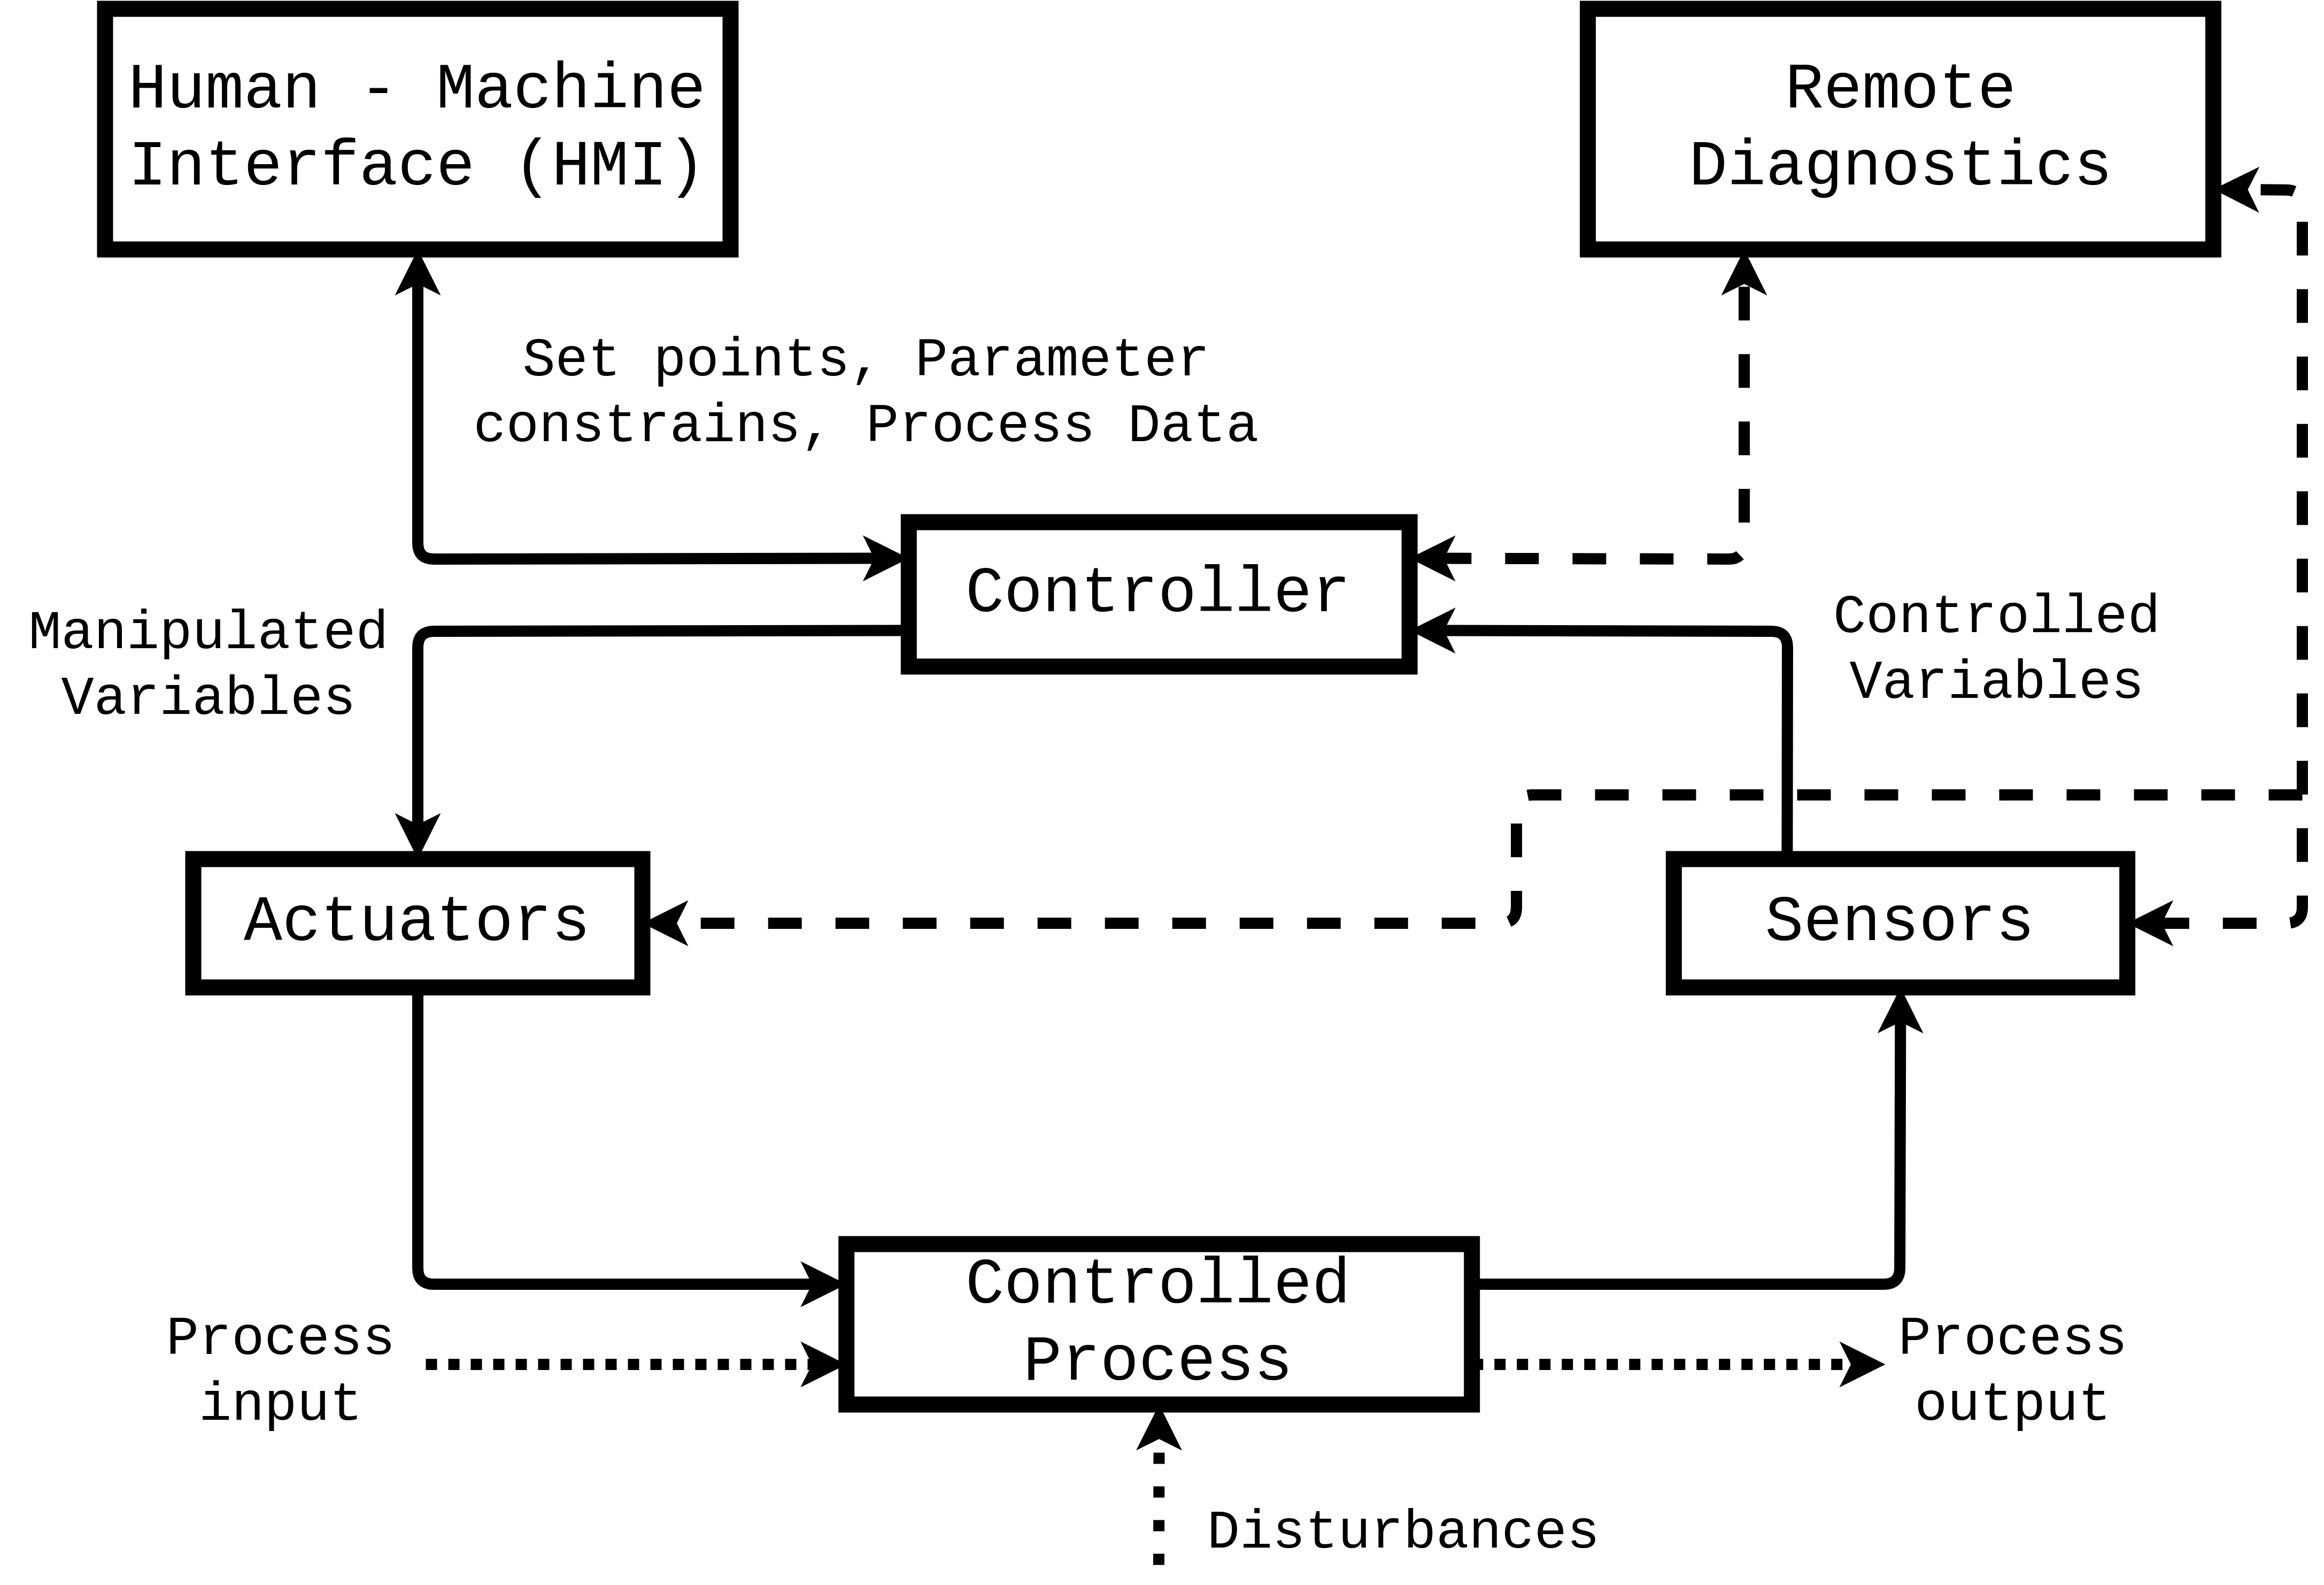
\includegraphics[width=0.8\textwidth]{images/NIST_800.png}
\caption{ICS operation according to NIST, from NIST Special Publication 800-82}
\label{fig:nist_ics}
\end{figure}

Figure \ref{fig:nist_ics} can show an abstract representation of an ICS system. The process in Figure \ref{fig:nist_ics} can be either a small pump process or an entire factory. We can see that the model presented is limited in its applications. 

A more detailed model, made to represent a total view on an ICS deployment, is the Purdue Model \cite{williams1992purdue}. The Purdue Enterprise Reference Architecture, as is its full name, was developed in 1990 by members of the Industry-Purdue University. The model is shown in Figure \ref{fig:perdue}; it gives a hierarchical view of different parts of an ICS system. 

Starting at the bottom with Level 0, we have the devices that form the interface between the physical process and the control system, which are sensors, actuators, and robots, that contain both sensors and actuators. At Level 1, we have different systems of local control, continuous and discrete control of processes and, also the essential safety control. Moving up to Level 2, this is the highest level in what is called a Cell, we have the Human-Machine Interfaces (HMI) and Engineering Workstations. A plant can have more than one Cell. At Level 3, the systems that manage the Cells are located; this is also where the site operations and manufacturing operations systems are. 

Above Level 3 is the Demilitarized Zone (DMZ). This is an area where the critical and sensitive parts connected to the process are separated from the rest of the IT environment of the organization. The DMZ is separated from both sides by firewalls that limit and filter the network traffic that flows in and out of the DMZ. The idea behind the DMZ is to have no direct connection into or out from the Levels 3 and below. If remote access is used in a system, this is where gateways for a remote access system is situated. Level 4 and 5 are where traditional IT resides, email servers, the Intranet, and business planning are located here.

\begin{figure}[h]
\centering
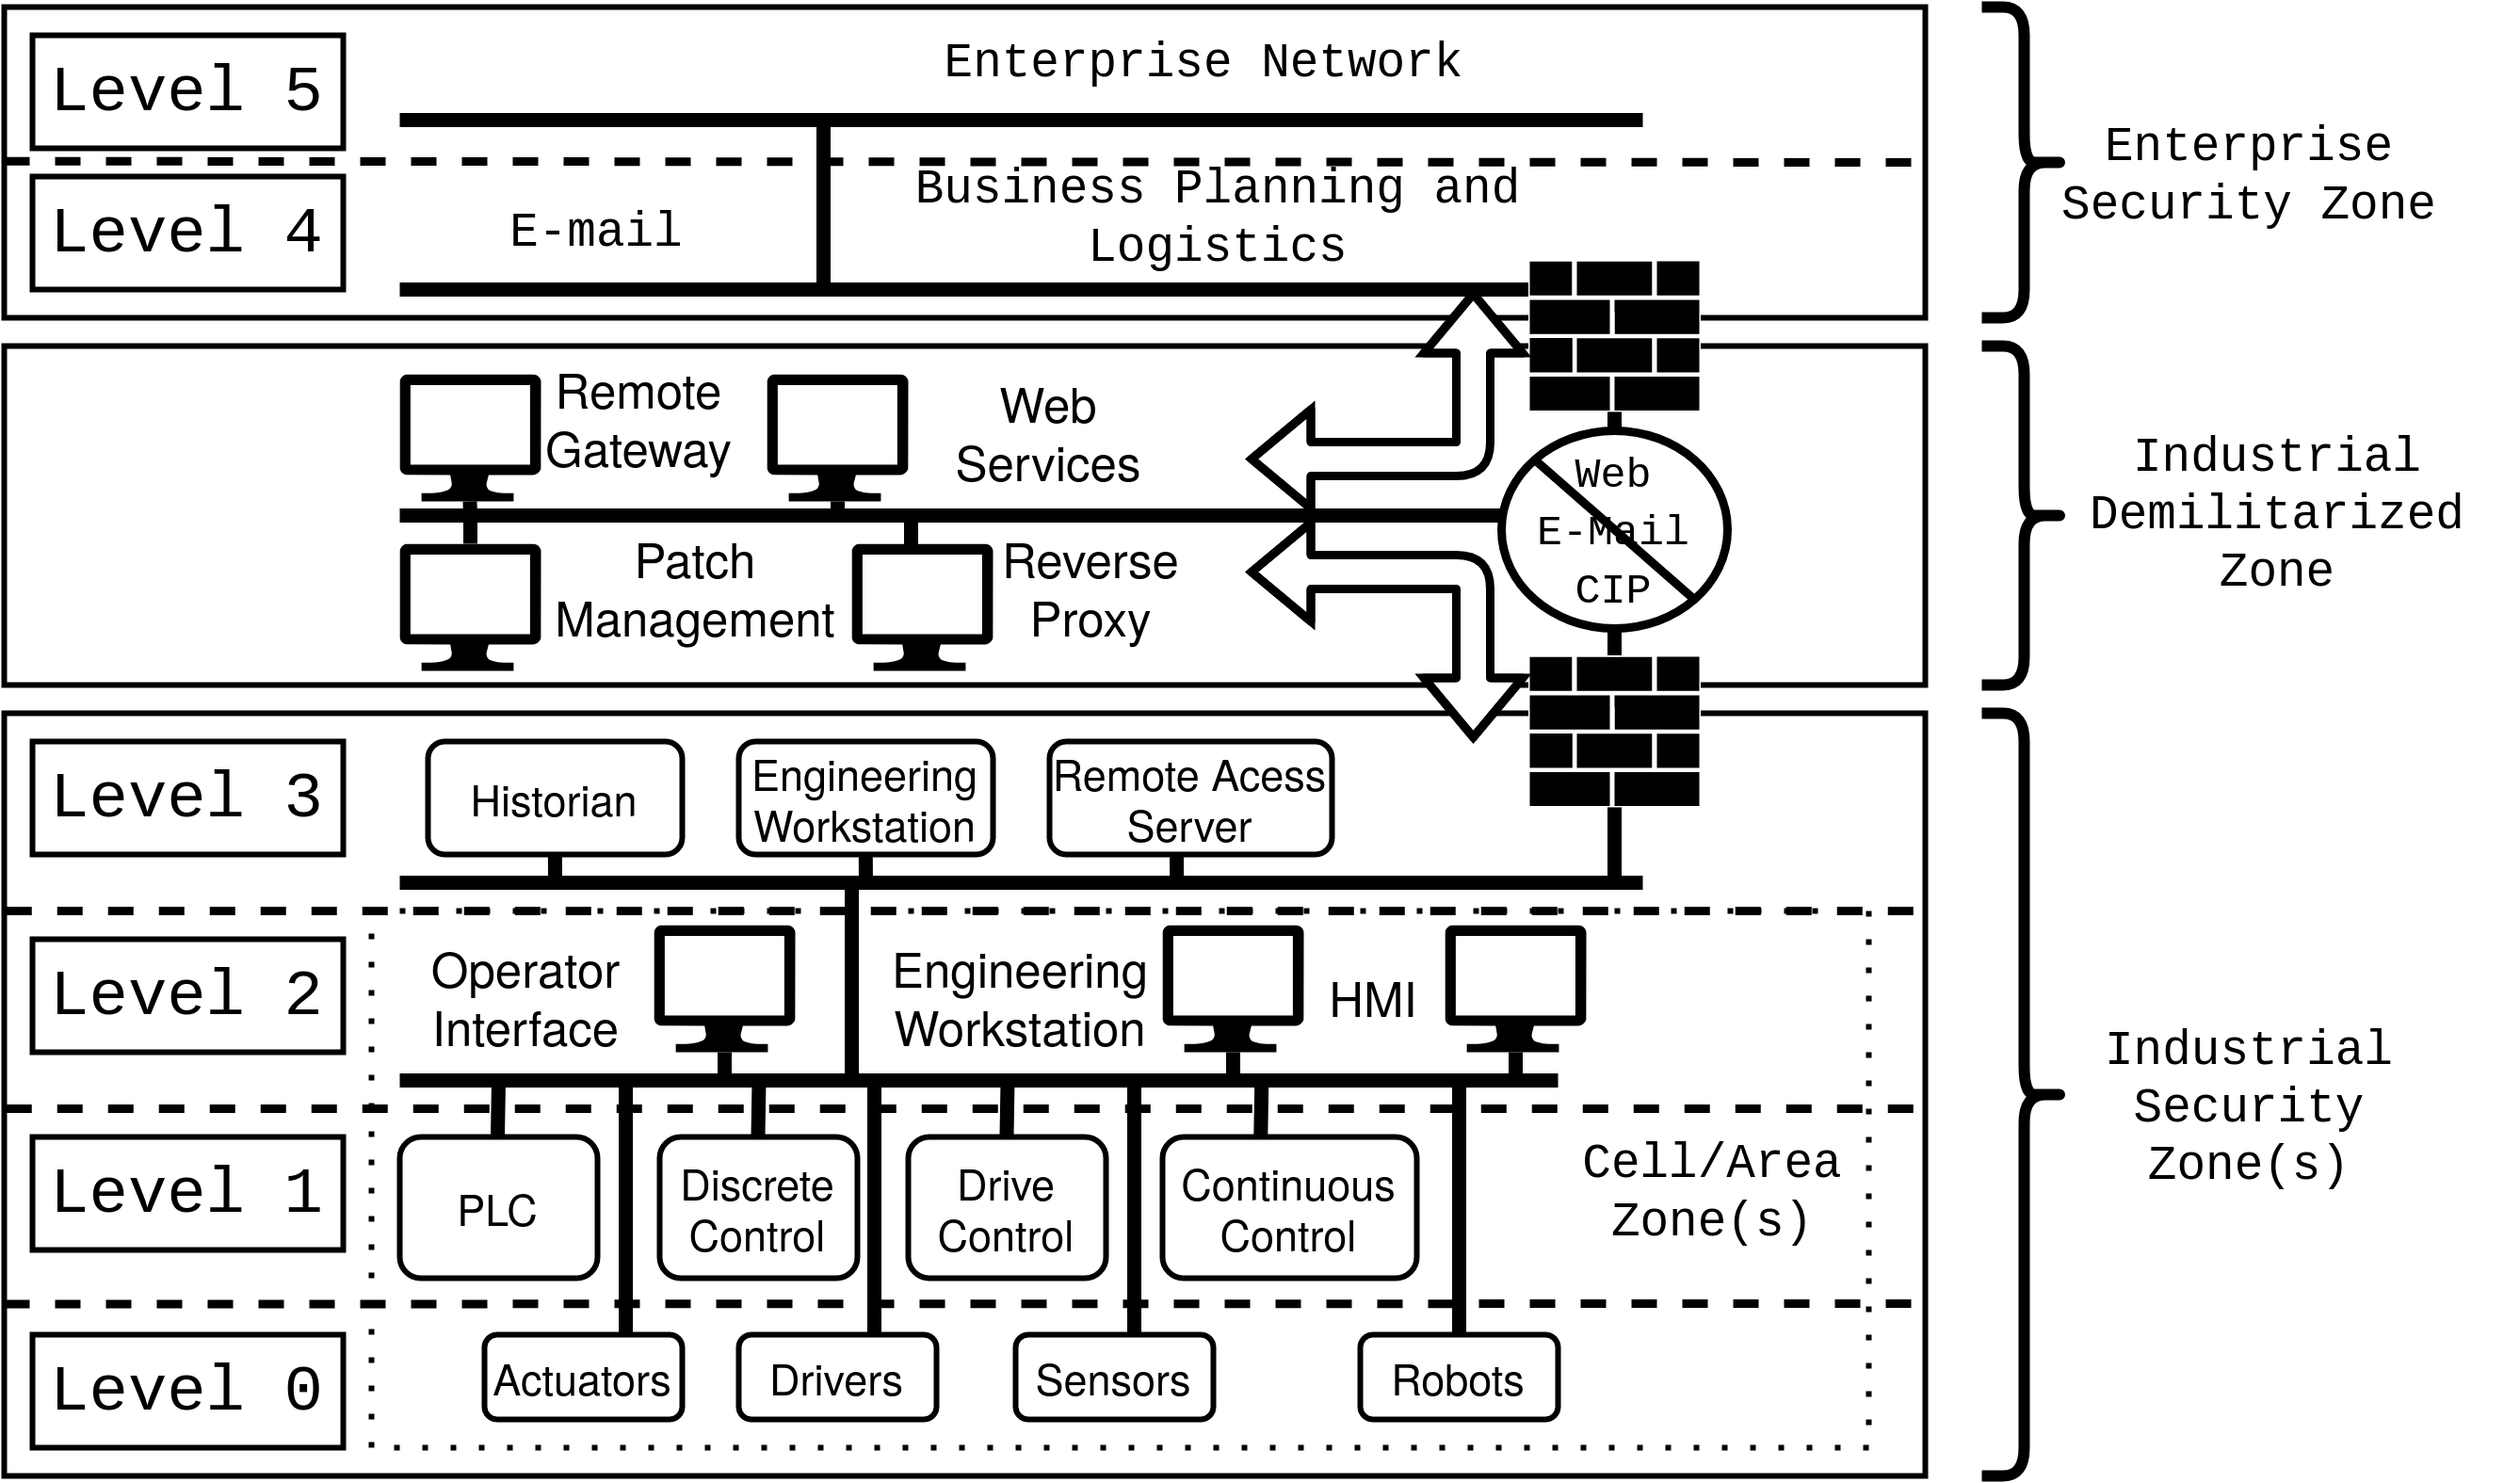
\includegraphics[width=\textwidth]{images/purdue.png}
\caption{The Purdue Enterprise Reference Architecture, a model for ICS.}
\label{fig:perdue}
\end{figure}

Perhaps the most crucial difference between IT and ICS is that in industrial control systems, the \emph{process} is the end goal. The process generate value by producing something, thus it gets prioritized when resources are limited.

Another key technical difference between familiar IT systems and ICS systems is the aspect of real-time tasks in ICS. A process that controls, for example, a chemical process or an electricity grid, cannot have too high latencies. A correct control signal that arrives too late is of no use. In IT, there is often no need for real-time deadlines. Most IT systems process data at the request of a user; as long as the user perceives the system as responsive, the performance is good enough.

Close to the aspect of real-time deadlines is the property of availability; it is easier to have redundancy in an IT system. Multiple instances of a cloud server with a load-balancer can keep a service available even when parts of the system is undergoing maintenance. But in ICS, an outage can have severe consequences, e.g., an electricity grid or freshwater supply, can impact thousands of people. To keep this essential process available; it is important too keep the control system available. The control system is often redundant to prevent outages caused by a faulty control system.


It might, therefore, not come as a surprise that the systems used to control different processes are highly specialized systems. Not only as ICS devices, but also within the field of ICS control systems for different types of processes have significant differences. There is very little commonality between, for example, a welder robot from a car building assembly line and a phase-controller from an electricity grid. The complexity of the process by itself, together with the specialized systems, makes almost all ICS deployments unique.

Because of the specialization of systems, component lifetimes are long. Systems and parts are expensive, a stop in production to install and deploy a system might be too expensive for an organization. Patches are also slowly applied to systems, not only because of the risk of breaking some functionality but also because a certified system might lose the certification when a patch is applied.

Because ICS devices have been developed in silos separated from ordinary IT devices, the protocols, standards, and technologies used in ICS is different compared to a traditional IT environment. This not only affects the interoperability of ICS and IT systems but also does not let ICS systems take advantage of the development of better IT security protocols and mechanisms.

As we have shown here, many aspects differentiate ICS from IT. Of course, these differences impact security, and we will discuss that in Section \ref{subsec:ics_security}.

\subsection{Industry 4.0 and Next-Generation Manufacturing}
\label{subsec:i4}
Sometimes called the fourth industrial revolution, coming after the third Industrial revolution that was the digitalization and computerization of manufacturing from the mid of the 1900s. Industry 4.0 has become the accepted term in Europe on the next generation of the industry.

In 2012 a German research project presented a set of recommendations to the German government about the future of the industry \cite{kagermann2013recommendations}. The goal of \emph{Industrie 4.0} or Industry 4.0 is to improve productivity. The productivity improvements will be gained from an increase in flexibility, where factories build to demand instead of producing to inventory. A critical factor in achieving this will be collecting, sharing, and spreading information through the factory together with decentralized decision making.

The list of technologies and concepts that will realize Industry 4.0 is long; among them are IoT, Cybersecurity, Cloud computing, Big Data, and Simulation. Other technologies are listed, such as Augmented reality and Additive manufacturing, but we will focus on the technologies relevant for this thesis.

IoT is a key component of Industry 4.0, used in this industrial setting Industrial IoT (IIoT) is often used to describe the connected devices in manufacturing systems. In Section \ref{subsec:wsn_iot} we discuss IoT and IIoT. IoT is also key in Paper I, II, and III. 

ICS data collection is needed for advanced analytics and improved production performance, to give two examples. Collecting data from a production environment will often result in large data sets, doing analytics on these big data sets is a whole discipline called Big Data analytics. In Paper II we look at this collecting of data from a privacy perspective. We have identified the 
need for Identity Privacy of data items that is transmitted to a server for analytics.  

 
\subsection{Security Aspects of Industrial Control Systems}
\label{subsec:ics_security}
The properties we have described above make it clear that security for ICS faces different challenges compared to IT security. In IT security, the Confidentiality, Integrity, and Availability (CIA) triad is often used \cite{perrin2008cia} to describe the goals in IT security activities. Note that the CIA refers to the \emph{data} used \emph{in} the system and not the system itself.
The data shall be confidential; that is, it shall not be readable by any unauthorized entity. The data shall be integrity protected, which means that an unauthorized entity shall not be able to manipulate the data. Lastly, the data shall be available since data is of no use if it not readily accessible. 

According to several researchers, for example \cite{Gollmann2016} and \cite{stouffer2011guide}, the CIA security model does not map well to ICS. For example, while the CIA model considers theft or manipulation of data, in ICS risk of human injuries or equipment damage must also be taken into account. See \cite{stouffer2011guide} for a more detailed analysis of this issue.

The availability of systems is more critical in ICS. A production plant can take days to come back online after a stop. The resulting downtime could cause high costs for the owner and operator. 

In this thesis we have included papers that deal both with traditional security properties, like the above mentioned CIA triad, and security life cycle management. Since outages due to maintenance and cyber attacks should be avoided, methods for doing security life cycle management in ICS are needed. It is important that these security life cycle management mechanisms does not consume the limited resources in ICS. In Paper IV we have developed a security architecture using the concept of Digital Twins. Digital Twins are further discussed in Section \ref{sec:digital_twin}, and as shown in the included paper, it is a powerful tool for security monitoring with low impact on legacy system and real-time critical systems.

\section{Constrained Devices}
\label{sec:constrained_devices}
The term \emph{constrained devices} or \emph{constrained nodes} can be used to describe computing devices with limited capability, i.e., they are limited in some way. These limitations can be CPU-Power, RAM and ROM memory, network capabilities such as latency and bandwidth, and energy. Energy can be limited because the device is powered by an energy harvesting device such as a solar panel or from a battery. Devices may sleep for periods of time to save energy and not being able to respond to communication and perform any computation during those intervals.

The Internet Engineering Task Force (IETF) has standardized terminology for these devices \cite{rfc7228}. Because not all constrained devices are the same; IETF has defined several categories that determine \emph{how} limited a device might be. One limiting factor when it comes to performing complex computations; is the size of the available memory. In Table \ref{tab:constrained-classes}, we show the categories of constrained nodes as defined by IETF. Why they use memory instead of a metric such as CPU-speed, is because memory size results in a more substantial factor of the final cost of a device. Memory takes up a lot of space on the semiconductor die, and the size of the die directly influences the price \cite{koopman2015}.


The effect of these memory limitations is that a memory-constrained device is only capable of doing a small set of computations. A small amount of ROM limits the amount of code that can be present in the system, thus only a select few tasks can be done. A small amount of RAM limits the number of intermediary states and the size of the data that can be handled. For example, in a protocol such as Datagram Transport Layer Security (DTLS), RAM limitations directly limits the amount of security contexts which in turn limits the number of simultaneous connection the device can handle.

\begin{table}[h]
\centering
\caption{Classes of constrained devices according to RFC7228.}
\label{tab:constrained-classes}
\begin{tabular}{lll}
\hline\hline
\textbf{Class}  & \textbf{Data Size (RAM)}  & \textbf{Code Size (ROM)}    \\ \hline
Class 0, C0 & \textless{}\textless 10 KiB & \textless{}\textless  100 KiB \\ 
Class 1, C1 & $\sim$10 KiB                & $\sim$100 KiB                 \\ 
Class 2, C2 & $\sim$50 KiB                & $\sim$250 KiB                 \\ \hline\hline
\end{tabular}
\end{table}


Apart from memory constraints, energy is one important aspect to consider when evaluating the capabilities of a system. It is no surprise that running a CPU, peripheral, and a radio-modem consumes energy. Constraints of energy have significant ramifications when a system is designed, energy-efficient CPUs are generally less powerful, and the same goes for peripherals and radio-modems. IETF has put the energy constraints on a scale from 0 to 9, where 9 is no limitation, and 0 is energy harvesting. 

The different categories can be seen in Table \ref{tab:energy-constraints}. For example, an E9 device can be an Ethernet-enabled surveillance camera that is powered by Power over Ethernet. A class E0 device is, for example, an RFID-tag that harvests energy when a reader interrogates it, this small amount of energy harvested is then used to send a reply. 

Since constrained nodes might be sleeping periodically, communication is often asynchronous. The lower layer MAC protocols handle radio duty-cycling and make sure that the receiving node is powered on when it is going to receive messages.


\begin{table}[h]
\centering
\caption{Classes of energy constraints according to RFC7228.}
\label{tab:energy-constraints}
\begin{tabular}{lll}
\hline\hline
\textbf{Class} & \textbf{Type of energy limitation}  & \textbf{Example Power Source}                               \\ \hline
E0    & Event energy-limited                      & Event-based harvesting                             \\ 
E1    & Period energy-limited                     & Periodically recharged battery                   \\ 
E2    & Lifetime energy-limited                   & Non-replaceable primary battery                    \\ 
E9    & No limitations to available energy           & Mains-powered                                      \\ \hline\hline
\end{tabular}
\end{table}

\subsection{Security Aspects for Constrained Devices}
After describing the capabilities and limitations of Constrained devices in the previous section, we will now discuss the implications for security.
Because of the limitation in CPU-power, memory, energy, and network capabilities, traditional security solutions developed for desktop and server computing environments can prove unsuitable. The limited performance of constrained CPUs make public-key encryption time and energy-consuming, hardware-acceleration can be utilized to make it more feasible.

Traditional x509 certificates might require too much bandwidth and memory to be stored in RAM in a device. Research has been done to reduce these numbers \cite{forsby2017lightweight}, but also with limited network capability; it might be difficult to validate an entire certificate chain, thus severely limiting the usefulness of certificates.

The ubiquitous protocol for secure communication in traditional IT Transport Layer Security (TLS) \cite{RFC8446} uses TCP as the underlying transport mechanism. Sessions are not desirable when constrained devices communicate asynchronously. Instead, DTLS is standardized as an alternative to TLS. DTLS uses UDP as the underlying transport; this removes the need for TCP sessions. Using UDP also reduces the overhead of each transmitted packet.

The security protocols and solutions developed for constrained devices must take these limitations into consideration \cite{I-D.irtf-t2trg-iot-seccons}. Security solutions must be resource-efficient. Limiting message overhead to save bandwidth and energy is a requirement. When selecting cryptographic primitives, efficient algorithms must be prioritized. This means using symmetric-key encryption where it is possible and limiting the use of public-key cryptography. Reducing the transmitted message size is also an important goal since transmitting and receiving data consume energy. The protocol OSCORE, recently standardized by IETF, was designed with low message overhead as one of the design goals \cite{RFC8613}. We have evaluated the efficiency of the OSCORE protocol in Paper III; we investigate message overhead and energy consumption to examine the efficiency of the protocol. 

In Paper I, we have developed a Secure ownership transfer protocol for very constrained devices. The protocol we have designed uses symmetric cryptography and results in an efficient protocol. The topic of Secure ownership transfer will be described in detail in Section \ref{sec:ot}. In Paper II, we have designed a protocol that gives Identity privacy for sensor data; the protocol is designed using Object security principles. Object security and identity privacy is described in Section \ref{sec:object_security}. This protocol is also using symmetric cryptography to achieve the stated efficiency requirements. 

\subsection{Wireless Sensor Networks and Internet of Things}
\label{subsec:wsn_iot}
Wireless sensor networks are a designation for a network of, often constrained, devices that communicates with wireless technology. The purpose of the network is often to collect sensor readings from several different places and collect the data for further processing in a central server. 
The shrinking of processors and the decrease in the price of micro-controllers and associated devices have made it possible to deploy sensors with a micro-controller and some kind of networking capability very cheaply. Often these systems are powered by a battery, combined with the need to keep costs down the resulting systems can usually be classified as Constrained devices, as described in Section \ref{sec:constrained_devices}. 

Internet of Things has become the catch-all term for all kinds of connected devices. Everything from a factory connected to a SCADA network to a refrigerator with WiFi can be called an IoT device. Sometimes distinctions are made such as Industrial IoT (IIoT) for connected devices used in an industrial setting. The difference between IIoT and the connected control systems described in Section \ref{sec:cps} is that IIoT is more connected to computing resources such as a cloud environment \cite{mclaughlin2016undiscovered}. An IIoT deployment will differentiate from the Purdue reference model we showed in Figure \ref{fig:perdue} in that an IIoT deployment will have a direct connection between the edge devices and the cloud. There is no DMZ in IIoT, like the one that can be found in the Purdue model.


\begin{figure}[h]
\centering
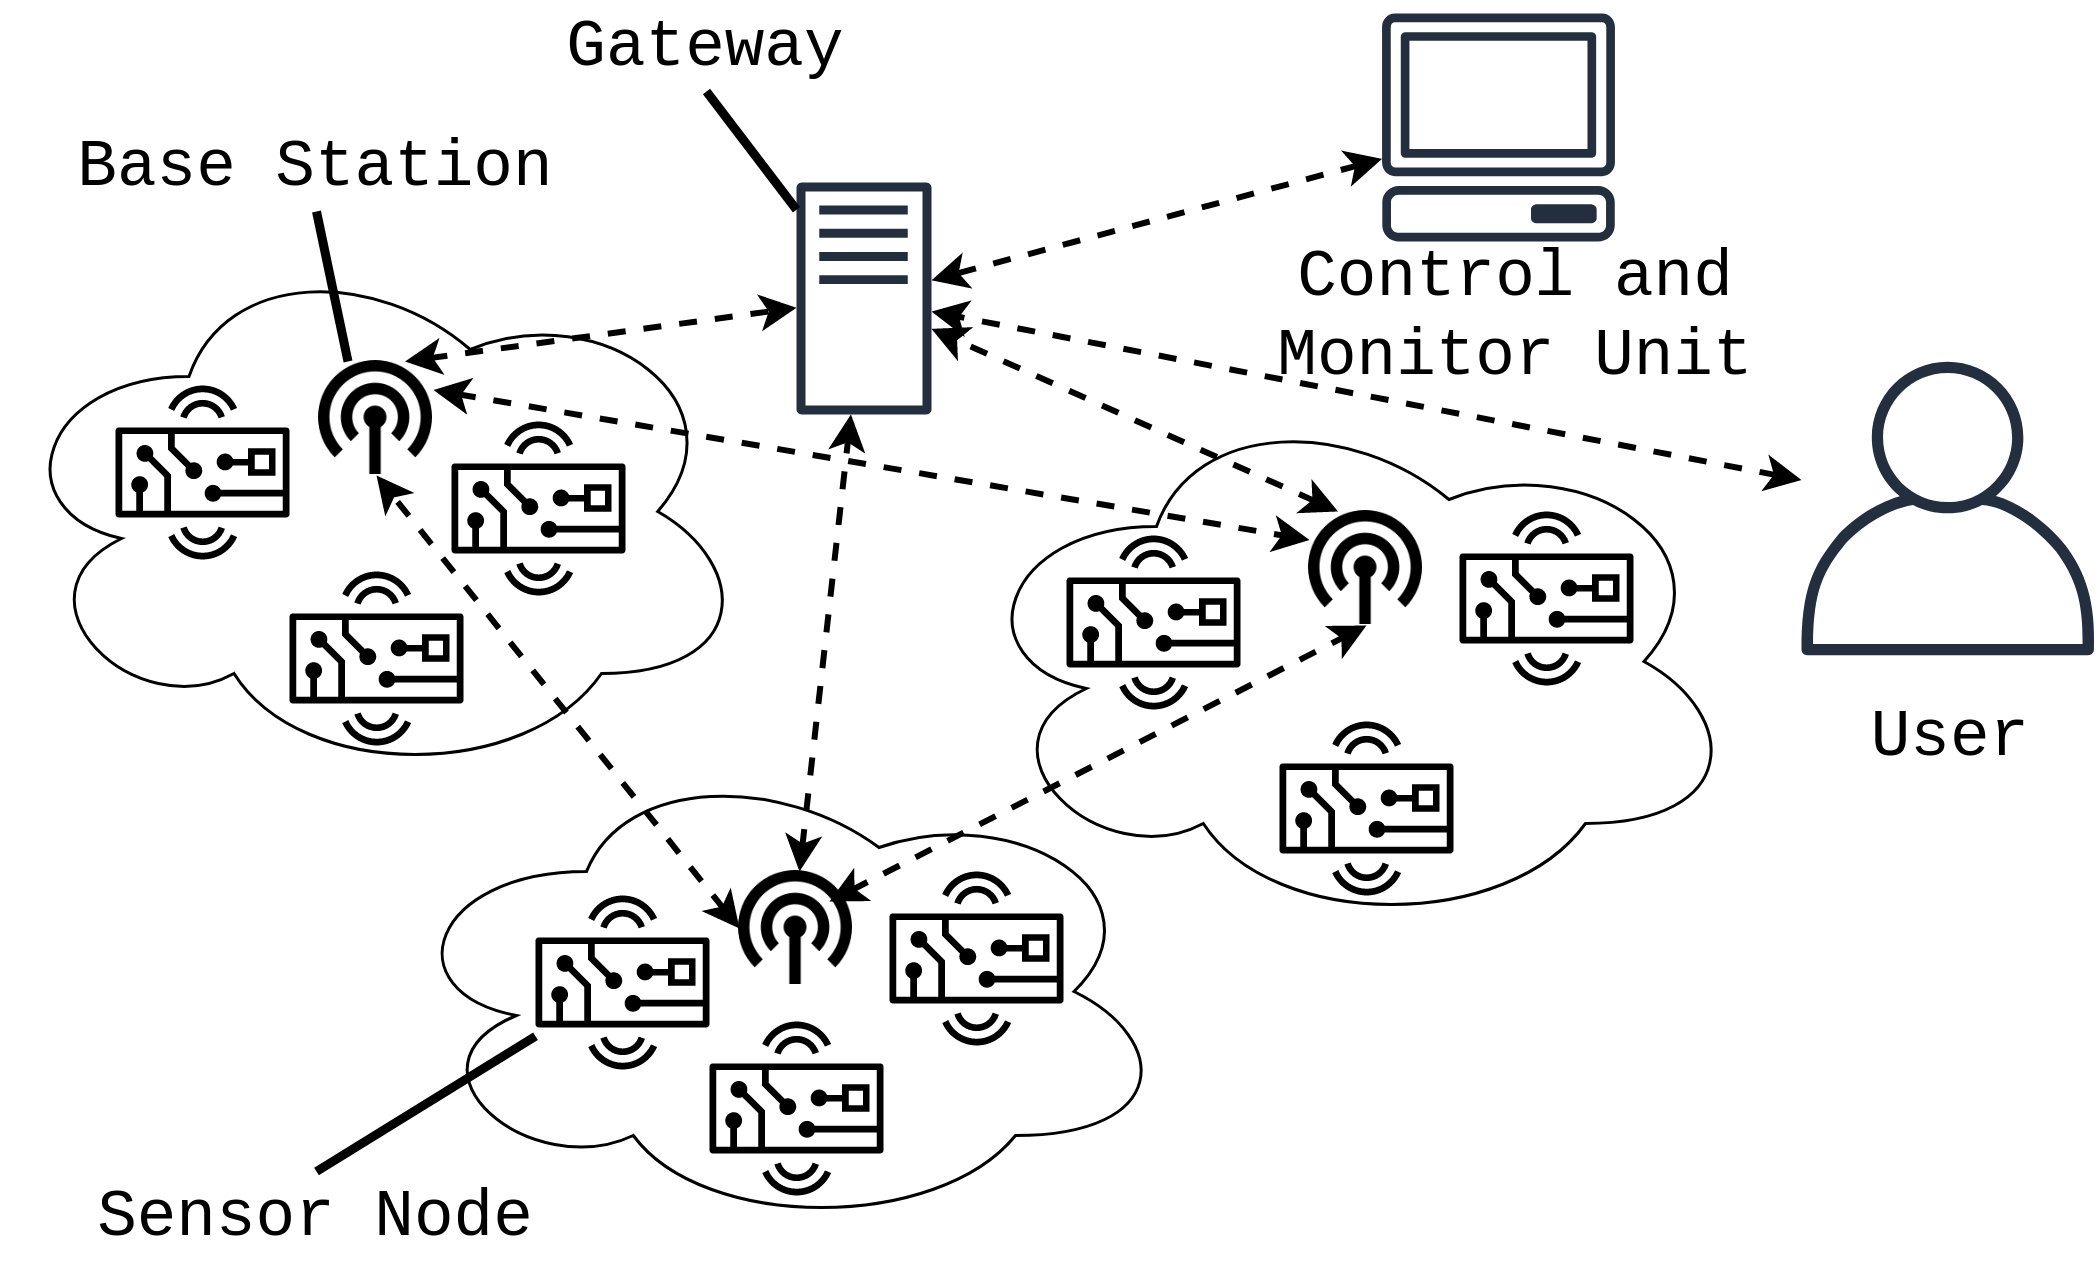
\includegraphics[width=0.9\textwidth]{images/WSN.png}
\caption{A schematic of a Wireless Sensor Network in an industrial setting.}
\label{fig:wsn}
\end{figure}

\subsubsection{Communications Standard for Wireless Sensor Networks}
Many actors have developed Wireless Sensor Networks; as a result of this, there exists a large number of communication protocols and network stacks. WiFi, Bluetooth \cite{haartsen2000bluetooth}, Bluetooth Low Energy (BTLE) \cite{heydon2012bluetooth} and Zigbee \cite{alliance2010zigbee} all use the unlicensed 2.4 GHz frequency band. LoRA \cite{sornin2015lora} uses unlicensed frequencies in the sub-gigahertz range to increase the range compared to the protocols in the 2.4 GHz band. NB-IoT\cite{ratasuk2016nb} uses optimized cellular technology and base stations to achieve wide coverage.


Several communications protocols exist, the two most common is MQ Telemetry Transport (MQTT) \cite{hunkeler2008mqtt} and Constrained Application Protocol (CoAP) \cite{rfc7252}. MQTT is of type publish-subscribe; clients subscribe to topics, and publishers publish data to these topics. Message brokers then act as intermediaries to forward the data from the publishers to the relevant subscribers.
MQTT is usually transmitted over Transmission Control Protocol (TCP), and TLS is used to secure TLS connections and, in extension, MQTT.
CoAP is a RESTful protocol like Hypertext Transfer Protocol (HTTP). It is transmitted over User Datagram Protocol (UDP), and the most common way of securing it is with DTLS. In this thesis, we have evaluated OSCORE, an alternative approach to securing CoAP. OSCORE uses a security concept called object security that we introduce in Section \ref{sec:object_security}.

\section{Object Security}
\label{sec:object_security}
The earliest reference to Object Security was made in 1995 in RFC1848 \cite{RFC1848} titled \textit{MIME Object Security Services}. The document details how Multipurpose Internet Mail Extensions (MIME) objects shall be encrypted and processed. MIME is a standard that relates to email. Encrypting each mail in a self-contained object is good solution. The sender can not know if the recipient is able to receive the email at the time of sending, this means that setting up a secure session to the recipient does not work. The problem with the recipient not being available at the time of sending is solved by using intermediate servers that store and forward the emails. Protecting each mail in a self-contained object eliminates the need for secure sessions between the intermediate servers.

One schematic diagram of an object security message can be seen in Figure \ref{fig:object-security}. It does not show any actual message format, but rather a sample of some fields that might be present in such a structure. What differs between formats and standards, not shown in the figure, is encoding. 

\begin{figure}[h]
\centering

\includegraphics[width=0.9\textwidth]{images/object_security.pdf}
\caption{A schematic of a message or data item protected with object security.}
\label{fig:object-security}
\end{figure}


Object security is a good fit for when a device sends messages to several receivers. Sending is only done at intervals. Thus object security eliminates the need for keeping a session alive. 
Apart from email, wireless senor networks and constrained networked devices have proved a good fit for object security. Because of the energy limitations and constrained nature of devices, messages are only sent sporadically.

Object security has also been used in web contexts, such as JavaScript Object Notation (JSON) Web Signatures (JWS)\cite{jones2015json}, JavaScript Object Signing and Encryption (JOSE)\cite{barnes2014use} also XML encryption\cite{imamura2013xml}. A similar standard to JOSE is CBOR Object Signing and Encryption (COSE)\cite{schaad2017cbor}.  CBOR stands for Concise Binary Object Representation and has been standardized by IETF as a more compact alternative to JSON\cite{rfc7049}. The difference between JOSE and COSE is the encoding, JOSE uses JSON while COSE uses CBOR. Due to the compact serialized format of CBOR, COSE is more compact than JSON \cite{kalvoda2015implementace}.

One benefit of the object security concept is that it can be used to provide end-to-end encryption. If a message takes a winding route to its destination, encrypting the message in a self-contained way is a practical solution to protect the contents until it arrives at the destination. This is why PGP and all other email encryption schemes work so well; encrypted email can travel between many email-servers until they arrive at the receiver. The receiver, provided they possess the correct keys, can then decrypt the message. These schemes and protocols are quite old now, but they are still used in email applications today. 

Perhaps the first implementation of object security for a constrained wireless device can be found in \cite{brown2000pgp} were the authors port Pretty Good Privacy (PGP) to a Research In Motion (RIM) pager. The RIM pager has more memory than a Class 2 constrained device, but it is still a relatively limited device, considering it uses a 10 MHz Intel 386 CPU from the 1990s. In the paper, they find that Elliptic curve cryptography (ECC) can be done in a couple of seconds. Elliptic curve cryptography is a type of public-key algorithms that require smaller keys and less computation than alternative algorithms for a given level of security. These qualities make ECC suitable for use in constrained devices. The authors argue that the performance of ECC can be acceptable for an email solution.

One more recent application for object security is end-to-end security for instant messaging apps. Asynchronous communication make this method of securing messages a good solution. The person you send a message to might not have a direct connection to you, so instead of setting up a secure channel, encrypting the message in a self-contained way and sending it through intermediaries that do not possess the key provide end-to-end security for the message. 

This use-case is very similar to the problem statement behind OSCORE. Messages pass through intermediate proxies and middle-boxes, the receiving server might be sleeping to preserve energy. Because of this, setting up a secure session is not desirable since a client would have to wait until the sever wakes up.  

Even if object security can solve some security issues, one issue that remains is identity privacy. A message to a receiver like a message shown in Figure \ref{fig:object-security} can have the origin revealed by the Key ID. A server that receives messages from many sources must be able to choose the correct key to decrypt messages. To enable the server to select the right key for decryption, there must be a readable Key Identifier. However, a malicious entity can also read this Key Identifier. Since symmetric keys are shared between only a single pair of communicating entities, knowing the Key ID and the receiver, knowing the sender is trivial. 

This is a privacy problem, if a malicious adversary can learn what messages originate at a particular device or person, learning that specific entity's patterns become likely, for some application, this might not be a problem. In others however, it might reveal patterns about the originating device. Information might be deduced from encrypted messages, even if the contents of which are not known, by analyzing when messages are sent and where they originates. One possible solution to this would be to encrypt either the entire message or just the Key ID with the recipient's public key. Doing that, only the intended recipient can decrypt the message. Using public-key cryptography might, however, be too resource-intensive for some devices.

\section{Secure Ownership Transfer}
\label{sec:ot}
Secure ownership transfer is the process of transferring the control of a secure system from one entity to another. The general premise is that each device has some kind of key or credentials; these keys and credentials are shared with the owner. Some kind of server usually represents the owner. Here we will stick to using \emph{key} for any such credential.

The process of transferring the keys from the old owner to the new is not a suitable solution. The terms \emph{New owner privacy} and \emph{Old owner privacy} have been used to describe desirable features \cite{taqieddin2018tag}. Old owner privacy is that the new owner shall not be able to decrypt recorded traffic and access data from the old owner. New owner privacy is that the old owner shall not be able to learn secrets from the new owner after the transfer is complete.

The topic of ownership transfer has been studied both for IoT and networked devices but more intensively for RFID-tags. RFID-tags are a relevant problem because RFID-tags attached to things, such as parcels, change hands, and move around. RFID-tags can be read remotely in close proximity of the tag; this has raised privacy issues. In \cite{juels2006rfid}, the author describes a scenario were RFID-tags carried on a person can be read to reveal sensitive information about their owner. Using keys to enable authorization of RFID-tag access and encryption of the data in transmission, has been proposed as a solution to this privacy issue. 

When items with RFID-tags that use keys to authorize reading and provide encryption of the transmitted data change hands, the new owner must be able to access the RFID-tag after the transfer. Ownership transfer is the name given to this problem. The first publication that tries to solve this problem was \cite{saito2005reassignment}. 
Several approaches for ownership transfer exists, protocols have been proposed for single tag transfer or multiple tag transfer. There are also another aspect of proposed solutions, with protocols including a trusted third-party and protocols only involving the old and new owner. 

A schematic view of RFID deployment and ownership transfer can be seen in Figure \ref{fig:rfid-ot}. One crucial property for RFID-tags is that they are only powered on when they are read, i.e. interrogated. The RFID-tag reader is an essential part of the system since that is the only device that can directly read the RFID-tags. The RFID-tag reader is usually able to do more advanced computation and is not usually limited in energy. Thus it can be used in the system to perform more complicated computation.

\begin{figure}[h]
\centering
%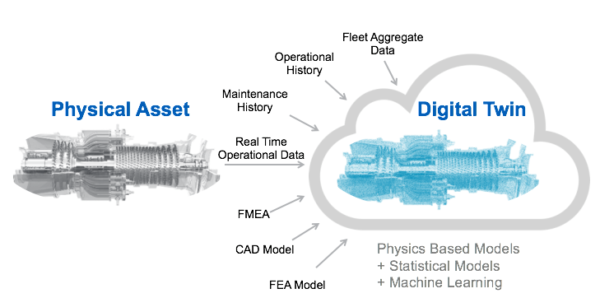
\includegraphics[width=0.9\textwidth]{images/digitial-twin.png}
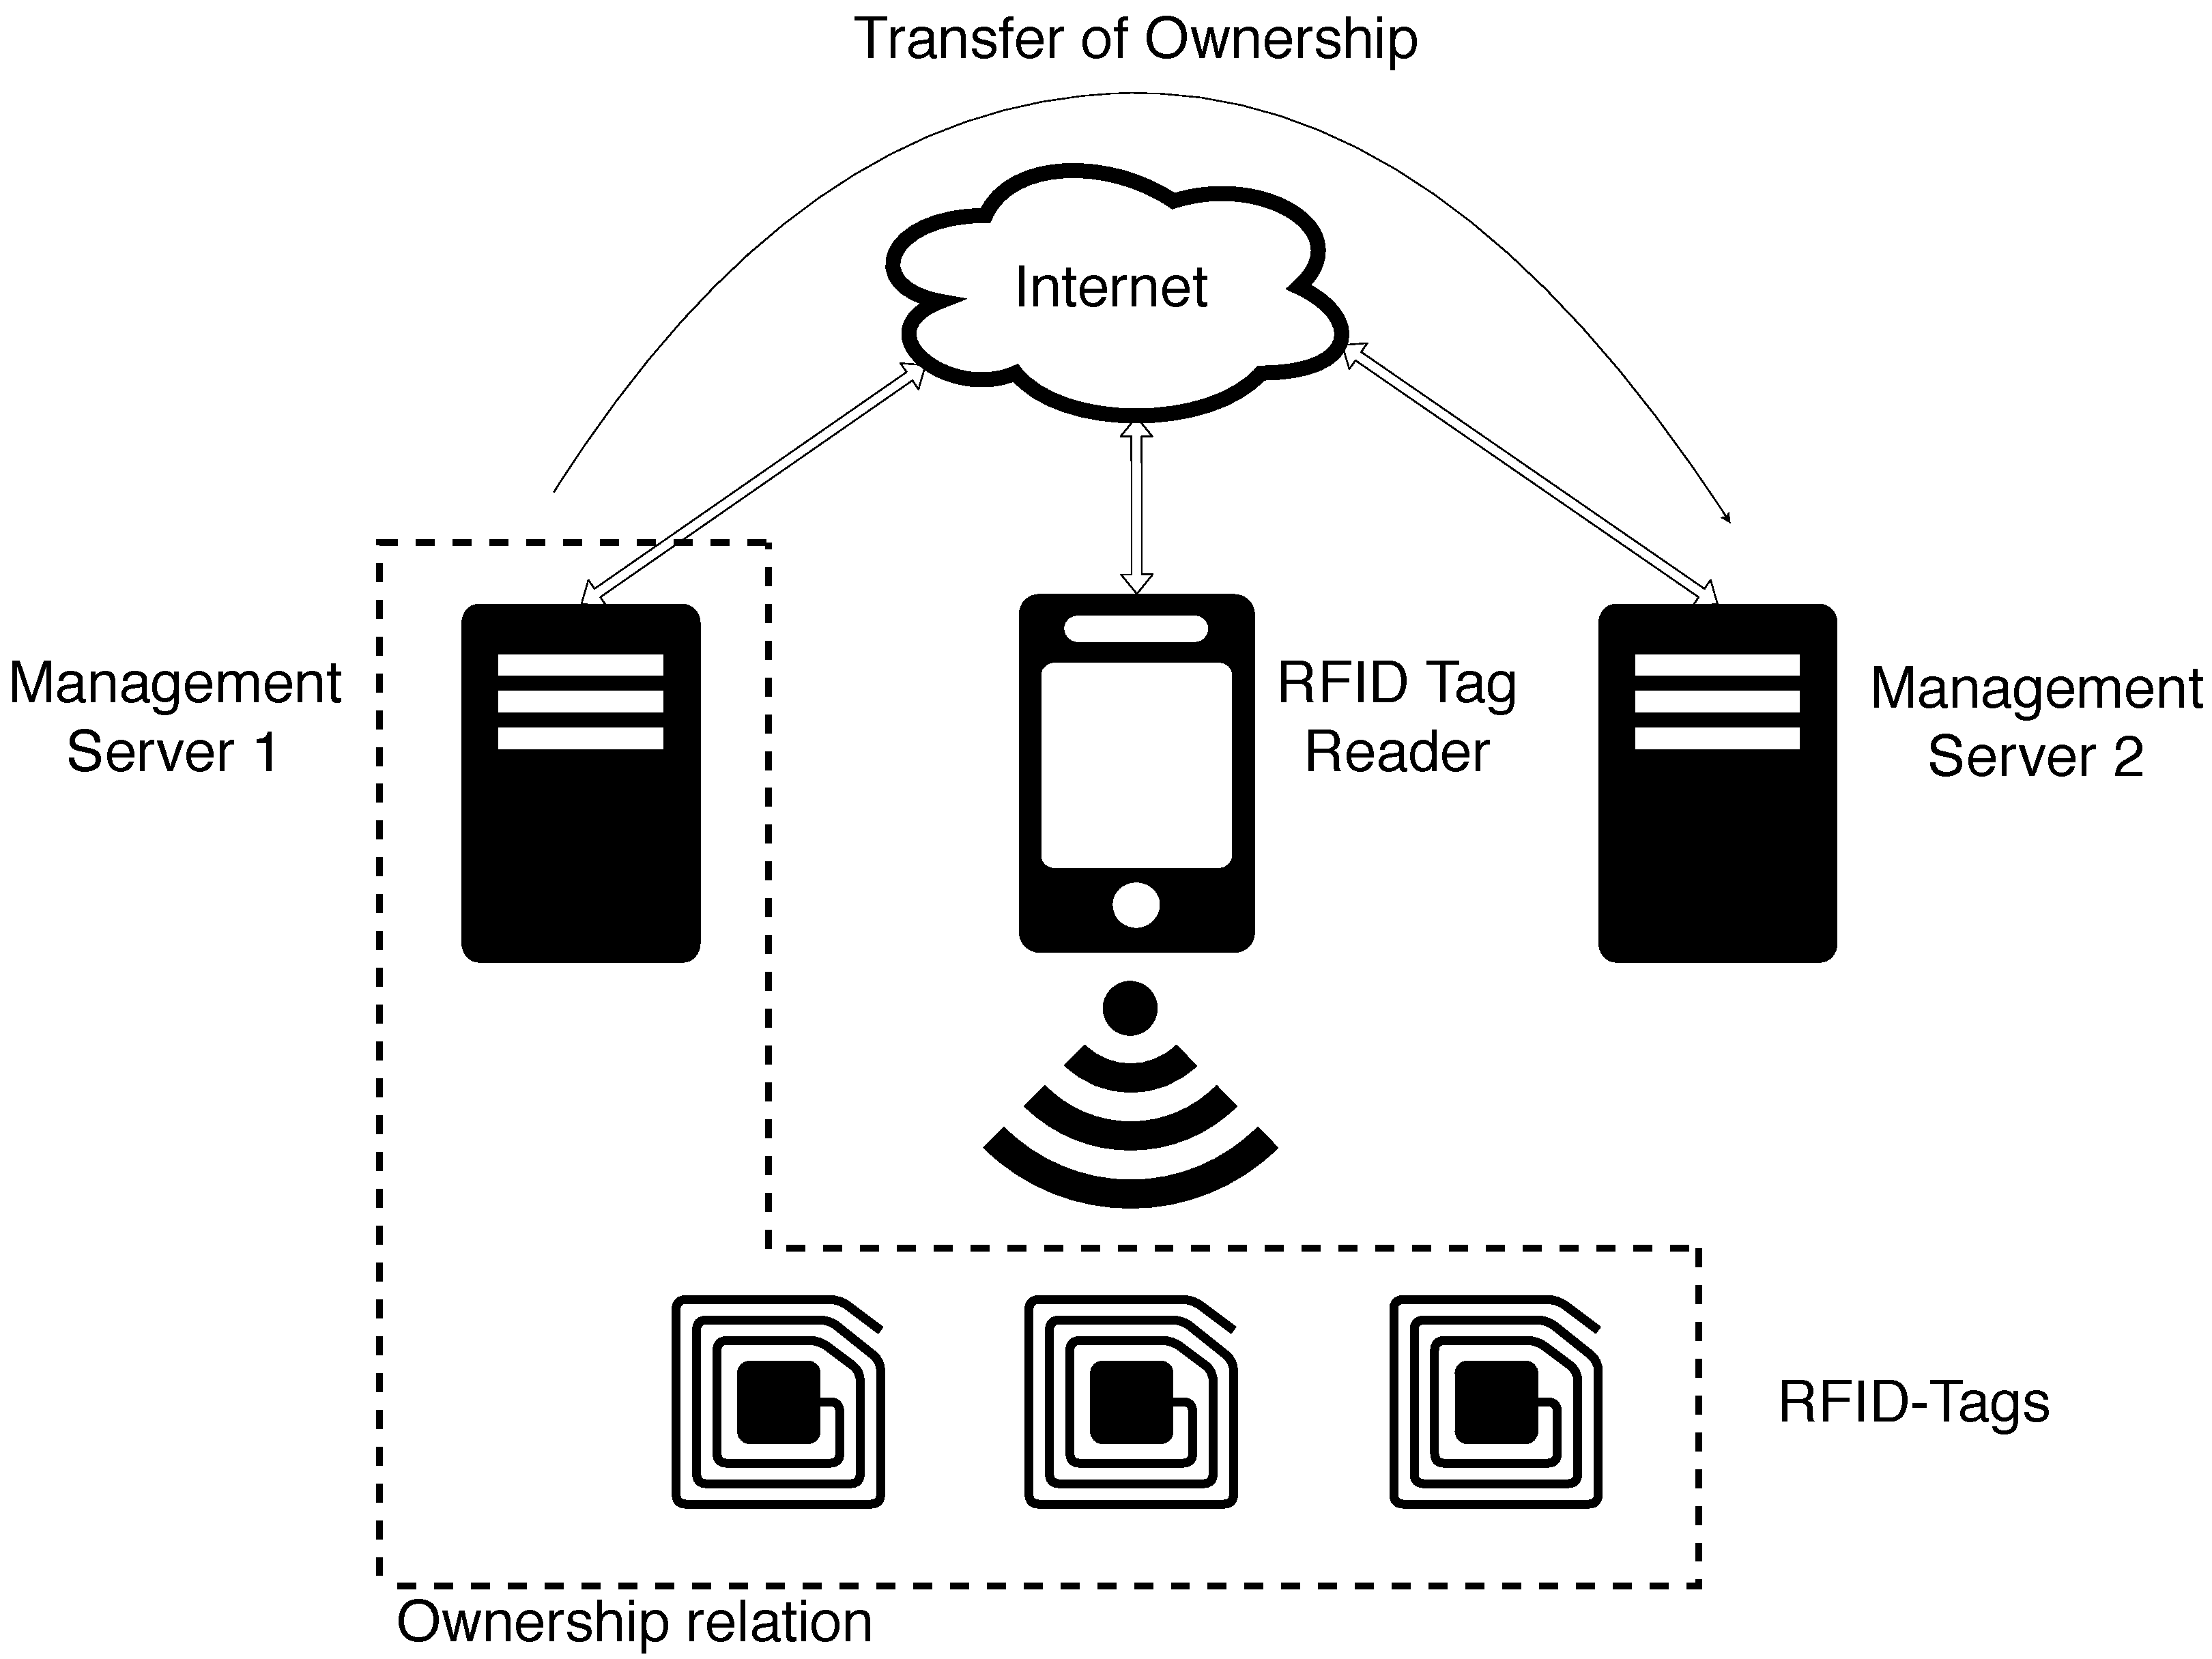
\includegraphics[width=0.9\textwidth]{images/RFID-Tag_OT.pdf}
\caption{RFID-System and ownership transfer}
\label{fig:rfid-ot}
\end{figure}



A recent and comprehensive survey of the research into ownership transfer can be found in \cite{taqieddin2018tag}.
Some ownership transfer solutions for IoT \cite{tam2004protocol}, use public-key encryption to solve this problem in a straightforward way. However, constrained systems might not be able to handle the complex computations needed for public-key encryption. Besides the computational issue, not all devices might have the memory needed to store the necessary keys and the code needed to do public-key computations.

In Figure \ref{fig:iot-ot}, we show a schematic overview of an IoT deployment. The Management server does not directly connect to the individual devices, but often communicate over the internet, through some gateway. The presence of the gateway is an essential property of such a system. This gateway sometimes need to translate protocols and terminate DTLS sessions to work correctly. Since individual IoT devices are connected to the Internet, the attack surface is larger compared to an RFID tag. An attacker must be in proximity to an RFID-tag to be able to communicate with it and to intercept messages. Thus many of the security requirements for RFID-systems can not be directly applied to IoT systems.


\begin{figure}[h]
\centering
%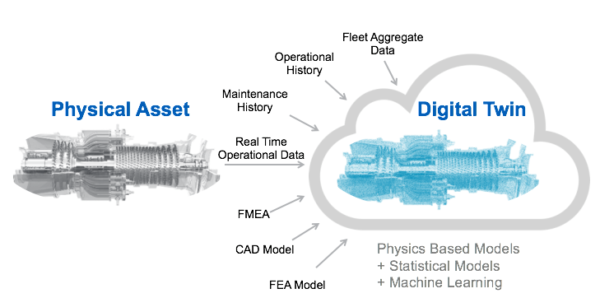
\includegraphics[width=0.9\textwidth]{images/digitial-twin.png}
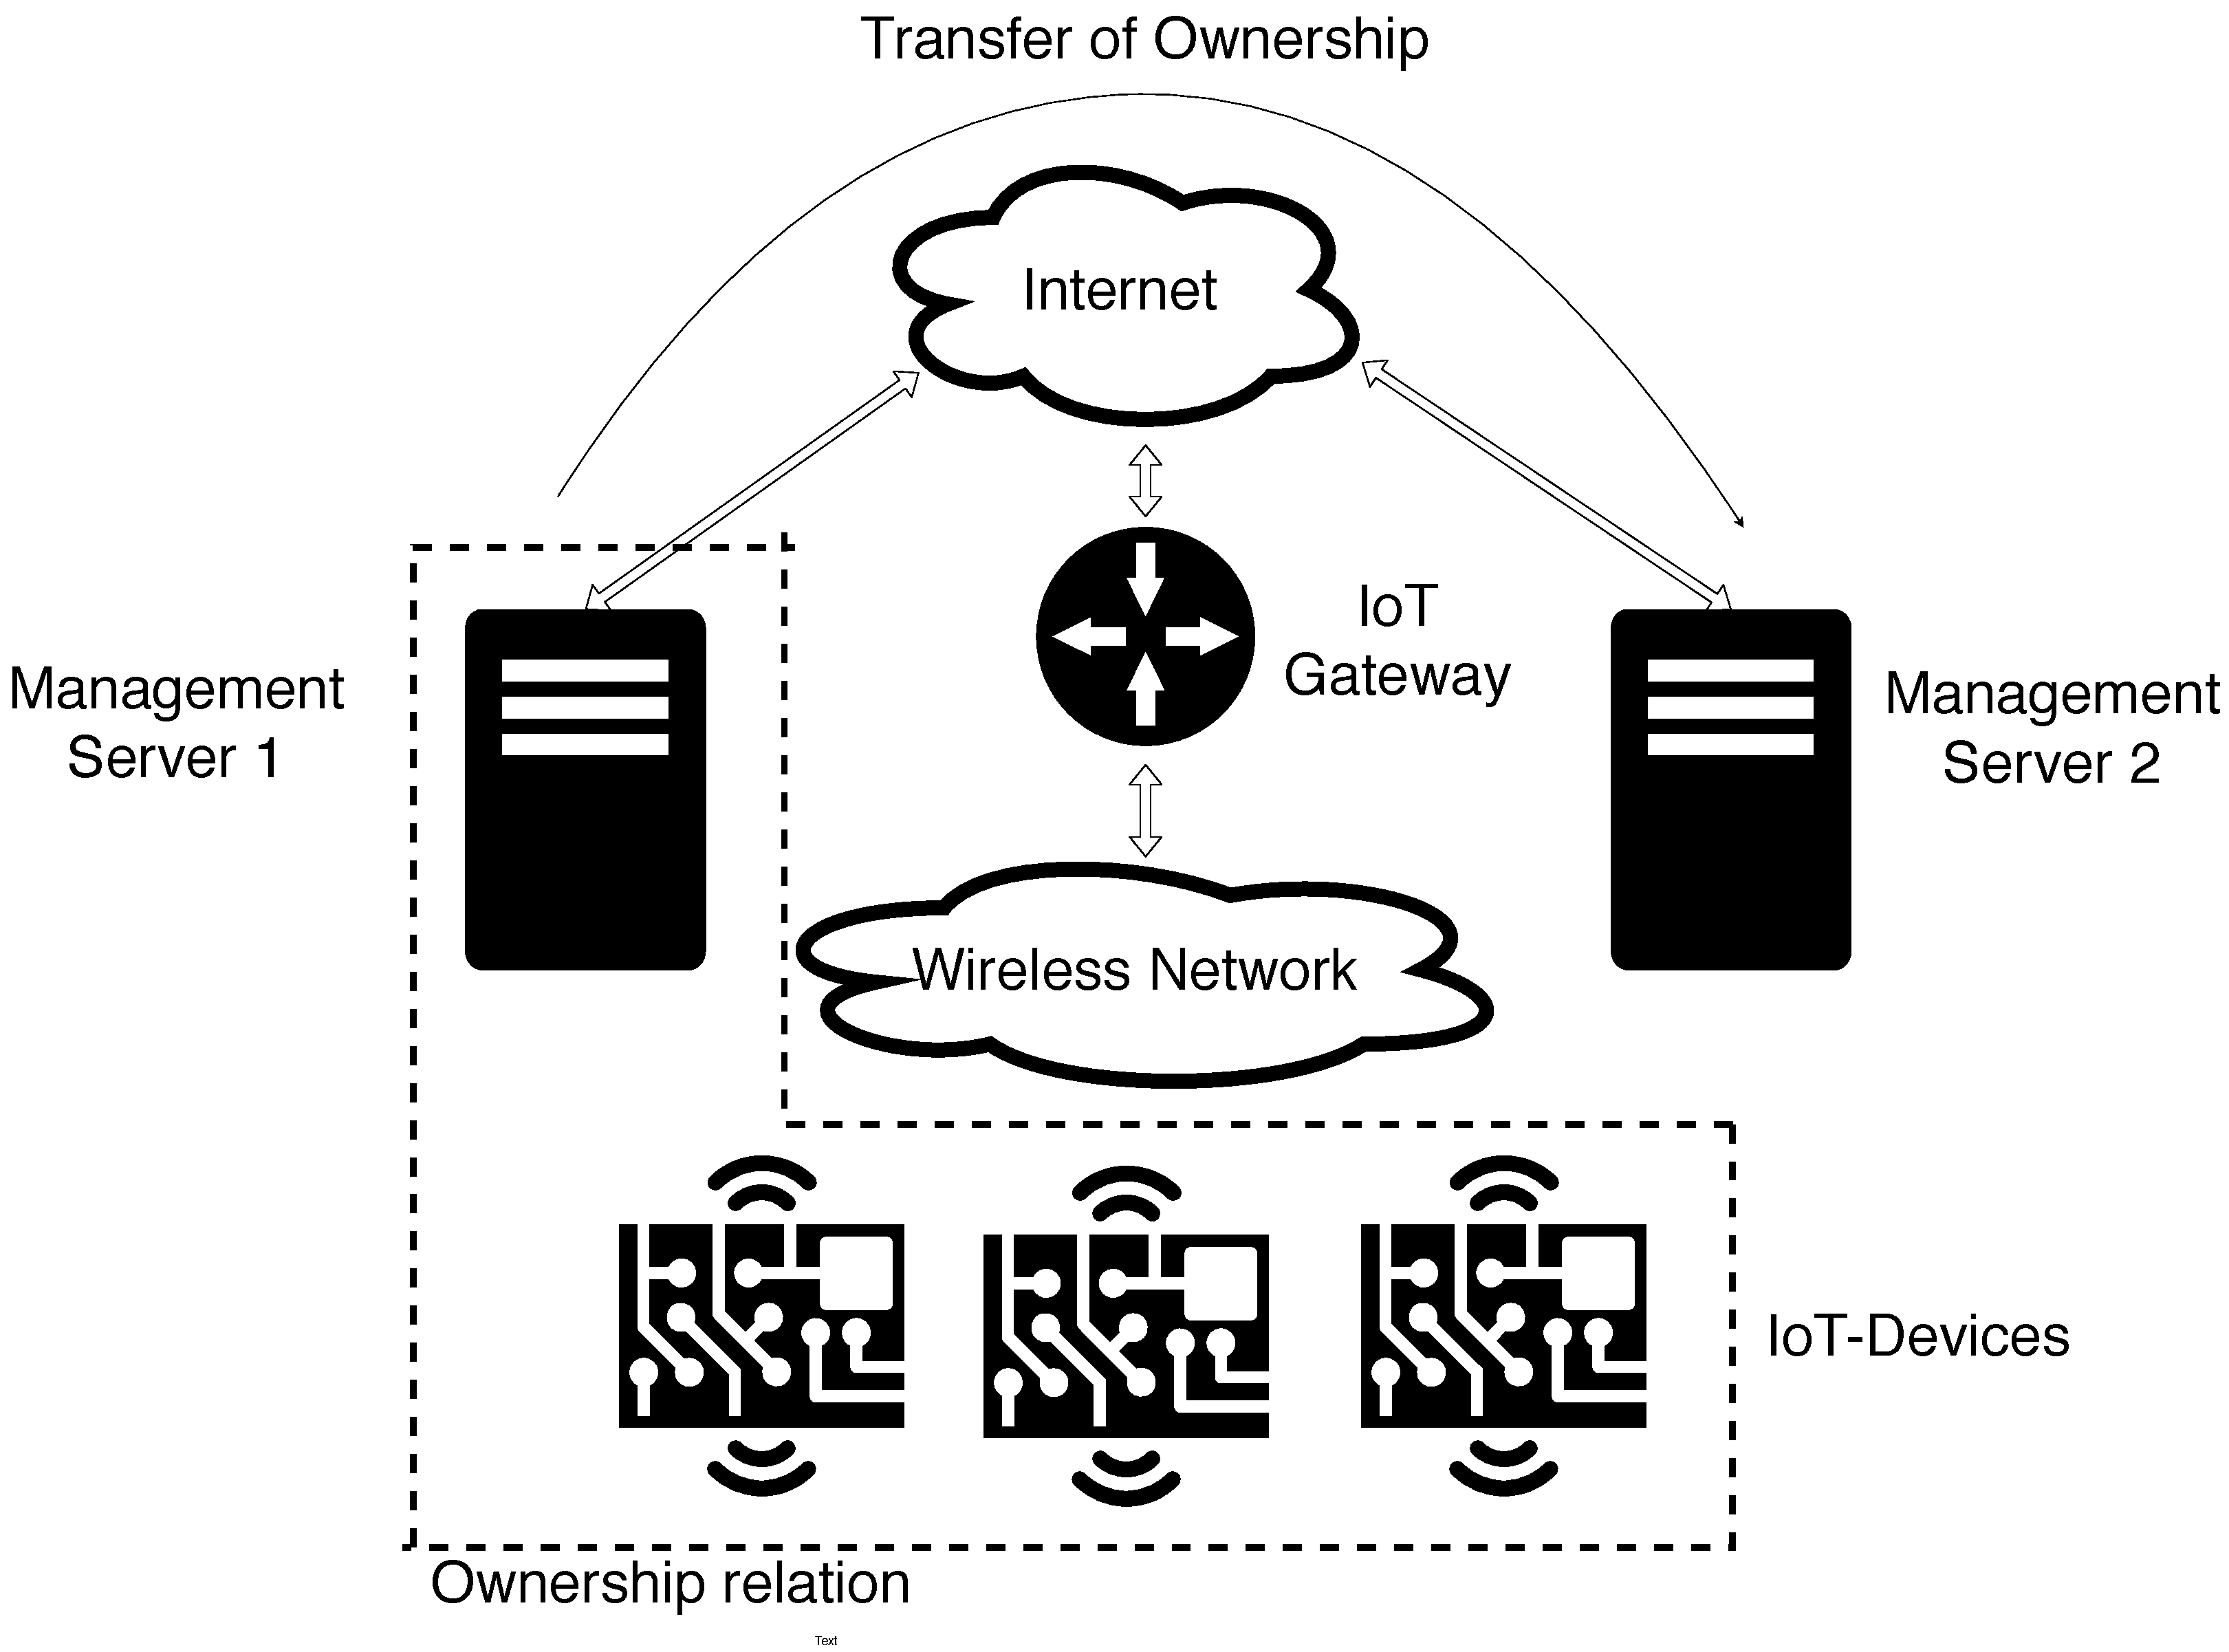
\includegraphics[width=0.9\textwidth]{images/IoT_OT.pdf}
\caption{IoT deployment and ownership transfer}
\label{fig:iot-ot}
\end{figure}


Security requirements for secure ownership transfer protocols are the same as for conventional security protocols. Properties such as confidentiality, integrity protection, availability, and resistance to impersonation attacks are essential to a secure protocol. But then there are new properties that need to be also considered. According to \cite{taqieddin2018tag}, the authors have proposed the security requirements stated below. These requirements apply equally to both RFID-tag solutions and IoT protocols since they are general to the problem of ownership transfer:
\begin{itemize}
    \item New owner privacy: The old owner shall not be able to access data after ownership transfer is completed.
    \item Old owner privacy: The new owner shall be unable to learn anything that the old owner has done before the transfer.
    \item Windowing problem: There shall be no place in time where both the new and the old owner has access to the device at the same time.
    \item Exclusive ownership transfer: It shall possible to verify that the ownership transfer has gone according to plan.
\end{itemize}
The properties of New owner privacy and Old owner privacy is similar to Forward Security and Backwards Security in a protocol such as TLS. For example, TLS ephemeral keys are negotiated with a key agreement protocol such as Diffie-Hellman \cite{diffie1976new}. Using such a solution work in theory for ownership transfer, but it fails when considering the computational complexity of public-key cryptography. Achieving New owner privacy and Old owner privacy using symmetric cryptography is the challenge here. 

The Windowing problem means that the transfer must be immediate, so there can be no point in time where both the New owner and the Old owner have access to the device that is switching hands. The challenge here is not apparent; when the step that transfers the ownership occurs, it will either succeed or fail. If it completes, then the New owner will have control of the device, but if it fails, the Old owner shall retain control of the device. This has to be done to prevent the device from becoming \emph{orphaned} and left in a state where neither the New owner or the Old owner can access it. 
Exclusive ownership transfer means that the New owner shall be able to verify that devices have been transferred and that they are now under the New owner's control. The requirement here is that the New owner must be able to authenticate all devices after a transfer has been done.

%\cite{RAY2018838}


\section{Digital Twin}
\label{sec:digital_twin}
 Digital Twin is the name given to techniques where a physical device is \emph{mirrored} to a digital copy. This Digital Twin can then be used to perform computations, such as optimizations that can be implemented on the \emph{physical} twin. Several definitions of the term exist, "A digital twin is a real-time digital replica of a physical device" is a succinct definition from \cite{bacchiega2019}. Digital Twin as a concept has its origin in aviation manufacturing, where aircraft engines were one of the first applications. The concept was developed during the 1990s and was published in 2002 \cite{grieves2019virtually}. Since then, the application of Digital Twin has spread to Wind Turbines, HVAC (Building Automation), health applications, and many more. 

In Figure \ref{fig:digital-twin}, we show how such a workflow with continuous improvements can look. The concept of continuous simulation has been studied by academia \cite{boschert2016digital}.

In \cite{grieves2014digital}\cite{grieves2017digital}, the authors present their idea of how to use Digital Twin to facilitate life-cycle management for complex systems. They discuss how to test, simulate, and improve the physical systems using the digital Twin. But this is not the only application; many industries and fields investigate what benefits they can get from Digital twin. A summary of these results can be found in \cite{8424832}. 

\begin{figure}[h]
\centering
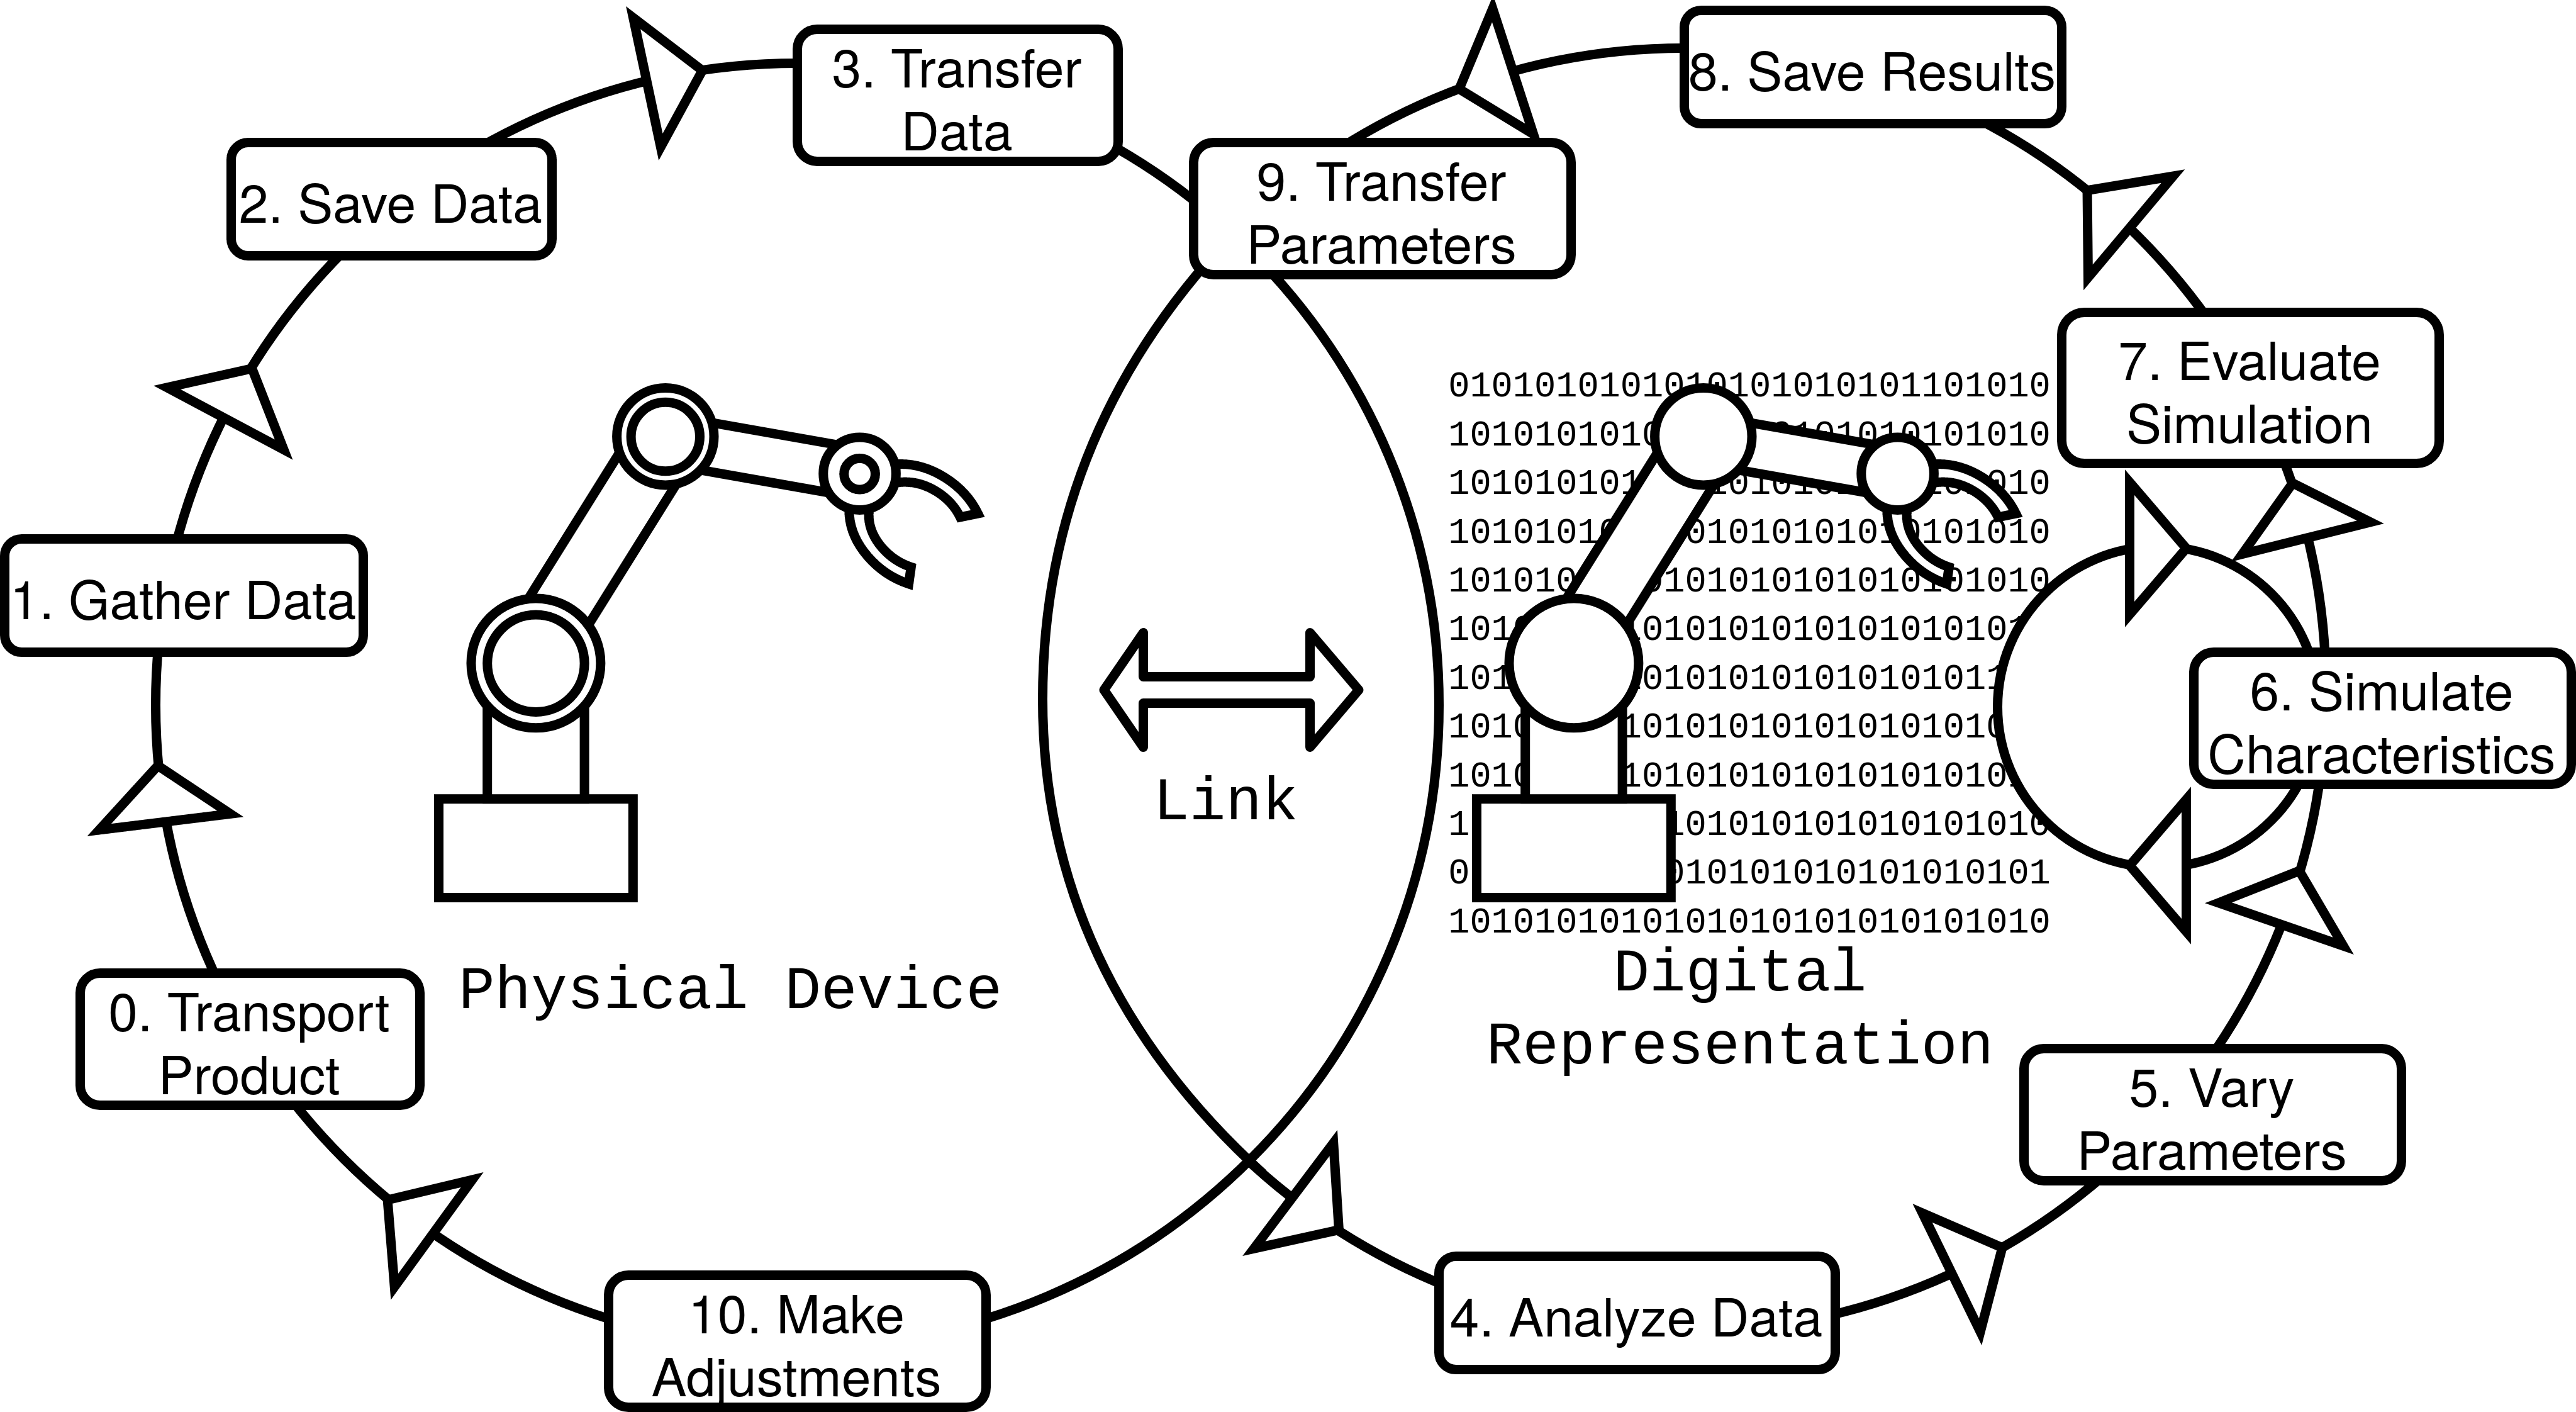
\includegraphics[width=\textwidth]{images/digital_twin.png}
\caption{One of the many ideas of a Digital twin. (Picture should be redrawn)}
\label{fig:digital-twin}
\end{figure}

Digital Twin can also be used to improve security. In heterogeneous systems, it can be challenging to establish a picture of the system. A Digital Twin of the system can provide such a picture. This twin can be used for finding vulnerabilities, both by scanning for known vulnerabilities, static threat modeling and also to create a replica of the system to be used in a \textit{Cyber Range}. 

ICS systems are often so vulnerable to a cyberattack that techniques used in penetration testing such as port scanning can cause systems to crash. Since these systems are connected to a process, a crash is unacceptable, but stopping the process to do a penetration test is usually not possible either. If this penetration test can be made on a \emph{twin} of the system, it would solve both these problems. 

In \cite{bitton2018deriving}, the authors provide a way to generate a digital twin of a system that can be used in a penetration test. The Digital Twin can also be used in a cyber range to teach operators of ICS about cyber security applied to \emph{their} system.

Digital Twin has been proposed to be useful for many things, such as documentation and continuous improvement. For cybersecurity in Industrial control systems and Constrained devices, the ability to synchronize the physical device to a Digital Twin can be used to overcome the limitations we described in Section \ref{sec:cps} and \ref{sec:constrained_devices}.

The ability to replicate a state from a device to a remote entity makes it possible to add functionality to the remote entity. This entity can be a cloud environment, and with a state replication protocol, the results of this added security functionality can be \emph{mirrored} to the physical device. We have investigated such a concept in Paper IV, where we propose a simple state synchronization protocol for use in Industrial control systems.

\subsection{State Machine Replication}
Finite-state machines can be used for representing and modeling a variety of computer and automation systems. State machines can also be used to design and specify the behavior of a system. State Machine Replication is a technique to synchronize the states between two or more Finite-state machines \cite{lamport1984using}. 

It might also come as no surprise that computers and automation systems sometimes fail. Adding redundancy to provide fault-tolerance is one way to overcome the problem. By viewing a part of the system as a state machine and then replicating the state to another part of the system, one can achieve redundancy and reducing the probability of a system-wide outage. 


\begin{figure}[h]
\centering
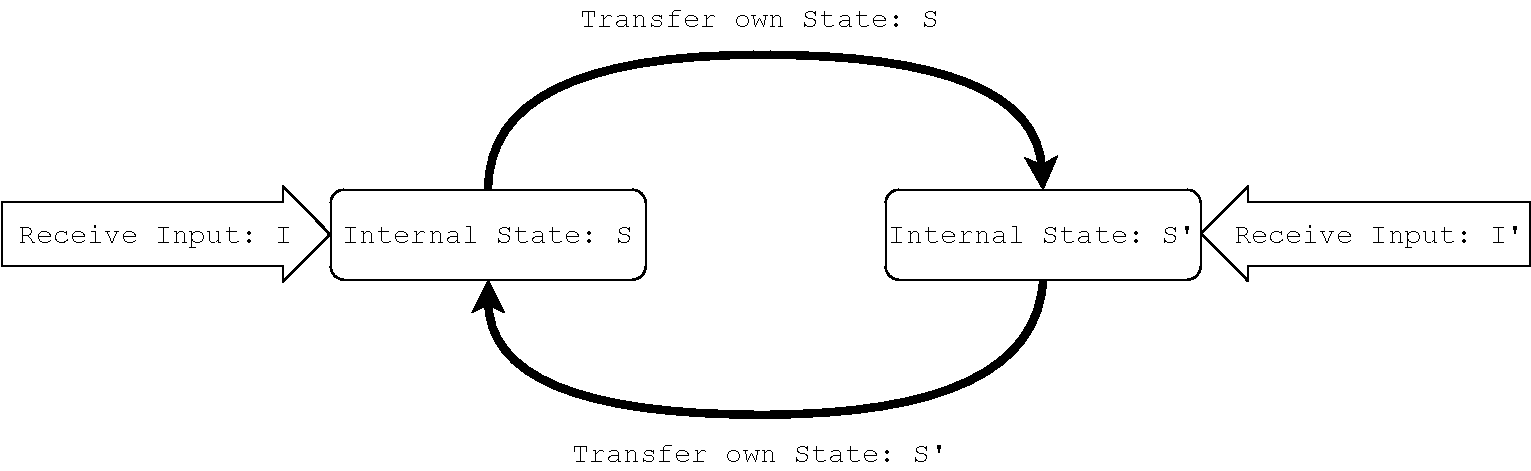
\includegraphics[width=0.9\textwidth]{images/State_replication.pdf}
\caption{A conceptual model of a state replication mechanism}
\label{fig:state-replication}
\end{figure}

As can be read in \cite{charron2010replication}, Replication and State Machine Replication have been investigated for over 30 years. The techniques have been applied to different fields, such as distributed systems and databases. The goal of replication has been both performance, by scaling a system and fault tolerance, by duplication of stored data. By mirroring a physical system with a digital twin, a new type of application emerges. Here the goal is to provide a single digital image of a system that can be used for further processing.

Above, Digital Twin was defined as: "... a real-time digital replica of a physical device", State machine synchronization is one way of achieving \emph{real-time replication}.

Using replication to improve the security of IoT devices has been suggested in \cite{gehrmann2016iot}. The authors present a method to \emph{mirror} an IoT device to a server. The server can provide more extensive security mechanisms than the constrained IoT device. By using a rigid communications protocol that only allows for synchronization between the device and the mirror, a high level of security can be achieved for a constrained device.

The technique of state machine replication has been applied to Industrial Control Systems. In \cite{Eckhart2018}, the authors propose a state replication mechanism to be used for intrusion detection in ICS. The authors use a state replication approach to avoid prohibitive overhead in terms of network and computation overhead in the physical devices.

\begin{figure}[h]
\centering
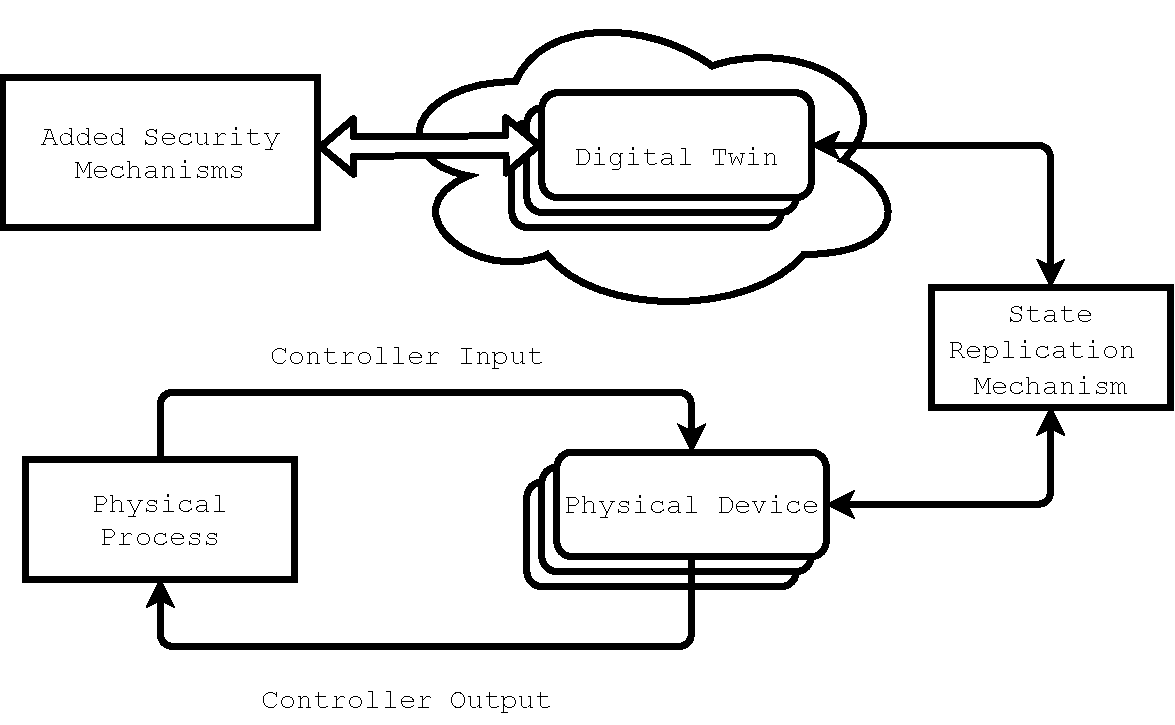
\includegraphics[width=0.9\textwidth]{images/state_replication_security.pdf}
\caption{Adding security mechanism by replicating the physical devices to Digital twin and perform the complex security mechanisms there.}
\label{fig:state-replication-sec}
\end{figure}

Both \cite{gehrmann2016iot} and \cite{Eckhart2018} propose a similar approach to adding more complex security mechanisms to constrained devices and Industrial Control Systems. In Figure \ref{fig:state-replication-sec}, we show a system overview of such a solution. For constrained devices, this type of solution is attractive because of the limitations in the capabilities we discussed in Section \ref{sec:constrained_devices}. A state synchronization protocol can be implemented with small overhead, so this approach is workable. For ICS, the limitations in available resources that we discussed in Section \ref{sec:cps}, the long lifetimes of devices in ICS, and the complexity of these devices can benefit from the added security mechanisms with the relatively low cost of implementing a State Replication Protocol.

In Paper IV we have used a State machine synchronization protocol to synchronize a physical device with a Digital Twin. The low overhead of a state machine synchronization protocol makes this an attractive solution to realize a Digital Twin for ICS, considering the limitations described in Section \ref{sec:cps}.

\chapter{Contributions and Conclusions}
\label{ch:coc}
\section{Contributions}
The following sections introduce each contribution, the individual contributions of the author, and the changes made to the publications for print in this thesis.

Author names and acronyms; Martin Gunnarsson (MG), Christian Gehrmann (CG), Joakim Brorsson (JB), Marco Tilcoa (MT), Ludwig Seitz (LS), Francesca Palombini (FP).

%1 OT, 2 Big Data, 3 OSCORE, 4 DT
\subsection{\paperItitle}
\subsubsection{Content}
In this paper, we investigate the problem of Secure ownership transfer. The process of transferring ownership of devices has mainly been studied for RFID-tags but not for IoT devices. The core problem with ownership transfer is \emph{New owner privacy} and \emph{Old owner privacy}. This means that after the transfer of ownership, the new owner shall be unable to learn anything that has happened on the device or any message sent. The old owner shall not learn anything the new owner does after the transfer. 
The work that has been done on Secure ownership transfer for IoT has focused on solutions using public-key cryptography. 
In our intended system, the devices we consider for ownership transfer are Constrained devices, as described in Section \ref{sec:constrained_devices}. Because of the limitations in performance, we have developed a Secure ownership transfer protocol using symmetric-key cryptography.
\subsubsection{Individual Contribution}
MG has together with CG, designed the Secure ownership transfer protocol. CG stated security requirements and, together with MG, did the security analysis of the protocol. MG did the Tamarin model and formal verification of the protocol. MG implemented the experimental evaluation and produced the experimental results.
\subsubsection{For this Thesis}
The paper has been formatted to match the rest of this thesis.


\subsection{\paperIItitle}
\subsubsection{Content}
Wireless sensor networks are being deployed in larger numbers. The data that is sampled is usually sent to a remote server for analytics. This server might be owned by a third party or running in a cloud environment. This is a scenario envisioned in both Industry 4.0 and Industrial IoT, as described in Sections \ref{subsec:i4} and \ref{subsec:wsn_iot}.

Collecting and analyzing data in such a way can provide increase efficiency. However, sending data can reveal secrets about the origin of the data, being either individuals or company secrets in an industrial setting. To solve this privacy problem, we propose a new scheme of identity-privacy for data items. We have described the problem of readable Key Identifiers in Section \ref{sec:object_security}. Our proposed scheme only uses symmetric key operations and is suitable for very constrained sensors of the type we described in Section \ref{sec:constrained_devices}. The proposed protocol uses the concept Object Security, that we detailed in Section \ref{sec:object_security}, and encrypts each data item individually. These data items can then be stored intermittently in an encrypted form without extra processing.
\subsubsection{Individual Contribution}
CG designed the protocol with minor input from MG. CG performed the security analysis and defined the property of Identity Privacy. MG wrote the proof-of-concept implementations and performed the performance evaluation.
\subsubsection{For this Thesis}
The paper has been formatted to match the rest of this thesis. One error in a definition noticed by a sharp-eyed reader has been corrected.


\subsection{\paperIIItitle}
\subsubsection{Content}
OSCORE is a protocol recently standardized by the IETF. It is a protocol for Constrained devices that used the Object security concept to protect CoAP messages. We have discussed the limitations of Constrained devices in Section \ref{sec:constrained_devices} and the concept of Object security in Section \ref{sec:object_security}. In this work, we have evaluated the first constrained implementation of OSCORE and compared it against DTLS1.2, the state of the art solution for protecting CoAP messages. 
\subsubsection{Individual Contribution}
MG wrote the constrained OSCORE implementation. MG and JB performed the performance evaluation. All authors, MG, JB, MT, FP, LS, collaborated in writing the background and the description of OSCORE.
\subsubsection{For this Thesis}
The paper has been formatted to match the rest of the thesis.

\subsection{\paperIVtitle}
\subsubsection{Content}
In this paper, we propose a novel security architecture for Industrial Control systems based on the concept of digital twin. Digital twin is a concept that has been previously used for process simulation and continuous optimization. We have discussed the concept of Digital twin in detail in Section \ref{sec:digital_twin}. 

We propose a way to utilize Digital twin to automate security mechanisms that provide scanning of firmware for vulnerabilities and automated patching of industrial control systems. By using Digital twin and State machine synchronization, we have shown that it is possible to offload complex security mechanisms to a remote Digital Twin. This can be used to overcome the limitations in Industrial control systems that operate under strict real-time deadlines, as we described in Section \ref{sec:cps}. 
\subsubsection{Individual Contribution}
CG designed the digital twin replication model and security architecture. CG performed the security analysis. MG implemented the state synchronization protocol and performed the performance evaluation.
\subsubsection{For this Thesis}
The paper has been formatted to match the rest of the thesis.

\newpage

\section{Conclusions}
In this thesis, we have looked at Industrial control systems, Cyber-physical Systems, and IoT in the context of future industrial applications. Industry 4.0 is a concept where increased connectivity and data-sharing together with new technologies such as cloud computing can increase the productivity of industrial systems. We have also focused on edge devices in these networks; many of those devices are limited in terms of performance and can be categorized as Constrained devices.

We have investigated two main topics of security for these systems; security life cycle management for both Industrial control systems and Wireless Sensor nodes and secure communications protocols for Constrained IoT devices. 

On the topic of security life cycle management, we have presented a novel security architecture for Industrial control systems using Digital twin. We have evaluated the state synchronization protocol that synchronizes the physical devices with the Digital twin and found it to be lightweight and suitable for use in Industrial control systems.

We have also presented a protocol to securely transfer the ownership of constrained wireless devices from one owner to a new owner. The protocol uses a Trusted Third Party to enable the use of symmetric cryptography while still providing the desired security properties. The protocol was formally verified to prove that the stated security requirements hold, and it was evaluated in terms of performance. We found it to be suitable for deployment in constrained environments.

On the topic of communications protocols for constrained wireless devices, we have presented two works.

In the first paper, we present a new protocol that provides Identity privacy for sensor data in a wireless sensor network. We show that the proposed protocol can achieve K-anonymity using only symmetric cryptography. The protocol was evaluated on a constrained device and found to have acceptable performance for use in its intended setting.

The second paper on the topic of communications protocols for constrained wireless devices is an evaluation of the OSCORE protocol. We have evaluated the recently standardized protocol OSCORE to the current state-of-the-art method of securing CoAP messages, namely DTLS1.2. We have found that OSCORE performs roughly the same as DTLS in terms of computational complexity, while OSCORE has lower network per-message overhead. 


\label{sec:kappa-conclusions}
{ \raggedright
\printbibliography[segment=\therefsegment,heading=bibintoc]
}


% Remove the LaTeX chapter from all numberings in included papers.
% theHchapter is set so that \setcounter{chapter}{0} below doesn't cause clashes.
\renewcommand{\thesection}{\arabic{section}}
\renewcommand{\thefigure}{\arabic{figure}}
\renewcommand{\thetable}{\arabic{table}}
\renewcommand{\thechapter}{\Roman{chapter}}
\renewcommand{\theHchapter}{publication.\Roman{chapter}}
\renewcommand{\theHsection}{\theHchapter.\arabic{section}}
\renewcommand{\theequation}{\arabic{equation}}

% Include a reference at the footer of each page.
\newlength{\apa}
\setlength{\apa}{0cm}
\setlength{\spiff}{0cm}

% Paper mark in margin.
\renewcommand{\markmargin}{%
\begin{tikzpicture}[remember picture, overlay]%
\node at (current page text area.north -| current page.east) [
  anchor = north east,
  yshift = -\apa,
  rectangle,
  fill = black,
  minimum width = 1.6cm,
  minimum height = 2cm,
  inner sep = 0pt,
  outer sep = 0]
  (rec) {};
\node at (rec.south west) [
  anchor = north west,
  text width = 2cm,
  text height = 0.4cm,
  inner sep = 0,
  outer sep = 0,
  text centered,
  font=\sffamily\bfseries\small,
  color=white,
  rotate=90]
  {Paper~\thechapter};
\end{tikzpicture}%
}

\newfloat{paperfoot}{b}{paper}
\newcommand{\paperRemark}[1]{
  \begin{paperfoot}%
  \hrulefill \flushleft \footnotesize #1 \end{paperfoot}
}
%-------------------------------------------------------

\part{Included Publications}
\label{papers}

\setcounter{chapter}{0}
\renewcommand{\chaptername}{Paper}
\fancyhead[LO]{\rightmark}

\ifpaperI
\newrefsegment
\fancyhead[RE]{\paperref{ch:ot}: \paperItitle}
\chapter[\paperItitle]{\texorpdfstring{%
                \paperItitle}{%
                \paperItitle}}


\paperRemark{This is the full version of the paper below.
        This version contains an extended background description, and a more detailed motivation behind choices in the implementation as well as evaluation.

        \paperIref}

{

\section{Introduction}
\label{introduction}

The amount of connected devices deployed are increasing. Connected devices can take the form of sensors and actuators in home, industrial or smart-city settings. They can also be connected medical devices or connected cars. In particular, we see a trend towards usage of very large IoT infrastructures consisting of a huge number of heterogeneous devices  \cite{Vogler2016} . Managing such heterogeneous infrastructures is challenging and an issue that has been addressed in several recent research works \cite{Lanza2016} \cite{DIAZ201699}. 

Large IoT infrastructures must also be managed and controlled from a security perspective. An expectation of such a system is secure communication as well as authentication and authorization, thus credentials for the IoT devices must be issued and updated \cite{Roman2011}. Credential management can be done using standard protocols and procedures such as IKE and HIP \cite{rfc5996}\cite{Said2012} and these procedures are working well as long as a single organization is controlling the infrastructure.

However, transferring ownership of a complete infrastructure is more complicated. One core problem is backward and forward secrecy with respect to the old and new owners. The new owner of the system shall not be able to deduce anything the old owner has done before the transfer of ownership. Vice versa, the old owner shall not be able to learn anything of what the new owner does after the transfer of ownership. Furthermore, there should not be any time slot when a single IoT unit is under control of both the old and new owners simultaneously. 

The problem of IoT infrastructure ownership transfer is related to the problem of transferring ownership of RFID tags, a topic that has been extensively treated in the literature in the past \cite{taqieddin2018tag}. Especially, it is related to the problem of group ownership transfer of RFID tags \cite{zuo2010changing}\cite{kapoor2011multi}\cite{He2014}. Inspired by these earlier works we have looked into the ownership transfer problem again, now from the IoT infrastructure perspective.  Similar to some previous work for tag ownership transfer, we are interested in finding symmetric key solutions not being dependent on public key support on the IoT side. This allows ownership transfer also for very resource constrained IoT units in the system\cite{Eisenbarth2007}. By analyzing the security expectations for such scenario, we have identified the main security requirements for IoT infrastructure ownership transfer. The requirements then allowed us to suggest a suitable ownership transfer model based on the assumption of trusted third party, or what we refer to as a ‘’Reset Server’’ (RS) present in the system. We present a protocol for ownership transfer under this model. 
Our ownership transfer protocol meets the identified requirements, and has not previously presented in the literature. Our suggested approach does not need active involvement of the RS during normal operation, a property we see as a major advantage. Furthermore, the RS does not need to store individual IoT device keys, reducing the storage requirements of the RS.

The main contributions of the paper are the following
\begin{itemize}
    \item We analyse the IoT infrastructure ownership transfer problem and conclude that it has similar but not equal security requirements compared with those identified in previous analyses of group ownership transfer for tags.
    \item We suggest a novel IoT infrastructure ownership transfer model and protocol for symmetric keys based on the usage of an RS in the system.
    \item We present a proof of concept implementation and performance evaluation of the proposed ownership transfer scheme.
    \item We make a security analysis of the proposed ownership transfer protocol using both Tamarin Prover and logical reasoning.
\end{itemize}

We proceed as follows: we discuss related work (\S \ref{RelatedWork}), we introduce our system model (\S \ref{System}), identify security requirements and give a problem definition (\S \ref{threat-model}), we present our ownership transfer model and protocol design (\S \ref{Solution}), we describe our proof-of-concept implementation including performance benchmarks (\S \ref{Implementation}), we perform  security analysis of the proposed transfer protocol (\S \ref{analysis}) and conclude (\S \ref{Conclusion}).

\section{Related work}
\label{RelatedWork}

Protocols for ownership transfer have been studied in several fields. Both recently for IoT devices and earlier for RFID-tags. IoT infrastructures and RFID systems are not equal but share some characteristics. RFID-tags and IoT systems are deployed in large numbers and efficient management of a large number of devices is necessary. IoT devices might have constrained resources and RFID-tags typically even less resources for computation and storage. IoT units though have connectivity, usually wireless, and the ability to initiate communication with external entities. RFID-tags however are only capable of responding to requests.
RFID-tags can only be read and written to locally, a reader must be in physical proximity to the RFID-tag to be able to communicate with the device. An IoT device can however receive communication originating practically anywhere, this creates a bigger attack surface on IoT devices since an attack on the system can, in theory, originate from anywhere on the planet.

\subsection{IoT Ownership Transfer}
Internet of Things (IoT) are a very wide category of devices with the common property that they are connected to a network in some way. When ownership transfer is studied in the realm of IoT devices authors often have different views of what types of devices constitute an IoT device. Devices considered can be connected medical equipment, wearables, smart consumer electronics such as fridges and CCTV-cameras. Other devices that are often grouped into IoT are sensor networks, building automation and connected equipment for industry. 

Tam and Newmarch state the problem of transferring ownership in  \cite{tam2004protocol} for Ubiquitous Computing Networks, a term that predates IoT. They define the term ownership and provide requirements for an ownership system. They also provide an example of an ownership transfer protocol. The protocol is based on public-key cryptography and defines how two parties transfer the ownership of a device. 

Khan et. al. discuss ownership transfer for connected consumer products\cite{Khan2019} . The focus of the ownership transfer process is less about re-keying the device and more about preserving privacy for information stored on the device. They also propose a novel idea of  how to automatically start the ownership transfer process by detecting changes in the environment to determine if the device has been sold or given away. 

Pradeep and Singh propose a protocol in \cite{Pradeep2013} utilizing a trusted third party that they call a Central Key Server. The protocol requires physical proximity when the ownership transfer process is about to take place. The protocol does not specify exactly what type of IoT device that is considered, but only one device is transferred during each execution of the protocol.

\subsection{Ownership Transfer Protocols for RFID-tags}
The subject of secure ownership transfer has been studied in the field of RFID technology since 2005 \cite{saito2005reassignment}. In the paper "Tag Ownership in RFID systems: Survey of Existing Protocols and Open Challenges"\cite{taqieddin2018tag} the authors list the research done in the field from 2005 to 2018. The authors also group protocols by features; Group transfer protocols and individual tag transfer protocols, trusted Third Party (TTP) protocols, and protocols where only the new and current owner take part. Lastly EPC-C1G2 \cite{epc-c1g2} compliant protocols and protocols that require more resources from the tags. The first papers for RFID-tag ownership transfer generally suffered from not satisfying some important security requirements. The early Satio paper \cite{saito2005reassignment}, does for instance not provide forward and backwards secrecy for the owners. 
%Old- and new-owner secrecy in the context of ownership transfer protocols means that the old owner shall learn nothing about what the new owner does with the system after a transfer of ownership. The new owner shall in turn learn nothing about what the old owner has done. This includes being able to decrypt messages, see commands executed and data that has been generated i.e. the property that the new owner does not learn anything about past owner IoT unit information or communication and similar for the old owner with respect to the new one.

We are considering a model with IoT ownership transfer with the assistance of a trusted third party node, the so-called ''Reset Server'' (RS) (see Section \ref{System} and Section \ref{Solution}). This entity has a very similar role as a TTP in RFID ownership transfer solutions. However, {\em different} from prior art work, we think that for IoT infrastructures, one would like to avoid the TTP to actual {\em choose} the credentials for the devices in the system but merely ''supervise" the transferring process. This has the main advantage that the RS, unlike the TTP in prior-art solutions, will not have complete knowledge of the final device credential after completing the ownership transfer process. TTP based protocols in prior-art are the ones that most closely resemble the model we consider and we will in the related work summary below, focus on TTP based protocols.” 

\subsection{RFID Single ownership transfer}
Much work has been done for owner transfer of single RFID-tags. Since we consider group transfer of IoT devices these protocols are mainly mentioned for completeness sake. Protocols that are intended for EPC-compliance are often forced to use non-standard solutions due to the extremely constrained nature of EPC-compliant RFID-tags. One such scheme can be found in \cite{CAO201647}. 
The protocols that are not restricted by EPC-compliance often make use of standard cryptological functions such as symmetric ciphers and hash functions. One example of an ownership transfer protocol using a TTP can be found in \cite{zhou2012simultaneous}.



\subsection{RFID Group ownership transfer}
Several group transfer protocols with a TTP have been proposed in the literature \cite{kapoor2011multi} \cite{zuo2010changing}  \cite{SUNDARESAN2015112} \cite{He2014} \cite{BagheriAS18}. The design goals of the different protocols are not uniform. They do not work with the very same security requirements. They also differ with respect to that one solution wants to achieve EPC-C1G2 compliance \cite{SUNDARESAN2015112} and another want to have a group of nodes to switch ownership simultaneously for instance \cite{zuo2010changing}.

A core characteristic we expect from an ownership transfer protocol, is backward and forward secrecy. This is not offered by the protocol suggested by Sundaresan et al. \cite{SUNDARESAN2015112}. The group transfer protocol by Kapoor \cite{kapoor2011multi} is an extension of an earlier variant for singe tag transfer \cite{Kapoor2008}. Even if this is a simple and rather straightforward protocol, these protocols were later shown by Bagheri et al \cite{BagheriAS18} to be vulnerable to de-synchronization attacks (due to the simple fact that the message exchange between the TTP and the tag was not authenticated). The authors in \cite{BagheriAS18} also showed how to fix these shortcomings, but unlike our suggested protocol, their solution is dependent on a direct session between the tag (the IoT unit in our case) and the TTP. They also give the full power to the TTP that must have access to all key information (both the old and the new).

Inspired by an earlier work on grouping proofs for RFID tags \cite{Burmeister2008}, Zuo proposed a new TTP based protocol for RFID ownership transfer \cite{zuo2010changing}. Similar to the earlier grouping proof protocols, the design goal is to provide a proof of the ownership transfer of all tags in a group {\em simultaneously}, i.e., without the need of having connection to the back-end system representing the tag owner during the ownership switch. This means that the ownership transfer interactions only take place locally between the tag reader and the tags in the group connected to this reader. Later, the back-end system just can verify that the transfer has occurred. In and RFID system scenario this has some communication overhead reduction advantages but not in a system scenario with distributed IoT units.  Hence, the off line requirement makes the ownership transfer unnecessarily complex for the IoT scenario we are considering. Furthermore, similar to other ownership protocols, the TTP is given full power by selecting all the new credentials using the solution in \cite{zuo2010changing}. 

In \cite{He2014} another group ownership transfer protocol was proposed. This protocol shares our design goals with respect to forward and backward secrecy. Furthermore, it allows arbitrary location and grouping of tags based on group keys. This is a property most suitable also for IoT infrastructures. However, similar to other prior art, the solution in \cite{He2014} gives the TTP full knowledge of the key information. It also must has active sessions with all tags taking part in the ownership transfer process. Our protocol does not have these two limitations.

\section{System model and assumptions}
\label{System}

This paper considers IoT deployments as seen in Figure \ref{fig:system_0}, comprised by a large number of IoT nodes deployed  managed by a Device Management Server (DMS) owned and operated by some entity. The considered system can be part of an Internet connected industrial automation system or smart sensors deployed to monitor the environment for e.g. pollution. The IoT nodes communicate with the DMS through intermediate parties and the last hop to the IoT nodes can be assumed to be wireless communication. The IoT nodes can be resource constrained nodes, this means that their hardware capabilities; such as processing power and memory are limited. The IoT devices are capable of symmetric cryptography, asymmetric cryptography is not feasible for these devices, mainly due to the increased bandwidth required. The used wireless communication technology is limited in bandwidth and latency. The DMS is assumed to be a server, in a cloud environment or located on premise in the organization. 

\begin{figure}
\centering
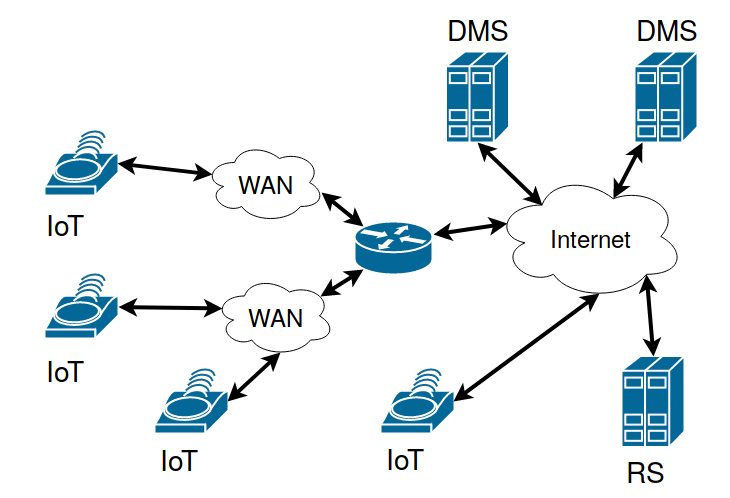
\includegraphics[width=200pt]{papers/ot/images/ot-fig-1.png}
\caption{An overview of the considered system}
\label{fig:system_0}
\end{figure}

In the scenario depicted in Figure \ref{fig:system_0}, the different IoT units are connected to the Internet and consequently vulnerable to all kinds of network based attacks. Hence, it is important that the IoT units are properly authenticated and that only well protected communications are allowed over the Internet and over the wireless network. In particular, independent of Internet access technology, there must be credentials in place on the IoT units so that they can securely perform mutual authentication with the back-end system. 
For an ownership transfer to take place we assume that there exists another organization, with its own DMS, to transfer the ownership to. 


We furthermore assume the existence of a trusted third party in the form of an RS. RS i operated by an organization that both organizations trust to a high degree. The RS will facilitate the ownership transfer process.
The RS and DMS are not constrained in what types of cryptographic operations they can do i.e. asymmetric cryptography is possible. We also assume that the DMS servers and RS can exchange keys and authenticate each other, possibly with a PKI. The cryptographic functions are assumed to be secure.

\section{Adversarial model and problem description}
\label{threat-model}
\subsection{Adversarial model}
\label{adversary}
Similar to many existing work in IoT and cloud security, we assume that the adversary is acting according to the Dolev-Yao adversarial model \cite{Dolev1981}. This means that an attacker is able to intercept, delete, change order or modify all messages sent over the communication channel between any entity. The adversary can also destroy messages, but is not able to break cryptographic functions. Furthermore, we assume the IoT nodes are placed into an environment such that physical attacks from an insider adversary (such as the current owner) have to be considered while the DMS and the RS are assumed to be in a secure location or in protected isolated environments protected from both external and insider software attacks.

With respect to the direct physical attacks on the IoT units, we assume that an adversary as well as the old and new DMS are able to compromise, with a given effort, some or a limited number of IoT units through direct physical attacks on the devices. Here a compromised node refer to a node where the attacker has full control of the execution environment as well as volatile and persistent storage units of the device. Such a model is motivated by the fact that the needed effort for direct physical attacks is at least proportional to the number of compromised units.  Attacks from the current or new owner on a large scale can be very hard to perform in practice due to hardware protection mechanisms on the IoT units for instance.
\subsection{Trust model}
 The RS is assumed to be ‘’honest but curious’’ \cite{Oded2009}, which means the RS will be a legitimate  participant in protocol interactions. It will not deviate from the defined protocol, but will attempt to learn all possible information from legitimately received messages. The Old Owner and the New Owner are assumed to not fully trust each other, i.e. the Old Owner has interest in learning the secrets used by the New Owner. Similar, the New Owner would like to get hold of the secrets used by the Old Owner.

\subsection{Requirements}
\label{requirements}
Given the previously introduced adversary model, we have looked over the general ownership transfer security requirements identified in previous work on RFID tags \cite{taqieddin2018tag} and adapted them to our system and adversary model: 
\begin{labeling}{R11.}
%\item [R1.] \textbf{Ownership transfer security:} The protocol shall net allow any outside entity to learn credentials for any party in the system.
\item [R1.] \textbf{IoT unit impersonation security:} The protocol shall not allow an adversary to impersonate legitimate IoT units during or after ownership transfer.
\item [R2.] \textbf{Old DMS impersonation security:} The protocol shall not allow an adversary or the new DMS to impersonate the old DMS.
\item [R3.] \textbf{New DMS impersonation security:} The protocol shall not allow an adversary or the old DMS to impersonate the new DMS.
\item [R4.] \textbf{RS impersonation security:} The protocol shall not allow an adversary, any IoT unit or any DMS in the system to impersonate the RS.
\item [R5.] \textbf{Reply attack resistance:} The protocol shall be resistant against attacks where an adversary tries to complete sessions with any entities in the system by replaying old, observed messages.
\item [R6.] \textbf{Resistance to Man-in-the-Middle attacks (MitM):} The protocol shall not allow insertion or modification of any messages sent between trusted entities in the system.
\item [R7.] \textbf{Resistance to de-synchronization attack:} The protocol should not allow the IoT units and the new or old DMS to enter a state where necessary secure communications is prevented by a credential mismatch. 
\item [R8.] \textbf{Backward security:} During and after an IoT ownership transfer, the new owner shall not be given access to any secrets allowing the new owner to get access to any identities or confidential information used in past sessions between the old DMS and the IoT units.
\item [R9.] \textbf{Forward security:} During and after an IoT ownership transfer, the old owner shall not be given access to any secrets allowing the old owner to get access to any identities or confidential information used in sessions between the new DMS and the IoT units.
 \item [R10.] \textbf{No double ownership:} There shall not be any time period during the ownership transfer process when both the old and the new owner has control over an IoT unit in the system.
\end{labeling}

In addition to these requirements, our adversary model does not imply full trust in the RS and we also take into account the risk of that IoT units might be compromised through direct physical attacks. These two assumptions give the following additional two requirements:

\begin{labeling}{R12.}
\item [R11.] \textbf{Protection of new credentials :} After the completion of the ownership transfer, the RS shall not have knowledge of the new IoT credentials and shall not be able to set impersonate the new DMS or have access to secure sessions between the new DMS and the IoT units in the system.
\item [R12.] \textbf{IoT compromise resilience:} A successful compromise of an IoT unit by an external or internal adversary shall only give the adversary the power to impersonate this single IoT unit in the system and not impersonate or break any secure sessions between other, non-compromised IoT units in the system and the new DMS.
\end{labeling}

In many IoT infrastructures, some IoT units are placed in local networks not publicly open but they are accessible by the owner system only. In our case, this means that the current DMS can access the units but not for instance an external entity like the RS. Opening up the system and allowing direct interactions between all IoT units in the system and the RS is a potential security risk. Hence, we have the following additional requirement on the system solution:

\begin{labeling}{R13.}
\item [R13.] \textbf{IoT unit isolation:} An ownership transfer shall not require any direct interactions between the IoT unit and the RS but only between the IoT unit and the DMS (old or new) in the system.
\end{labeling}
\subsection{Problem statement}
\label{problem}
We want to transfer the ownership of a set of deployed IoT devices from one entity to another. Each IoT device has some form of credentials that it shares with a remote entity. Ownership is defined as holding the credentials of the individual IoT-nodes. Ownership transfer then is the process of updating the credentials from keys shared with the old owner to keys shared with the new owner. We want to find an ownership transfer protocol and solution secure under the previously defined threat model and which meets the identified security requirements in Section \ref{requirements}.

\section{IoT infrastructure ownership transfer model and protocol design}
\label{Solution}
The ownership transfer process can, according to our solution, be divided into three phases:
\begin{itemize}
\item Deployment
\item Ownership transfer preparation
\item Ownership transfer
\end{itemize}
In the deployment stage the RS and the first owner provisions keys to the individual devices, the devices are then deployed.

In the ownership-transfer preparation phase, the owner, now called old owner, and the new owner signs a list of all devices that shall be transferred and forwards this list to the RS. The RS then distributes the needed keys for the transfer and generates an ownership transfer token as well as the individual keys to the new owner.

In the final ownership transfer stage, the old owner sends the ownership transfer token to the IoT units. After receiving the token the IoT devices verify and decrypt the token. The information in the token is used to contact the new owner. The new owner and the IoT units then authenticate each other and new credentials are provisioned to the IoT devices. The detailed protocol description is done in the subsection below, using terminology defined in Table \ref{tab:notation}, and illustrated in Figure \ref{fig:proto-2}. The steps from Figure \ref{fig:proto-2} are references by bold numbers e.g. \textbf{(1.1)}.

\begin{table}

\footnotesize{
\begin{tabularx}{.47\textwidth}{l m{5cm}}
%\begin{tabular}{ll}
%\begin{tabular}{*{5}{p{3cm}}}
\hline
      $DMS_{old}$ & Old Device Management Server  \\
      $DMS_{new}$ & New Device Management Server  \\
      $RS$ &Reset server  \\
    
      $Sign(P, d)$ & Digital signature of data $d$ by party $P$.  \\
      $E(k,m)$  & Symmetric encryption of message $m$ with key $k$.  \\
      $D(k,c)$  & Symmetric decryption of ciphertext $c$ with key $k$.  \\
      $MAC(k,m)$  & Message Authentication Code of message $m$ with key $k$.  \\
      $PRF(s)$ & Pseudo-random function with seed $s$, generating  \\
               & a pseudo random key. \\
    
      $IoT_i$  & IoT device number $i$.  \\ 
      $ID_i$  & Identifier of IoT device $i$. \\
      $ID_{new}$ & Identifier of $DMS_{new}$.  \\ 
      $URL_{new}$ & Uniform resource locator to $DMS_{new}$.  \\ 
      $K_i$ & Key for IoT device number $i$, shared with $RS$  \\ 
      $KR_E$ & Reset-key used for encryption.  \\ 
      $KR_M$ & Reset-key used for message authentication.  \\
      $KO_i$ & Owner-key for IoT device number $i$, divided into two parts $KO_i = \{KO_{i1}, KO_{i2}\}$  \\
      $K_{RS}$ & Master-key for $RS$ used for deriving $K_i$.  \\

      $N$ & Ownership-transfer nonce.  \\
      $Ctr_i$ & Counter for node $i$ is used for verifying freshness  of nonces.  \\
      $Ctr_{RS}$ & Counter for $RS$, incremented at every ownership transfer. Used for verifying freshness of nonces.\\
      $KS_i$ & Ownership transfer key for node $i$ composed by: $KS_i = PRF( K_i || N || Ctr_{RS})$ \\
       $T$ & Ownership-transfer token, calculated by:  \\
          & $T = E(KR_E, ID_{new} || URL_{new} || N || Ctr_{RS} ||$ \\
          &$ MAC(KR_M, ID_{new} || URL_{new} || N || Ctr_{RS} ))$  \\
      $PSK_i$ & DLTS-PSK for IoT device $i$, generated by $PSK_i = PRF(KS_i || KO_{i2})$ \\
      \textbf{ID} & List of IoT device identities \textbf{ID} $= \{ID_1, ID_2, ... , ID_i\}$ \\
      \textbf{ID-K} & List of pairs of  IoT device identities and $KO_{i2}$:  \\
                    &  \textbf{ID-K} $= \{(ID_1,KO_{12}),  ... , (ID_i, KO_{i2})\}$ \\
      \textbf{K} & List of keys $K_i$ \textbf{K} $= \{K_1, K_2, ... , K_i\}$ \\
      \textbf{KO} & List of owner-keys $KO_i$, \textbf{KO} $= \{KO_1, KO_2, ... , KO_i\}$ \\
      \textbf{KS} & List of keys $KS_i$, \textbf{KS} $= \{KS_1, KS_2, ... , KS_i\}$ \\
      \textbf{ID-KS} & List of IoT device identities and keys: \\
                     &  \textbf{ID-KS} $= \{(ID_1, KS_1), ... , (ID_i, KS_i)\}$ \\
          \hline
%\end{tabular}
\end{tabularx}
} %tiny
\caption{Notations used in protocol description.}
\label{tab:notation}
\end{table}

\subsection{Deployment}


$RS$ generates the keys $KR_E$, $KR_M$ and $K_{RS}$. $RS$ provides each IoT device with a unique identifier $ID_i$. $K_{RS}$ is then used to generate $K_i$ for each $IoT_i$ by calculating $K_i = PRF(K_{RS} || ID_i)$. Each device $IoT_i$ is provided with the corresponding $KR_E$, $KR_M$, $ID_i$ and $K_i$. After transferring the keys $RS$ can discard all keys $K_i$. $RS$ sets its counter $Ctr_{RS} = 0$ and all IoT devices counters $Ctr_i$ are also set to zero. These counters are used to verify the freshness of the ownership tokens later on.
The first owner, $DMS_{old}$, takes control of the system and provides the owner-key $KO_i = \{KO_{i1}, KO_{i2}\}$ to each device $IoT_i$. The system is then ready for deployment and regular use, with $KO_i$ used for securing the communication with $DMS_{old}$. 

\subsection{Ownership transfer preparation}
The ownership transfer process starts with a preparation phase with interactions between the $RS$, $DMS_{old}$ and $DMS_{new}$. $DMS_{old}$ creates a list of all IoT device identities $ID_i$ called \textbf{ID} and a list of identities and partial keys $\{ID_i, KO_{i2} \}$ called \textbf{ID-K} that shall switch owner \textbf{(1.1)}. The list of identities is signed $Sign(DMS_{old}, \mathbf{ID})$. Both lists are sent to $DMS_{new}$ \textbf{(1.2)}, $DMS_{new}$ first verifies the signature of the list, the list of identifiers are then signed by $DMS_{new}$. The result is $Sign(DMS_{new}, Sign(DMS_{old}, \mathbf{ID}))$, the list \textbf{ID-K} is kept by $DMS_{new}$ \textbf{(1.3)}. The list \textbf{ID} is sent to $RS$, to prove that ownership transfer shall take place and that both $DMS_{old}$ and $DMS_{new}$ are agreeing to the transfer \textbf{(1.4)}. $DMS_{new}$ also sends its identifier and URL to $RS$.
After verifying that the list \textbf{ID} is correctly signed by both $DMS_{old}$ and $DMS_{new}$ \textbf{(1.5)}, $RS$ can start the ownership transfer protocol. 

\subsection{Ownership transfer}
$RS$ start the ownership transfer process by re-generating the keys $K_i$. A nonce $N$ is generated, that together with $Ctr_{RS}$ is used to generate the individual ownership transfer keys $KS_i = PRF(K_i || N || Ctr_{RS})$ \textbf{(2.1)}. The list of ownership transfer keys \textbf{ID-KS} is sent to $DMS_{new}$ \textbf{(2.2)}. The $RS$ creates the ownership transfer token $T$, with information needed by the IoT devices, authorizing an ownership transfer and information for how to do it. $T = E(KR_E, ID_{new} || URL_{new} || N || Ctr_{RS} || \\ MAC(KR_M, ID_{new} || URL_{new} || N || Ctr_{RS} ))$
$RS$ sends the token $T$ to $DMS_{old}$ \textbf{(2.3)}.
$DMS_{old}$ forwards the Ownership Transfer Token $T$ to all IoT devices \textbf{(2.4)}. The devices decrypts $T$ with $KR_E$ and verifies the MAC with $KR_M$. If the MAC verification succeed, the freshness of the nonce is checked by verifying $Ctr_{RS} > Ctr_i$ (\textbf{2.5}). After these checks each IoT device $IoT_i$ can compute the ownership transfer key $KS_i = PRF(K_i || N || Ctr_{RS})$ (\textbf{2.6}). With $KS_i$ and $KO_{i2}$ the IoT devices can connect to $DMS_{New}$ using DTLS-PSK\cite{rfc7925}. The parameters used are PSK-ID = $ID_i$ and PSK = $PRF(KS_i || KO_{i2})$ (\textbf{2.7}). After a successful contact has been made with $DMS_{new}$ $IoT_i$ destroys $KO_{i1}$ (\textbf{2.8}). $DMS_{new}$ then generates a new key $KO'_i$ (\textbf{2.9}). The new key $KO'_i$ is sent to $IoT_i$, that also sets $Ctr_i$ to the received value $Ctr_{RS}$(\textbf{2.10}). After $DMS_{new}$ has provisioned new keys to all IoT devices the ownership transfer process is concluded. $DMS_{new}$ can securely communicate with all IoT devices using the new keys $KO'_i$.

\begin{figure*}[h]
\centering
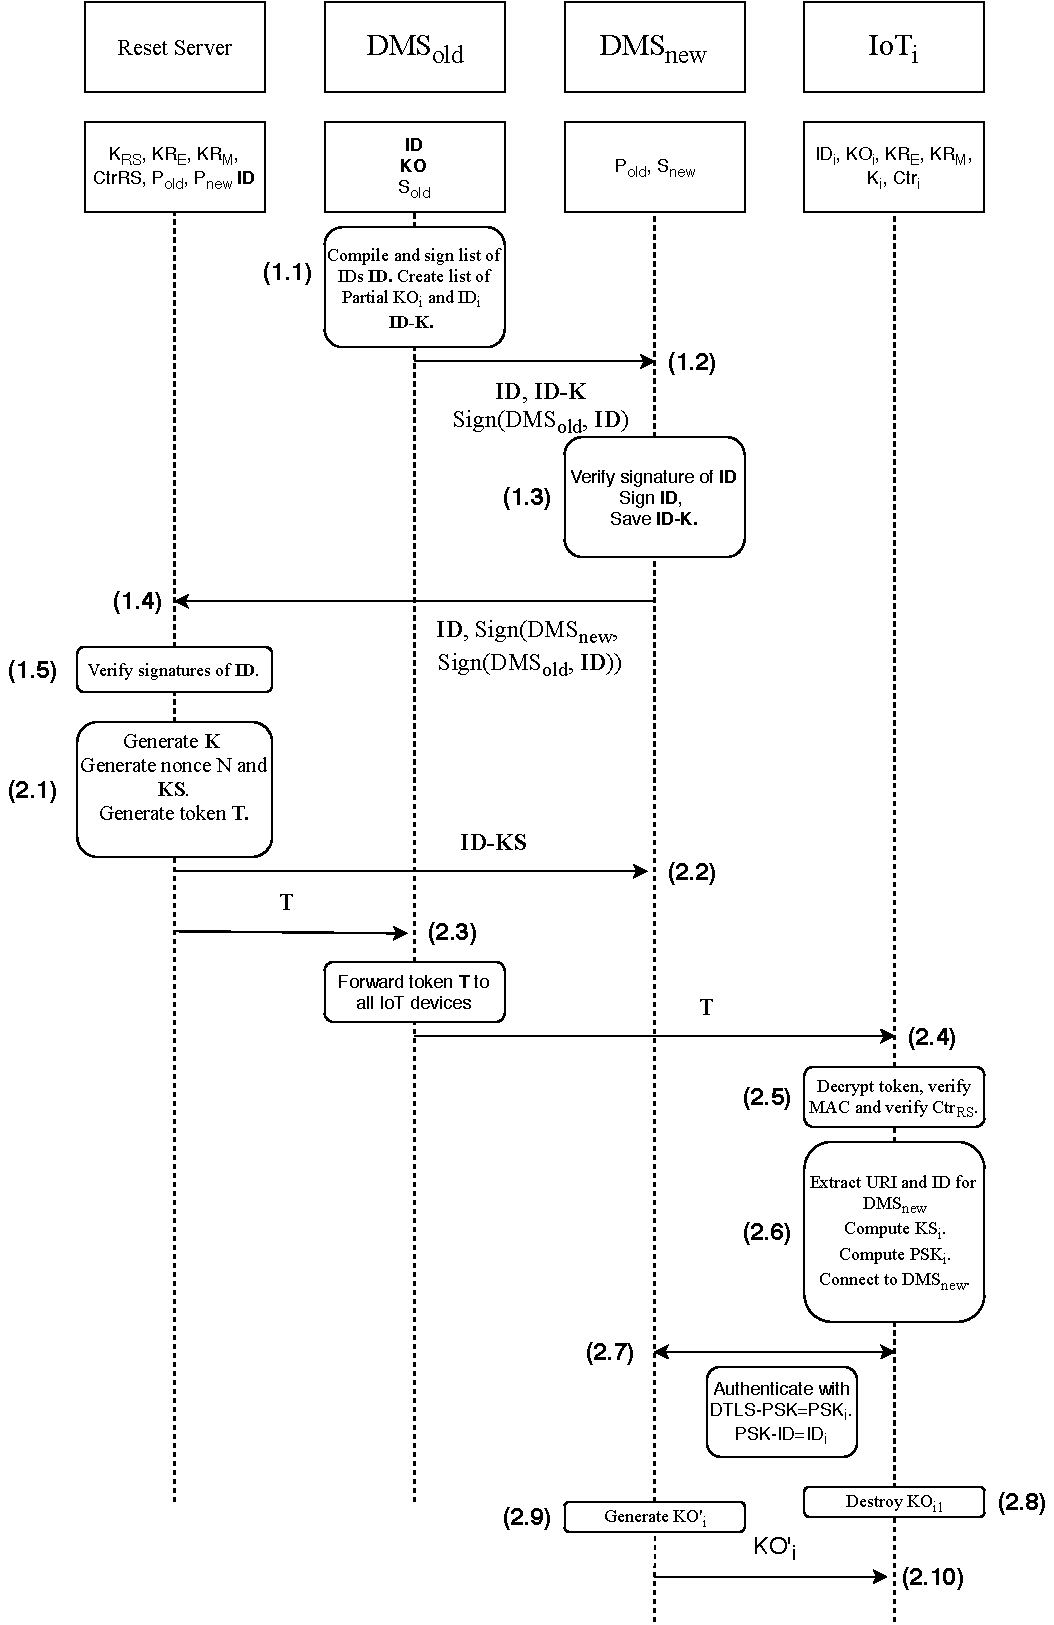
\includegraphics[scale=0.545]{papers/ot/images/ot-proto-2.pdf}
\caption{Messages and computations done during the ownership transfer.}
\label{fig:proto-2}
\end{figure*}

\subsection{Handling of ownership transfer failures}
\label{failures}
 In the previous sections we have described the ownership transfer process in detail. However, there is a risk that the ownership transfer succeeds for one set of IoT units but not for another set due to communication errors or similar. Such situation will be detected by the $DMS_{New}$ as it will notice that it has not been able get in contact and authenticate some units part of the IoT transfer list given in step 1.2. $DMS_{New}$ can first retransmit the ownership transfer token $T$ to the devices that has not changed ownership. Some protocols provide a mechanism of notifying a sender that a message has been received. Such a mechanism can be used to verify the proper delivery of $T$. If $T$ has been delivered but an IoT device still does not connect to $DMS_{New}$ the issue lies with the device $IoT_i$, that situation will have to be resolved by $DMS_{Old}$ before a new attempt can be made.  In such situation, it is possible is for $DMS_{New}$ to issue a ''recovery'' procedure by sending a signed list of missing units back to $DMS_{Old}$, which then will be requested to contact each of the missing IoT units (still under ownership of $DMS_{Old}$) over a mutual authenticated DTLS channel re-sending the transfer token, $T$. Such procedure can be repeated, until the whole set of IoT units are successfully transferred to $DMS_{New}$.

\section{Implementation and experimental evaluations}
\label{Implementation}
We have implemented our proposed protocol for an IoT environment running Contiki-NG\footnote{ \url{https://github.com/contiki-ng/contiki-ng}}. Contiki-NG is a light-weight operating system designed for constrained devices. We have used some other protocols to structure our data. Most significantly we use COSE \cite{rfc8152} to encode and encrypt the ownership transfer tokens. We assume secure communication between the $RS$, $DMS_{old}$ and $DMS_{new}$. The connections to the IoT devices are secured with DTLS\cite{rfc6347}. 

We have designed the system to use the REST-model\cite{fielding2000representational}. Sending the ownership transfer token to the IoT device is done with a PUT operation to /transfer-ownership. The IoT device then sends a GET message to /key to receive the new keys $K'_i$ and $KO'_i$. 


\subsection{Test Setup}
The evaluated scenario is executed on the following setup. One Desktop PC running the $RS$, $DMS_{Old}$ and $DMS_{New}$. The PC is connected to a Border-Router that acts as an IEEE 802.15.4 network interface. We have used four Zolertia Firefly-A development boards\footnote{\url{https://github.com/Zolertia/Resources/wiki/Firefly}} that are going to transfer from owner $Old$ to $New$. The IoT devices are based on the cc2538 system on chip made by Texas Instruments\cite{instruments2015cc2538}. They have an ARM Cortex-M3 CPU clocked at 32MHz together with 32KB of RAM and 512KB of flash. Connectivity is provided by an IEEE 802.15.4 radio providing about 100Kb/s of bandwidth. 

\subsection{Test Scenario}
The test scenario consists of an initial setup phase where keys are distributed to the individual IoT nodes and an ownership transfer phase. The initial setup phase is not in scope for the performance evaluation, only the ownership transfer process is included. We ran the ownership transfer scenario, of the four IoT devices, ten times.

\subsection{Ownership transfer time}
In order to evaluate the efficiency of our proposed scheme from a system perspective we timed the entire ownership transfer process. We measured the time elapsed from that the $RS$ sends out the token $T$ to when all IoT devices has been provisioned with new owner keys $KO'_{i}$.
The time taken for the ownership transfer process is measured to a mean of 4.7s with a 95\% confidence interval between 4.4s and 5s.

\subsection{Energy consumption}
Since the devices considered for this protocol usually are powered by a battery it is important that the energy consumed by the IoT device when executing the ownership transfer protocol is reasonable.

We have measured the energy usage on the constrained nodes for both the radio modem and the CPU. The total energy consumption was measured to a mean of 0.18mJ. With a 95\% confidence interval of the mean between 0.14mJ and 0.22mJ. For comparisons sake, the mean energy consumption of 0.18mJ is equal to the energy consumed by the CPU executing at full power for four seconds.

\section{Security analysis}
\label{analysis}
We will now analyze our proposed ownership transfer protocol in the scope of the system model presented in Section \ref{System} and the threat model from Section \ref{threat-model}. We will address each requirement from \ref{requirements} except R13 that is a functional requirement. We give special attention to the requirements R8, R9 and the requirement for $PSK_i$ to be secure. We formally prove these requirements with Tamarin Prover\cite{basin2017symbolically}. The requirement to protect $PSK_i$ from an outside adversary is important for requirements R1, R3 and R6 while backward (R8) and forward (R9) secrecy are a core features of the suggested protocol.


%We will divide our analysis into two parts. The first part where we look at a system compromise from an involved party and a second part where we will analyze the security from outside adversaries. This analysis is aimed at the ownership transfer protocol and other scenarios are out of scope of this paper. 

\begin{labeling}{R12.}
\item [R1.] \textbf{IoT unit impersonation security:} Each IoT unit $i$ holds a unique key $K_i$. The nonce and counter in the token together with this key are used to calculate $KS_i$. In turn, $KS_i$ and the second part of $KO_i$ are used to calculate the PSK, used to authenticate the connection between the IoT unit and $DMS_{New}$. Both key parts needed to calculate the PSK are only known to $DMS_{New}$ apart from the IoT unit as long as the RS and old owner do not collude, which contradicts the trust assumption regarding the reset server. Hence, given that the IoT unit itself can securely store and keep $K_i$, IoT impersonation is not possible for an external attacker or $DMS_{Old}$. 
\item [R2.] \textbf{Old DMS impersonation security:} The ownership transfer is triggered by letting $DMS_{Old}$ send a signed list of IoT identities (step 1.2). This signature is verified by the RS at step 1.5. As long as the signature scheme is secure and the private key of the $DMS_{Old}$ not is compromised, an attacker cannot impersonate the $DMS_{Old}$ at the ownership transfer ''triggering moment''. As we do not require protected transfer of the token (step 2.4), $DMS_{Old}$ impersonation at this step is possible. However, it is not crucial for the protocol that it is indeed $DMS_{Old}$ that sends the token but it can be transferred in arbitrary way, as the IoT unit does not finally accept the token unless the authentication in step 2.7 is performed successfully. The latter requires the genuine key $KO_{i2}$ from old owner, and this key is sent protected to the $DMS_{New}$ at step 1.2. 
%The protocol shall not allow an adversary or the new DMS to impersonate the old DMS.
\item [R3.] \textbf{New DMS impersonation security:} %The protocol shall not allow an adversary or the old DMS to impersonate the new DMS. 
Similar to the  $DMS_{Old}$, $DMS_{New}$ signs the list of IoT IDs subject to ownership transfer (step 1.3). This signature is verified by the RS  at step 1.5. As long as the signature scheme is secure and the private key of the $DMS_{New}$ not is compromised, an attacker cannot impersonate the $DMS_{New}$ at the ownership transfer ''trigering moment''. Mutual authentication applies at step 2.7 when the IoT unit connects to the $DMS_{New}$. Impersonation at this step requires knowledge of the PSK, which (similar to the reasoning regarding R1 above), requires knowledge of both $KS_i$ and $KO_i$, and if not the RS and old owner collude, these two values are only known to $DMS_{New}$ and the IoT unit itself. Hence, $DMS_{New}$ impersonation is not possible unless $DMS_{New}$ is compromised such that the secure keys leaks or the secure key transfers at step 1.2 or step 2.2 are broken. The latter is not possible if not the mutually authenticated secure channel is weak.
\item [R4.] \textbf{RS impersonation security:} %The protocol shall not allow an adversary, any IoT unit or any DMS in the system to impersonate the RS.
Only $DMS_{New}$ and $DMS_{Old}$ communicate directly with $RS$. They do so over a secure channel that protects against impersonation of $RS$.
\item [R5.] \textbf{Reply attack resistance:} %The protocol shall be resistant against attacks where an adversary tries to complete sessions with any entities in the system by replying old, observed messages.
All messages between $RS$, $DMS_{Old}$ and $DMS_{New}$ are sent over secure channels that provides protection against replay attacks (steps 1.2, 1.4, 2.2 and 2.3). The Token $T$ transferred from $DMS_{Old}$ to $IoT_i$ (step 2.4) contains $Ctr_{RS}$ that is verified against $Ctr_{i}$ by $IoT_i$. This provides replay attack resistance since a replayed $T$ will be rejected due to the counter check. When $IoT_i$ connects to $DMS_{New}$ (step 2.7) it is done with DTLS protected by $PSK_i$, which is only known to $DMS_{New}$ and $IoT_i$. This DTLS channel is also used to protect the transfer of the new credentials $KO'_i$ (step 2.10).
\item [R6.] \textbf{Resistance to Man-in-the-Middle attacks (MitM):} %The protocol shall not allow insertion or modification of any messages sent between trusted entities in the system.
All messages between $RS$, $DMS_{Old}$ and $DMS_{New}$ are sent over secure channels that provides mutual authentication (steps 1.2, 1.4, 2.2 and 2.3) and thus prevents against MitM attacks. Communication with the IoT devices and $DMS_{New}$ (steps 2.7 and 2.10) is done over DLTS-PSK that provides mutual authentication and with MitM protection. An attacker with knowledge of the keys $KR_E$ and $KR_M$\footnote{These keys are included not to give protection against IoT compromise but to make denial-of-service type of attacks less likely.}, can perform a successful man-in-the-middle substitution attack at step 2.4. Potential values to substitute are $ID_{new}$, $URL_{new}$, $N$ or $Ctr_{RS}$. The IoT unit will not accept a wrong $Ctr_{RS}$ as it is checked against the internal counter. Furthermore, substituted $ID_{new}$ or $N$ will not match the PSK values used in the mutual authentication in step 2.7 and the MitM substitution attack will fail. A substitution of $URL_{new}$ will have no affect as long as the IoT unit still reach the legitimate $DM_{new}$ with the given URL. If this not is the case,the ownership transfer for the affected unit will simple be aborted (see also the recovery discussion in Section \ref{failures}).
%When $IoT_i$ connects to $DMS_{New}$ (step 2.7) it is done with DTLS using the key $PSK_i$ known only to $DMS_{New}$ and $IoT_i$ to outsider can launch a MitM attack since DTLS provides MitM mutual authentication. The same DTLS session is used when $DMS_{New}$ transfers the new credentials $KO'_i$ to $IoT_i$ (step 2.10).

\item [R7.] \textbf{Resistance to de-synchronization attack:} %The protocol should not allow the IoT units and the new or old DMS to end-up with different new credentials preventing them from communicating securely in the future.
If $DMS_{Old}$ should send a modified token, $T'$ (through access to the keys $KR_E$ and $KR_M$), with modified nonce $N'$, in step 2.4, the key $KS'_i$ will not match the key $KS_i$ held by $DMS_{New}$. Hence, in this case, the IoT device will not remove the $KO_i$ key, and will remain in the ownership of $DMS_{Old}$.
\item [R8.] \textbf{Backward security:} %During and after an IoT ownership transfer, the new owner shall not be given access to any secrets allowing the new owner to get access to any identities or confidential information used in past sessions between the old DMS and the IoT units.
All traffic sent between the $DMS_{Old}$ and the IoT devices is sent over a channel protected by the key $KO_i$, the IoT devices destroy $KS_i$ when contact is made with $DMS_{New}$. $DMS_{New}$ can not recover $KO_i$ and is unable to learn any previous secrets (see also the Tamarin proof of Section \ref{Tamarin}).
\item [R9.] \textbf{Forward security:} %During and after an IoT ownership transfer, the old owner shall not be given access to any secrets allowing the old owner to get access to any identities or confidential information used in sessions between the new DMS and the IoT units.
After $DMS_{New}$ has made contact with the IoT devices and the old key $KO_i$ has been destroyed, $DMS_{New}$ provisions a new key $KO'_i$ and sends it to the IoT devices over a secure channel protected by the key $KS_i$ that $DMS_{Old}$ does not hold. $DMS_{Old}$ is thus unable to decrypt any future message sent to the IoT devices  (see also the Tamarin proof of Section \ref{Tamarin}).
 \item [R10.] \textbf{No double ownership:} %There shall not be any time period during the ownership transfer process when both the old and the new owner has control over an IoT unit in the system.
 The ownership hand-over is made when the IoT device connects to $DMS_{New}$ with $PSK_i$ and removes ownership from $DMS_{Old}$ by removing $KO_i$. $DMS_{New}$ takes ownership when it provisions $KS'_i$ to $IoT_i$. Failure in any protocol step might results in that some IoT units are still owned by the $DM_{old}$. However, as we discuss in Section \ref{failures} below, such situation can be detected by $DMS_{New}$ and a recovery process can be initiated.
\item [R11.] \textbf{Protection of new credentials:} 
After the ownership transfer process $IoT_i$ is provided with new credentials $KO'_i$. The only way $RS$ can gain access to the system is by launching a MitM attack on the DLTS connection between $IoT_i$ and $DMS_{New}$. Thus this property hinges on $PSK_i$, $RS$ does not know $KO_{i2}$ needed to derive $PSK_i$. As long as $RS$ does not gain access to $KO_{i2}$ by collusion with $DMS_{Old}$, the new credentials are protected.
\item [R12.] \textbf{IoT compromise resilience:} 
If an adversary compromises an IoT device $IoT_i$ it will gain the following keys: $KO_i$, $KR_E$, $KR_M$ and $K_i$. $KO_i$ is only shared with the current owner and used for securing communication between the owner and IoT device, the adversary can not impersonate or compromise any other IoT device. $KR_E$ and $KR_M$ are shared with all IoT devices, an adversary could try to spoof an ownership transfer token $T$. Since the adversary only have $KO_i$ it is impossible for the adversary to complete a malicious ownership transfer with an other IoT device $IoT_j$ since the adversary does not know $KO_j$, thus providing resilience against compromises.
\end{labeling}

\subsection{Tamarin Prover}
\label{Tamarin}
Tamarin Prover is a tool for formal analysis of security protocols. By creating a symbolic model of a protocol, stating security lemmas and then using the automatic reasoning to analyse the model the prover can  show that the security lemmas hold or show a counter-example of when they do not hold.
Tamarin represents protocols as a multi-set rewrite rules using first order logic. The automatic prover represent the state of the execution as a bag of multi-set of Facts. The adversary model used in Tamarin is the Dolev-Yao model. %\cite{dolev1983security}. In the Dolev-Yao model the adversary is able to read, modify, replay and send any message to any participant in the system. One way of phrasing this, is to say that the adversary \textit{is} the network itself. 

\subsection{Modeling the Ownership Transfer Protocol}
We have modeled a simplified version of our proposed Ownership Transfer Protocol in Tamarin. We have excluded the steps 1.1 - 1.5 and 2.7 - 2.10 to prove the correctness of the core ownership transfer steps. During our process to verify the security of our proposed protocol we have introduced four lemmas.
We have created one lemma, Protocol Correctness, to verify that our protocol can execute with a successful conclusion of the ownership transfer process. We have created another lemma, Outsider secrecy, to prove that $PSK_i$ is secret from an outside adversary. The next two lemmas Old Owner Secrecy and New Owner Secrecy are lemmas about attacks done by a party in the protocol that misbehaves. These types of attacks are not included in a standard Dolev-Yao model. To solve this problem, we have chosen to give the Dolev-Yao adversary all keys and secrets from the malicious party. The Dolev-Yao adversary then has all the capabilities to intercept, replay and send any message together with the capability to decrypt, encrypt and sign messages with the keys from the malicious party. We argue that this is a stronger attacker than a real-world malicious Old owner or New owner would be.
We have assumed that to provide New Owner secrecy $PSK_i$ has to be kept secret from $DMS_{Old}$. To Provide Old Owner Secrecy the two keys $KO_{i1}$ and $KO_{i2}$ have to remain secret from $DMS_{New}$. For the Outsider Secrecy Property we state that no outside party can learn $PSK_i$. Our Tamarin model of our proposed protocol can be found here \footnote{\url{https://github.com/Gunzter/iot-ownership-transfer-protocol-tamarin-model}}.

Below we list the four lemmas:
\begin{labeling}{L4.}
\item[L1] \textbf{Protocol Correctness.} The modeled protocol shall execute as specified.

$lemma \, protocol\_correctness: \\
	exists\_trace \\
	" \exists \: PSK1 \: PSK2 \: \#i \: \#j. \\
	(( \, New\_owner\_PSK( \, PSK1 \, ) \, @ \: \#i \, ) \, \wedge \\
 	( \, IoT\_PSK( \, PSK2 \, ) \, @ \: \#j \, )) \, \wedge \\
	(PSK1 \, = \, PSK2)"$

 \item[L2] \textbf{Outsider secrecy.} The Ownership Transfer protocol shall be secure against outside attackers. No outside party shall be able to learn $PSK_i$.
$lemma outsider\_secrecy: \\
 	all-traces \\
	" \forall \: PSK \:  \#i \: \#j. \\
	(((( \, IoT\_PSK( \, PSK \, ) \, @ \: \#i \, ) \, \wedge \\
	   ( \, New\_owner\_PSK( \, PSK \, ) \,  @ \: \#j \, )) \, \wedge \\
	(\neg(\exists \, Old\_owner \: \#k. \, Reveal( \, Old\_owner \, ) \,  @ \: \#k))) \, \wedge \\
	(\neg(\exists \, New\_owner \: \#l. Reveal( \, New\_owner \, ) \,  @ \: \#l)))  \,  \rightarrow 
	( \neg (\exists \: \#k. \, K(PSK) \,  @ \: \#k))" $
 
 \item[L3] \textbf{Old Owner secrecy.} The New Owner shall not be able to learn anything that has been sent before the ownership transfer, thus $KO_{i1}$ and $KO_{i2}$ has to be secure against an adversary that knows everything $DMS_{New}$ knows. 
  $lemma backwards\_secrecy: \\
	all-traces \\
	" \forall \: New\_owner \: PSK \: \#i \: \#j \:  \#k. \\
	((((\,IoT\_PSK(\, PSK \,)\, @ \: \#i \,) \, \wedge \\
	   (\, New\_owner\_PSK(\, PSK \,)\, @ \:  \#j\,))\, \wedge \\
	   (\, Reveal(\, New\_owner\, )\, @ \: \#k))\, \wedge \\ 
	    ( \neg ( \, \exists \,  Old\_owner \: \#l. \, Reveal( \,  Old\_owner \,  ) \,  @ \: \#l))) \, \rightarrow \\
	( \neg (\exists \: OwnerKey1  \: OwnerKey2 \: \#m \: \#n. \\
	( K(OwnerKey1) @ \: \#m) \wedge (K(OwnerKey2) @ \: \#n) ))" $
	
 \item[L4] \textbf{New Owner secrecy.} The Old owner shall not be able to learn anything that occurs after the ownership transfer is complete. No adversary that knows everything $DMS_{Old}$ shall be able to learn $PSK_{i}$. 

	$lemma forward\_secrecy: \\
	all-traces \\
	" \forall \: Old\_owner \: PSK \: \#i \: \#j \:  \#k. \\
	((((\,IoT\_PSK(\, PSK \,)\, @ \: \#i \,) \, \wedge \\
	   (\, New\_owner\_PSK(\, PSK \,)\, @ \:  \#j\,))\, \wedge \\
	   (\, Reveal(\, Old\_owner\, )\, @ \: \#k))\, \wedge \\ 
	    ( \neg ( \, \exists \,  New\_owner \: \#l. \, Reveal( \,  New\_owner \,  ) \\  @ \: \#l))) \, \rightarrow 
	( \neg (\exists \: \#m. K(PSK) @ \: \#m ))" $
	
	
\end{labeling}


Using our modeled protocol we let Tamarin prove the four stated lemmas. All of them were found to hold. We conclude that our protocol gives us the required security properties. 


\section{Conclusion}
\label{Conclusion}
In this paper we have identified the need for a light-weight, i.e. symmetric key based, ownership transfer protocol for IoT devices. We have studied the related field of ownership transfer for RFID tags and, inspired by previous work, identified the main security requirements for IoT infrastructure ownership transfer. A novel protocol was then constructed. We believe the proposed scheme fulfils all the identified requirements. The protocol was verified in a proof-of-concept implementation and shown to be indeed as light-weight as expected. The transfer-time is non-negligible for resource constrained IoT units, but on the other hand, ownership transfer typically happens quite rarely.  We performed a security analysis of the proposed scheme with special attention to the backward and forward secrecy with respect to old and new owner. These security properties were formally proven using the Tamarin Prover. 

Since the field of ownership transfer protocols and mechanisms in IoT is relatively unexplored we see many approaches for further work. Evaluating the performance of protocols in very large infrastructures, i.e. in the order of ten to hundred thousand IoT units. We would also like to verify the protocol in real systems such as industrial control systems or building automation. Investigating other approaches to the solution where no trusted third party is involved is also an interesting avenue of research. Lastly, since the field of IoT is in its infancy it would be interesting to look into more complex ownership models with multiple owners and the ability to temporary transfer ownership and control, i.e. to lend or rent, the IoT devices to another entity for a limited time.

{\raggedright
        \printbibliography[segment=\therefsegment,heading=subbibliography]
}
}





\fi

\ifpaperII
\newrefsegment
\addtolength{\apa}{2cm}
\fancyhead[RE]{\truncate{.95\headwidth}{\paperref{ch:ppiot}: \paperIItitle}}
\chapter[\paperIItitle]{\texorpdfstring{%
                \paperIItitle}{%
                \paperIItitle}}


\paperRemark{This is the full version of the paper below.
        This version contains an extended background description, and a more detailed motivation behind choices in the implementation as well as evaluation.

        \paperIIref}

{


\section{Introduction}
\label{introduction}
Internet-of-thing (IoT) is a network of physical objects or \emph{things} embedded with electronics, software, and sensors, connected through the Internet to collect and exchange data with manufacturers, operators and other connected devices. IoT includes a variety of connected objects from tiny stuff (e.g. smart dust) to enormous stuff (e.g. an entire city). Most IoT devices are used in factories, businesses and healthcare systems. By 2025, there might be more than 75.4 billion connected devices \footnote{https://www.statista.com/statistics/471264/iot-number-of-connected-devices-worldwide/} 
generating 175 trillion gigabytes of data\footnote{https://www.seagate.com/gb/en/our-story/data-age-2025/}, 
and total global worth of IoT technology would reach to USD 6.2 trillion by 2025\footnote{https://www.intel.com/content/www/us/en/internet-of-things/infographics/guide-to-iot.html}. 
This trend opens up to completely new possibilities with respect to data analysis services utilizing device data from a huge number of distributed devices \cite{Marjani2017}. The applications are very wide-ranging from healthcare and market analytics to industrial systems. In this paper, we consider big data IoT analytics from a privacy perspective. Even if the IoT units producing the data are not necessarily owned by an individual, the data they produce as well as communication patterns can reveal important business and industry secrets which should be avoided whenever possible \cite{Sadeghi2015} \cite{Maple2017}.

Huge scale analytic on powerful, third-party back-end cloud resources raises security and privacy concerns. One problem is that typically the cloud computing resources cannot be fully trusted. Another related problem is that if an adversary is able to observe the analytic operations or data storage read/write requests, sensitive information might be leaked. One way to tackle this problem is to use privacy-preserving cryptographic techniques \cite{Papadimitriou2016} \cite{Popa2011}, \cite{Wang2017}. However, so far these approaches have large overhead and thus severely limits the type of analytic operations that can be supported in the system. Especially the area of fully homomorphic encryption has achieved lots of attentions even if it is not yet fully practical \cite{Acar2018}.  An alternative approach is to operate on original data using analytic engines executed in Trusted Execution Environments (TEEs) such as Intel\textquotesingle s SGX. This line of research has gained quite a lot of attention during the past years \cite{Xu2018}\cite{Zheng2017}\cite{Schuster2015}. In these approaches, it is assumed that the data subject to data analysis is \emph{already} encrypted with a suitable encryption key available to the trusted application running in the TEE. Hence, before these protection techniques can be applied, the database content must be properly encrypted with the expected keys. In a scenario, where a large amount of IoT devices regularly uploads new data items subject to analysis, the data items must also be protected prior to arriving at the cloud storage resources \emph{and} they should be protected \emph{end-to-end}  without leaking any information about the source IoT unit. How to perform such encryption in an identity privacy-preserving and efficient way is the problem tackled in this paper. 

One key difference that needs to be taken into account when designing an IoT system solution is that in many applications, the IoT devices are resource-constrained \cite{Mun2016}.  They can, for instance, be constrained both in terms of computation power, as well as, being energy-constrained since they can be powered by a battery. Besides being more resource-constrained, they are also often deployed in a decentralized manner. These constraints limits, to a varying degree, what kind of security mechanisms that can be put in place, as well as, what kind of algorithms that can be executed on the IoT units \cite{Roman2011}. Hence by efficient, we here mean to avoid the trivial solution using public key encryption, which both is costly on the resource-constrained devices as well as when processing a large number of data items on the cloud resources.

Using a model of the availability of trusted computing engines in the cloud like the solutions in \cite{Zheng2017} and \cite{Schuster2015}, we consider the \textit {additional} and \textit{orthogonal} security problem of privacy preserving data cloud upload of IoT subject to data analysis. Especially, we consider this problem in the context of {\textit not} requiring any public key operation on the data collection, i.e. IoT, side but pure symmetric operations. Furthermore, we require IoT  \textit{individual} symmetric encryption keys as global encryption keys constitute a major security risk (a compromise of a single IoT unit will destroy the security for all or many devices).  In this context, the main challenge is to design a symmetric data encryption scheme allowing fast encryption and decryption while preventing an attacker, observing the data in transfer or at cloud storage, deducing any information bout the data origin like the identity of the IoT unit producing the data. Still, it must be possible for the analytic engines running at the cloud resources to efficiently to decrypt the data. We address this challenge suggesting an data item identity preserving encryption scheme and corresponding key management scheme.

The main contributions of the paper are the following:
\begin{itemize}
    \item We identify main security requirements for large scale, light-weight and identity privacy preserving, individual IoT data encryption and give formal security definitions.
    \item We present a novel encryption and corresponding key management scheme meeting the identified requirements.
    \item We evaluate the security properties of the proposed scheme and prove the security of the scheme for a couple of different attacker scenarios.
    \item We present a proof of concept implementation of the encryption scheme and make a performance evaluation.
\end{itemize}

We proceed as follows: we present the system scenario we are considering (\S \ref{Systemscenario}), we introduce our adversary model and derive security requirements as well as make formal security definitions (\S \ref{requirements}),  we give an overview of our novel IoT data encryption scheme and introduce notations (\S \ref{design}), we describe our proposed key management solution (\S \ref{keymanagement}), we present the detailed data encryption and decryption procedures (\S \ref{dataprotection}),  We make a formal security analysis of the proposed solution (\S \ref{secanalysis}) and present a proof of concept implementation, including performance figures (\S \ref{peranalysis}). Lastly we discuss related work (\S \ref{relatedwork}) and conclude (\S \ref{conclusion}).


\section{System scenario}
\label{Systemscenario}
We consider a system consisting of distributed IoT units, a management domain and a third-party cloud back-end (cloud provider) responsible for IoT data storage as well as data analytic operations.  Figure \ref{fig:systemarchitecture} depicts an overall system scenario which includes the following components: 

\begin{figure*}[th]
    \centering
    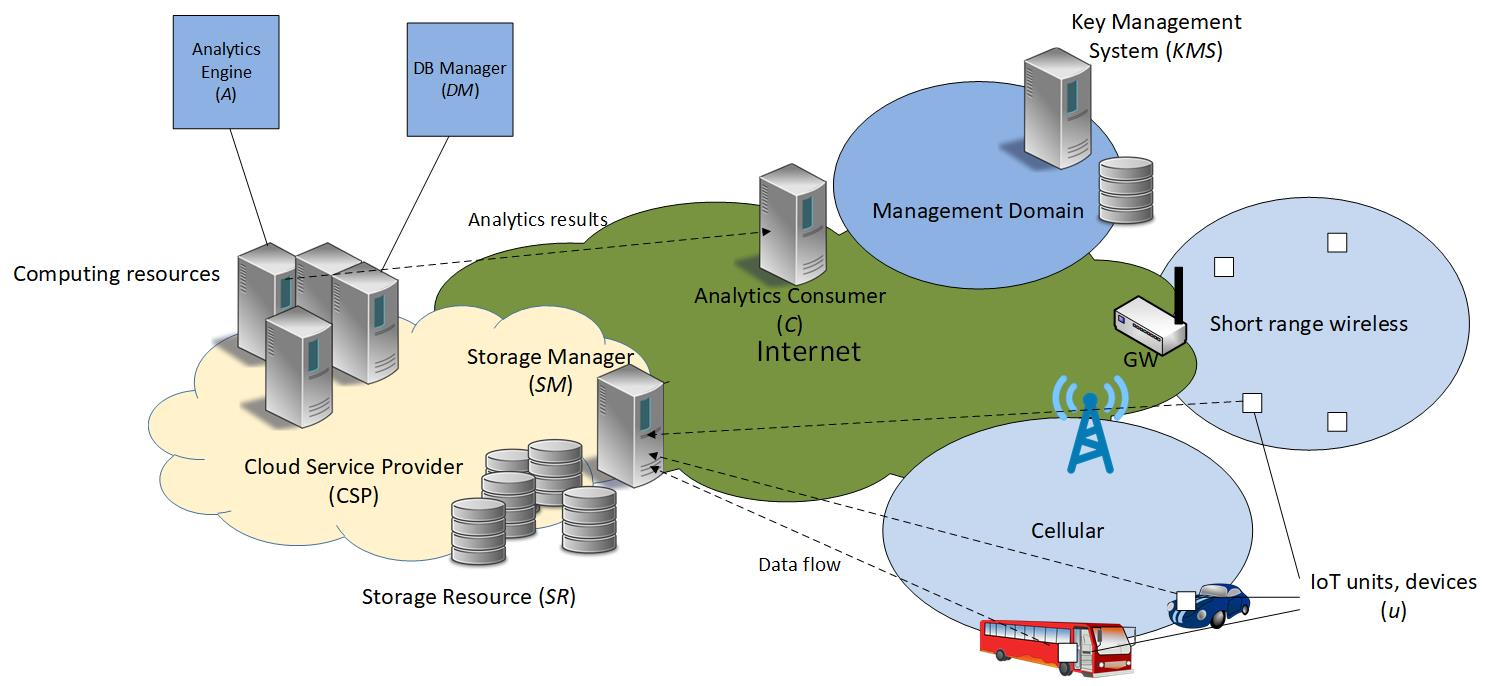
\includegraphics[width=400pt]{papers/ppiot/images/SystemArch}
    \caption{System scenario.}
    \label{fig:systemarchitecture}
\end{figure*}

%The different introduced components in the scenario and their notations are as follows:
\begin{itemize}
\item The Key Management System ($KMS$) deployed in a management domain is responsible for generating different credentials for IoT units and cloud execution containers, as well as the other entities running at a Cloud Service Provider (CSP) that need key material. The $KMS$ may also collect analytic results. 
\item CSP Storage Resource ($SR$), which is a repository responsible
for storing IoT data. 
\item Storage Manager ($SM$) which is the interface for collecting and accepting IoT data and storing it on the SR.
\item IoT units or what we refer to as devices ($u$) producing data which is sent securely to the SM component. The architecture is agnostic with respect to how the devices are deployed and in what type of network. All devices are assumed to have global network connectivity.
\item Database Manager ($DM$) responsible for sharing IoT data with analytic engines. The DM is deployed in a suitable execution container on the cloud resources in the form of a Virtual Machine (VM) or in a protected execution container like SGX.
\item Analytical engines ($A$) perform data analytics on IoT data through the DM. The analytics engines in the system are deployed on suitable execution containers on the cloud resources in the form of  Virtual Machines (VMs) or in protected execution containers like SGX.
\item Aanalytics consumer ($C$) which is authorized to receive analytics results produced by an A.
\end{itemize}

The boundary of the CSP is the space that contains $SM, SR, DM$ and $A$. The management domain might also be deployed in an cloud environment but must in the model we are considering be fully trusted. We discuss the adversary model and requirements in the next section. 

\section{Problem setting}
\label{requirements}
Next, we discuss the details of the data protection problem we are considering. We start by defining our adversary model and use this model to identify privacy requirements. Although the system scenario and architecture we are considering implies several additional requirements, the focus here are on the privacy/security requirements under the assumption of resource constrained IoT units. Next, we identify security and functional requirements on the system we are considering. Finally, we give formal security definitions. 
\subsection{Adversary model}
\label{requirements:adversary}
We consider a powerful adversary who may control the CSP network domain as well as having access to the $SM$ and $SR$. We do not consider denial-of-service (DoS) types attacks on these nodes though and assume that $SM$ and $SR$ are being able to operate properly. The adversary might also try to get full access to the computing resources but we assume the $A$ and  $DM$ to be deployed in secure containers using secure launch in combination with secure VMs or secure launch of SGX machines. Hence, the adversary has no possibility to directly modify or eavesdrop $A$ or $DM$. This model is motivated, as we stated in the introduction, with reference to trusted computing techniques in combination with secure launch as reported in \cite{Paladi2017} and protected SGX analytics as described in \cite{Schuster2015}. Recent attacks like Metldown \cite{Lipp2018} and Spectre \cite{Kocher2019}  have shown that one cannot even trust the fundamental hardware functions needed for secure isolation currently in use. Despite this fact, the security with respect to secure execution environment for virtualized systems is steadily improving and we will in this paper disregard attacks on the isolation properties of the execution containers. 

In line with many other works on IoT and cloud security, we assume that the adversary is acting according to the Dolev-Yao adversarial model \cite{ Dolev1981}. This implies that an attacker is able to intercept, delete, change order or modify all communication messages sent over the communication links between the IoT units and the CSP domain. The adversary can also destroy messages but is not able to break any cryptographic mechanisms. The devices are assume to be semi-trusted. This means that as long as an external attacker has not compromised a unit, it will be trustworthy. However, we do not exclude the possibility of that a limited set of the IoT units in the system are completely taken over by the adversary. 

The management domain including the $KMS$ is assumed to secure not in the control of the adversary.

\subsection{Requirements}
\label{requirements:requirements}
Starting from the previously presented system architecture and the given adversarial model, we have identified the following security requirements:
\begin{labeling}{R4.}
\item [R1.] \textbf{Data items confidentiality:} All data items sent from a device $u$ needs to be confidentiality protected, all the time, until they are processed by $A$ in a secure execution environment.
\item[R2.] \textbf{Data items integrity:} All data items sent from a device $u$ needs to be integrity protected, all the time, until they are processed by $A$ in a secure execution environment.
\item[R3.] \textbf{Analytics results confidentiality and integrity:} All analytics results must be confidentiality and integrity protected before they are returned to the $C$. 
\item[R4.] \textbf{Data items identity privacy:} It shall not be possible for an external adversary or a compromised IoT unit, $u'$ to determine which data item that is produced by a, non compromised, specific IoT unit, $u$. This implies that it shall not be possible to trace data items from different IoT units through potential identities used in protected data items.
\end{labeling}
Many of the devices might be placed in internal network not accessible from the outside. Furthermore, a particular device, $u$, might for security reasons be restricted not to set up secure sessions with external entities. It might also be an advantage if several data items can be buffered at an intermediate node, before they are transferred to the $SM$ for storage. Altogether, this gives us the following additional design requirement on the wanted solution:

\begin{labeling}{R5.}
\item [R5.] \textbf{IoT unit isolation:} A data transfer from $u$ shall not require any direct interactions (session) between the IoT unit and the $SM$.
\end{labeling}
Among these, requirements, it is particular challenging to fulfill requirement R4 in combination with R1 and R2 for the scenario we are considering. This is due to the fact, that it shall be possible for analytic engines deployed in the cloud, to quickly decrypt data items uploaded to the cloud using symmetric encryption only. This on the other hand, requires that the symmetric key for the data items must be available which in turn typically means that the data item must be ''marked'' with a key identity to allow symmetric key lookup. If a fixed identity is used, we do not fulfil R4 and this is the main security design challenge we address in this paper.

\subsection{Formal security definitions}
\label{requirements:secdefinitions}
Next, we give formal security definitions. We here focus on formally defining R1, R2 and R4. The reason for this choice  is that R3 can be fulfilled with standard secure channel and security association techniques and it is not the main problem we address here even this is a requirement for  a complete system solution. Furthermore, R5 is not a security requirement as such, but a property on the solution we want to have in order to offer practical and broadly applicable solution. Hence, we here do not either give a formal definition for R5.

Denote by $u\in U$ an arbitrary IoT unit and by $m \in M_n$, where $M_n$ is a plain text space index by $n$ (message of length $n$ bits), a data item produced by such unit. Furthermore, let $K_e \in {\cal{K}}_e$  and $K_{mac} \in {\cal{K}}_{mac}$, be a symmetric encryption and integrity keys respectively, known to the $u$ and the $DM$. We then denote by $c = E_{K_e}(r,m)$ the encryption of $m$ with Initialization Vector (IV) $= r \in R$ and using a suitable symmetric encryption algorithm, $E$. Similar, we denote by $x = \text{MAC}_{K_{mac}}(m)$, the message tag calculation for a message, $m$, using a suitable MAC function , MAC\footnote{In the scheme we consider the encryption and message authentication message scopes are not always the same. However, for simplicity, we here just use the notion of $m$ for the message input both to a encryption function and a MAC function}.

Let $K$ be an arbitrary key space and $v = f_K(u,m), K\in \cal{K}$ be the random packaging of message $m$ for unit $u$. Here the function $f_K$ denotes the combination of one or several encryption and/or MAC functions for a particular unit. $v$ is then the actual message ''observed'' by an external entity when the message is transferred to SM.

We use the classical security by indistinguishability definition to define the expected confidentiality property of the scheme \cite{Golrdreich97}.
\begin{definition}
\label{confidentiality}
An IoT protection schemes provides \emph{confidentiality protection} if for all (non-uniform) polynomial time limited  adversaries, $AT$, there exist a negligible function $\epsilon(n)$, such for all $\forall m_0,m_1 \in M_n, \forall r \in R$: 
\begin{eqnarray}
     &&|Pr[AT(E_{K_e}(r,m_0)) = 1] - Pr[AT(E_{K_e}(r,m_1)) = 1]| \nonumber \\ 
     &&< \epsilon(n), \label{req:eqconfidentiality}
     \label{eq:confidentiality}
\end{eqnarray}
where the probability is taken over all choices of $K_e$ and coin tosses by $AT$.
\end{definition}
Let the adversary, $AT$ having access to $\text{MAC}_{K_{mac}}$. We then consider the following security game (unforgeability under chosen message attack):
\begin{itemize}
    \item[] Game UF-CMA \\
    \item Setup: $K_{mac} \leftarrow_R {\cal{K}}_{mac}$
    \item Query phase: $AT$ makes a set of quires, by selection of message $m \in M$ to get $x = \text{MAC}_{k_{mac}}$
    \item Guess phase: $AT \rightarrow (m',x')$
    \item Verify: If $m' \notin M$ and $x' = \text{MAC}_{K_{mac}}(m')$, $AT$ wins, else $AT$ loose.
\end{itemize}
We then use the classical unforgeability MAC security definition for message integrity security.
\begin{definition}
\label{Macunforgeable}
A family of functions, $MAC$, is said to be $(q,l,\epsilon)$ unforgeable  under  chosen  message attack if for all adversaries, $AT$ who makes $q$ queries with total size of the queries bits maximum equal $l$: 
\begin{eqnarray}
     Pr[AT\: \text{win  game UF-CMA}] \leq \epsilon \label{req:integrity}
\end{eqnarray}
\end{definition}
\begin{definition}
\label{integrity}
An IoT data protection scheme which protects messages by a $(q,l,\epsilon)$ unforgeable MAC is said to provide \textit{integrity protection} if $q$ is greater than the maximum number of MAC values that the attacker can observe from a single IoT unit, $\epsilon$ i negligible and $l$ is greater than the maximum number of bits in $d$, i.e, the maximum number of bits produced by any IoT unit for a single message.
\end{definition}
Next, we give our identity privacy definitions. Now, let the adversary, $AT$ having access to the output of $f_{k}$. We consider the following security game (Identity attack):
\begin{itemize}
    \item[] Game IDA \\
    \item Setup: $K \leftarrow_R \cal{K}$
    \item Query phase: $AT$ makes a set of queries to get $v = f_K(u,m)$ together with $u$ for random $u \in U$ and chosen message $m \in M$.
    \item Observe phase: For random $\hat{u}$ and chosen $m \in M$, $AT$ observes  $v' = f_K(\hat{u},m)$
    \item Guess: $AT \rightarrow u'$
    \item Verify: If $u' =  \hat{u}$, $AT$ wins, else $AT$ loose.
\end{itemize}
\begin{definition}
\label{idprivacy}
A data and identity protection scheme, $f$, is said to be $(q,p)$ unforgeable if for all adversaries, $AT$ who makes $q$ queries: 
\begin{eqnarray}
     Pr[AT\: \text{win  game IDA}] \leq p \label{req:privacy}
\end{eqnarray}
\end{definition}
Furthermore, we say that a $(q,p)$ unforgeable protection scheme with $p \leq 1/k$, for an integer $k$, provides \textit{k-anonymity}. 
%Privacy-preserving distributed k-anonymity \cite{JiangC05}

\graphicspath{{DesignOverview/images/}}
\section{Design overview and notations}
\label{design}
Our goal is to provide confidentiality, integrity and identity privacy of cloud uploaded data items. The goal with the design has been to use, due to resource consumption reasons, pure symmetric key algorithms and without any requirement on session handling at the IoT side and with individual encryption keys on the IoT side avoiding that a single or few compromised IoT units will destroy the security of the complete system.

Our solution is based on the following assumption:
\begin{itemize}
\item Referring to solutions like the one presented in \cite{Schuster2015} \cite{Paladi2017}, a trusted analytics provider is able to securely launch analytics applications ($A$) as well as a database manager ($DM$) on secure/isolated VM/containers on the CSP computing resources. The DB server is working on encrypted data stored at general available storage resources ($SR$) in the provider cloud. 
\end {itemize}
We suggest a solution where the $DB$ server is pre-configured (prior to secure launch) with IoT data item symmetric key material that will allow it to read encrypted data items stored on the provider storage resources. Similarly, all IoT units are pre-configured with matching (but not the same) symmetric key material allowing them to upload or release (for instance through a third entity in the local network) encrypted data items to the provider storage resources.

Data items are directly or indirectly uploaded to the storage resources ($SR$) through the $SM$ in the provider network. The solution is agnostic with respect to how the data items are uploaded to the $SM$. The encryption of the data items are done so that an attacker who only observes stored or sent data items neither can obtain the clear text of the individual data items nor being able to know which particular IoT node that uploaded the protected data item. 
 
Once a set of new data items are uploaded to the provider storage resource, the $DM$ is able to immediately fetch any new items, and with low computational overhead (only symmetric encryption), decrypting these items. When the items have been decrypted, the $DM$ updates the internal database index such that efficient search of the data items are possible. The $DM$ server keeps the index in internal protected memory and/or in protected external non-volatile memory.

The data analytic application, or applications, can contact the $DM$ through a protected channel to issue database quires on the encrypted data items. The $DM$ server then efficiently fetches encrypted data items using the internal index and the clear text of the data items are obtained using the symmetric encryption scheme together with the shared (with the IoT units) key management scheme.

Table \ref{tab:notations} summarizes the notations we use throughout the rest of the paper.

\begin{table}[th]
\caption{Notations.}
\label{tab:notations}
\begin{tabular}{||l|l||} \hline
$U$ & Set of devices in the system \\ \hline
$|U|$ & Cardinality of set $U$ \\ \hline
$\{U_0, U_1,\cdots, U_{q-1}\} = U$ & Set of $q$ distinct subsets of $U$ \\ \hline
$u \in U$ & A device in the system \\ \hline
$i$ & Device index \\ \hline
$t$ & Group index \\ \hline
$u_i$ & Device with index $i$ \\ \hline
$d$ & Data item produced by a device \\ \hline
%$(Pr_{PMS},Pu_{PMS})$ &  Private, public key pair of the $kMS$ \\ \hline
%$Cert_{PMS}$ & Certificate certifying $Pu_{kMS}$ \\ \hline
%$(Pr_{DM},Pu_{DM})$ &  Private, public key pair of the $DM$ \\ \hline
%$Cert_{DM}$ & Certificate certifying $Pu_{DM}$ \\ \hline
%$(Pr_{A},Pu_{A})$ &  Private, public key pair of the $A$ \\ \hline
%$Cert_{A}$ & Certificate certifying $Pu_{A}$ \\ \hline
$IK$ &  System wide integrity protection key \\ \hline
$KM1$ & First symmetric master key \\ \hline
$KM2$ & Second symmetric master key \\ \hline
$KM3$ & Third symmetric master key \\ \hline
$IK_i$ & Device unique integrity protection key \\ \hline
$K1_i$ & First device unique encryption key \\ \hline
$K2_i = K2_t$ & Group unique, \\
& second device encryption key \\ \hline
$IV1$  & First Initialization Vector (IV) \\ \hline
$IV2$ & Second IV \\ \hline
$c1$ & First ciphertext \\  \hline
$c2$ & Second ciphertext \\ \hline
$h_o$ & Outer message authentication tag \\ \hline
$h_{in}$ & Inner message authentication tag \\ \hline
$r,n1,n2$ & Random numbers \\ \hline
$||a|| $ & Size of parameter $a$\\ \hline
$a||b$ & Concatenation of value $a$ and $b$ \\ \hline
$L_i = \{{l_i}_0, {l_i}_1,\cdots, {l_i}_{w-1}\}$ & Set of indices given to unit $u_i$ \\ \hline
$\text{E}_K(a,m)$ & Symmetric encryption of message $m$ \\
& with key $K$ and IV = $a$. \\ \hline
$\text{D}_{K}(a,c)$ & Decryption of ciphertext $c$ \\
& using key $K$ and IV = $a$\\ \hline
$\text{MAC}_K(m)$ & Message authentication code for \\
& key $K$ and message $m$ \\ \hline
PRF(K,a) & A Pseudo Random Function taking a \\ 
& key $K$ and additional data, $a$, as input \\ \hline
\end{tabular}
\end{table}

\graphicspath{{KeyManagement/images/}}
\section{Key generation and distribution}
\label{keymanagement}
Next, we describe the principles for key generation and distribution in the system. According to our design, the $KMS$ is responsible for generating keys and to distribute them to the IoT units as well as the DB manager ($DM$), analytic engine ($A$) and storage manager ($SM$) in the system. 

The design is based on the usage of four different master keys: $IK, KM1, KM2$ and $KM 3$. The $IK$ is a system global integrity protection key and the other keys different encryption master keys. Before system deployment, the $KMS$ uses a good random source to generate these four different keys. The key $IK$ is securely transferred and stored at $SM$ while $KM1, KM2$ and $KM3$ are all securely transferred to the $DB$.

To give a k-anonymity on visible device index, the set of IoT units, $U$, is divided IoT subsets of at least size $k$:
\begin{eqnarray}
\label{keygen:deviceset}
U = \{U_0,U_1,\ldots, U_{s-1}\}, \forall t, 0 \leq t \leq s-1, |U_t| \geq k.
\end{eqnarray}
Each IoT unit is associated with a random index, $i$ selected by the $KMS$. $i$ is configured into the $DB$ together with the rest of the key material but is \emph{not} given to the device ($u$) itself. Instead, each device $u_i \in U$ is given a device unique index set:
\begin{eqnarray}
\label{keygen:devindex}
L_i = \{{l_i}_0, {l_i}_1,\ldots, {l_i}_{w-1}\}, l_{ip} = r||\text{E}_{KM3}(r,i),
\end{eqnarray}
where $r$ is chosen uniformly and at random by the $KMS$ and $\text{E}_{KM3}$ is suitable symmetric encryption function. The device uses the index to "mark" data items produced by the item (see Section \ref{dataprotection} for the detailed data protection procedure). In addition, $u_i$ is  configured with \emph{three} different symmetric keys:
\begin{itemize}
    \item $IK$: the global integrity protection key.
    \item $IK_i = \text{PRF}(KM1, "MAC"||i)$: an individual integrity protection key.
    \item $K1_i = \text{PRF}(KM1,"Enc"||i)$: a symmetric \emph{inner} encryption key
    \item $K2_i = K2_t = \text{PRF}(KM2,t)$: a symmetric \emph{outer} encryption key
\end{itemize}
Figure \ref{fig:keydist} gives an overview of the different key configurations done during system deployment. 
\begin{figure}[ht]
    \centering
    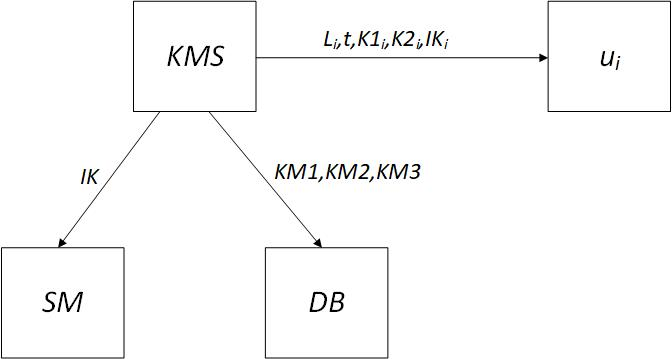
\includegraphics[width=200pt]{papers/ppiot/images/KeyDist}
    \caption{Deployment key configurations.}
    \label{fig:keydist}
\end{figure}

\section{Data protection}
\label{dataprotection}
We are considering a model where a huge number of IoT devices regularly uploads new data items to the storage server $SM$. According requirement R5, this shall be possible to do without the need for any security sessions. A straight forward way to handle this is to use an object security model. Object security for the IETF session protocol for constraint devices, CoAP \cite{rfc7252} is standardized in the Object Security for Constrained RESTful Environment (OSCORE) standard \cite{RFC8613}. While this is a very resource efficient protocol, it gives not identity anonymity of the sending party. Furthermore, it is closely aligned to the CoAP protocol. In our scenario, we do \emph{not} want to just protect the data from the sending device to the storage manager end-to-end as offered by OSCORE, but actually \emph{also} data storage at the $SR$ as we considering a model where the attacker might have access to both the $SM$ and $SR$. Hence, we have defined a new privacy preserving object security format. The format is completely independent of the actual bearer protocol but can for instance be transferred over CoAP as standard non-protected payload. Below, we describe the encryption procedure (at the device side) and format as well as decryption procedures (database side of the system).

\subsection{Data encryption procedure}
\label{dataprotection:encryption}
Each devices regularly uploads data to the $SM$ in protected format. We suggest the following encryption procedure:
\begin{enumerate}
    \item $u_i$ uses a good random source to generate two random values: $n_1,n_2$.
    \item $u_i$ selects uniformly and at random an index, $l_{ip}$, from the set $L_i$.
    \item $u_i$ selects a first encryption IV, $IV1 = l_{ip}||n_1$.
    \item $u_i$ selects a second encryption IV, $IV2 = t||n_2$.
    \item $u_i$ encrypt the data item, $d$ to obtain a first ciphertext: $c1 = \text{E}_{K1_i}(IV1,d)$.
    \item $u_i$ encrypt $IV1$ to obtain a second ciphertext: $c2= \text{E}_{K2_i}(IV2,IV1)$.
    \item $u_i$ calculates a inner message authentication cod: $h_{in} = \text{MAC}_{IK_i}(IV2||c2||c1)$
    \item $u_i$ calculates a message authentication code over $IV2||c2||c1||h_{in}$: $h_o = \text{MAC}_{IK}(IV2||c2||c1||h_{in})$.
\end{enumerate}
Finally, $u_i$ sends the protected message, $IV2||c2||c1||h_{in}||h_o$, using an arbitrary communication channel to $SM$, which verifies the message authentication tag, $h_o$, and if the verification is successful, stores $IV2||c2||c1||h_{in}$ for future processing at $SR$. The protected message format is illustrated in Figure \ref{fig:protection}.
\begin{figure}[ht]
    \centering
    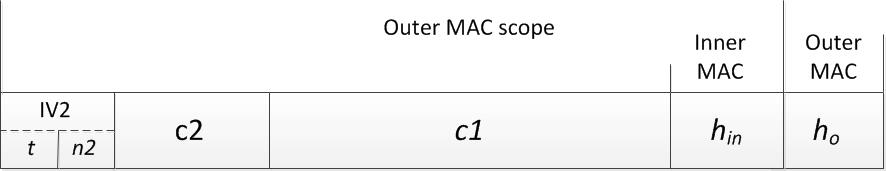
\includegraphics[width=200pt]{papers/ppiot/images/ProtectionFormat}
    \caption{Protection format.}
    \label{fig:protection}
\end{figure}
\subsection{Data decryption procedure}
\label{dataprotection:decryption}
According to the system scenario we are considering, the $DB$ is responsible for decryption protected IoT data items on $SR$ and to index them for future processing. However, there is no need for the $DB$ to re-encrypt the data items but they can be kept in protected form on the $SR$ as the decryption process is quick as we show below.
The decryption procedure is as follows:
\begin{enumerate}
    \item $DB$ fetches a protected data item from the $SR$:  $IV2||c2||c1|h_{in}$
    \item $DB$ extracts $t$ from $IV2$.
    \item $DB$ calculates: $K2_t = \text{PRF}(KM2,t)$.
    \item $DB$ decrypts $c2$ to obtain: $IV1 = D_{KM2}(IV2,c2)$.
    \item $DB$ extracts $l = r||c$ from $IV1$.
    \item $DB$ obtains the true device index $i$ through decryption: $i = \text{D}_{KM3}(r,c)$ (corresponding to the index encryption in (\ref{keygen:devindex})).
    \item $DB$ calculates $KI_i = \text{PRF}(KM1,"MAC"||i)$.
     \item $DB$ calculates $h'_{in} = \text{MAC}_{IK_i}(IV2||c2||c1)$. If $h'_{in}$ equals $h_{in}$, the data, the item is accepted, otherwise it is rejected.
    \item $DB$ calculates $K1_i = \text{PRF}(KM1,"Enc"||i)$.
    \item $DB$ uses $K1_i$ and $IV1$ to obtain the clear text data item $d' = \text{D}_{K1_i}(IV1,c1)$ .
    
    
\end{enumerate}

\graphicspath{{analysis/images/}}
\section{Security analysis}
\label{secanalysis}
Next, we analysis the security properties of the proposed protection scheme. The focus of the analysis is the security requirements R1, R2 and R4 (see Section \ref{requirements:requirements}). R3 is here omitted as this is a pure back-end system property that can be achieved by state-of-the-art protection mechanisms.
\newtheorem{prop}{Proposition}
\begin{prop}
\label{analysis:confidentiality}
 Given that the symmetric encryption algorithm, E, provides confidentiality protection and for a non-compromised IoT unit encryption key, $K1_i$, the proposed scheme provides confidentiality protection.
\end{prop}
\begin{proof}
The worst case attack scenario given the prerequisites in the proposition, is when the attacker has full knowledge of $IV1$ but no knowledge of the key $K1_i$. In this case, for all different data items, $d_0$, $d_1$ and corresponding encrypted cipher texts, $c_0=E_{K1_i}(IV1,d_0), c_1=E_{K1_i}(IV1,d_1)$, the distinguish probability (\ref{eq:confidentiality}) equals the very same probability for the used symmetric encryption algorithm. This proofs the Proposition.
\end{proof}
According to our attacker model, adversary knowledge of $K1_i$ only happens when the IoT unit $u_i$ is compromised. However, if this IoT input is compromised, the attacker will have access to all data protected by this particular unit anyway, and our any protection scheme is not useful. Hence, we conclude that the proposed scheme give good protection for the data for the \textit{majority} of the IoT units. This is true as we assume it will only be feasible for an attacker to compromise a limited number of the IoT units in the system.
\begin{prop}
\label{analysis:integrity}
For a non-compromised IoT unit $u_i$, given that the chosen function $MAC$ is $(q,l,\epsilon)$ unforgeable, the proposed scheme provides data item integrity if: $l $ is greater than the maximum number of bits in $d$, $q$ is larger than the maximum number of messages produced by $u_i$ and $\epsilon$ is negligible.
\end{prop}
\begin{proof}
A data item produced by $u_i$ is first encrypted into $c_1$, which in turn is protected by $(q,l,\epsilon)$ unforgeable $MAC$ using key $IK_i$. Hence, if $IK_i$ is not compromised. $d$ is (indirectly) protected by a $(q,l,\epsilon)$ unforgeable $MAC$. Furthermore, it follows from the assumptions in the Proposition that $l$ is greater than the maximum number of bits in $d$, that $\epsilon $ is negligible and that $q >$ maximum number of messages produced by $u_i$. Hence, the Proposition follows directly from Definition \ref{integrity}
\end{proof}
The same reasoning around IoT encryption key compromise, $K1_i$ for unit $u_i$ applies also to integrity key compromise, $IK_i$ of the unit. Hence the scheme also give good integrity data protection for the \textit{majority} of the IoT units. 
\begin{prop}
\label{analysis:kanonymity}
 Given that the symmetric encryption algorithm, E, provides confidentiality protection and for a non-compromised group encryption key, $K2_t$, the proposed protection scheme provides k-anonymity.
\end{prop}
\begin{proof}
 In the IDA game, the attacker, for chosen messages $m \in M$ observes $q$ different evaluations of  $f_{K2_i}(u_i,m) = c1,c2,h_{in}$ together with $u_i$. Here we have, $c2 = \text{E}_{K2_t}(IV2,IV1)$, where $IV1$ is an encrypted index, $l_{ip}$ randomly mapped from random selections of $u_i$. As the input to the calculation of $c1,c2$, and consequently, also the input to the calculation of $h_{in}$ are depending on random numbers $n1,n2$, these values are randomly distributed on the encryption and MAC spaces independently of the chosen message, $m$. Next, the attacker can choose any previously observed value $t$ (part if $IV1$) and corresponding previously observed message $m$ and get the corresponding, $v' = c1',c2',h'_{in}$. If $c1',c2'$ equals a previous observed $c1,c2$, the attacker wins with probability one as he/she can choose, in this case, a previously observed, $h_{in}$. This probability is less than  the probability that just $c2'$ equals a previously observed crypto text $c2$.  Due to the random selections of $n1$, $n2$, $l_{ip}$ by the IoT unis, observation of a previously observed $c2$ happens with probability less than $2^{\text{log}_2(q) - \text{log}_2(w) - \text{log}_2(||n1||) -\text{log}_2(||n2||)} = \epsilon$. If, $c2'$ does \textit{not} equal a previously observed crypto text, an attacker that tries to decrypt $c2'$ to obtain $l'$, can in the worst case map $l'$ to a particular user $u'$. However, since, the group key, $K2_2$, not is known to the attacker, and the encryption algorithm gives confidentiality protection, it follows from (\ref{eq:confidentiality}) that this attack game succeeds with a probability of at most $\epsilon(n)$. Hence, in case of that $c2'$ does not equal a previous observed crypto text, a random selection of $u' \in U_t$ (as $t$ is known to the attacker) gives the best chance of success. As $|U_t| \leq k, Pr(u'= \hat{u}) \leq 1/k $, this gives an overall probability of success $\epsilon +(1-\epsilon)\cdot(1/k) \approx 1/k$.
\end{proof}
This proposition shows that as long as the group unique key not is leaked, the scheme provided k-anonymity. However, as the size of a group can be rather large  (equal to $t$), compromise of this key cannot be excluded in same cases. However, even in this situation, the proposed scheme gives some anonymity guarantees as showed by the following proposition.

Now, denote by $\text{Bin}(q; k/|U|)$ the binomial distribution, i.e. with the density function:
\begin{eqnarray*}
P(X=j) = 
\begin{pmatrix}
q \\
j
\end{pmatrix}
(k/|U|)^j(1-(k/|U)^{q-j}.
\end{eqnarray*}
Then let: 
\[
 \text{BSum}[(k,w),\text{Bin}(q;k/|U|)] =
 \]
 \[
\begin{cases}
\sum\limits_{j=0}^{q} \frac{1}{k-\frac{j}{w}} P(X=j), & \text{if} \ q \leq w(k-1) \\
\sum\limits_{j=0}^{w(k-1)}\!\frac{1}{k-\frac{j}{w}} P(X=j) + \!\!\!\!\!\! \sum\limits_{w(k-1)+1}^q \!\!\!\!\!P(X=j) & \!\text{otherwise}
\end{cases}
\]
\begin{prop}
\label{analysis:idunforgeable}
Assume, $q < w|U|$, then the proposed protection scheme is $(q,q/(w|U|+(1-q/w|U|)\text{BSum}[(k,w),\text{Bin}(q;k/|U|)])$ unforgeable. 
\end{prop}
\begin{proof}
A worst case scenario is an attacker with full knowledge of $K2_t$ for all possible choices of $t$. Under these circumstance, the attacker can ask for $q$ number of different values $f_{L_i}(u_i) = IV1 = (l_{ip},n_1)$  together with $u_i$ (outer encryption and message selection can be disregarded in this case). Next, in the game, the attacker observes $v' = f_{L_i}(\hat{u})$. If $v'$ has been previously observed, the attacker wins the game with probability one. For each data protection occasion at most $q$ different $(l_{i}, u_i)$ pairs have been recorded by the attacker. Furthermore, as $\hat{u}$ is selected at random \textit{and} the index $l_{i}$ is chosen at random among the $w$ different available indices, the probability that $v'$ has previously been observed is then less than $q/(w|U|)$. This follows from the fact that the total number of $(l_{i}, u_i)$ pairs equals $w|U|$ and that maximum $q$ unique different pairs have been observed by the attacker. If $v$ has not previously been observed, an optimal game strategy for the attacker is to choose $u'$ as the identity of the least number of previously observed identities in $\{v'\}$ belonging to set $U_t$. Denote this number by $z$.  Furthermore, assume, the number of observed elements $U_t$ equals $j$. Then the probability of successful attack for this strategy is less than $(w-z)/(wk-j) \leq w/(wk-j) = 1/(k-(j/w))$, if $j\leq w(k-1)$. While if $j>w(k-1)$, the probability is less than 1. The probability of having $j$ elements in the previous observation belong to set $U_t$ is due to the random selections, equal to the binomial density function. Hence, by taking the expected value of $1/(k-(j/w))$ for the binomial distribution and summing up to the number of observations, $q$, we end up with the an expected probability which is less than $\text{BSum}[(k,w),\text{Bin}(q;k/|U|)]$.
\end{proof}
This proposition is proved under the scenario that all keys $K2_t$ are leaked which is typically not possible to achieve for a limited attacker. Even under this circumstance, as the proposition shows, the scheme still provides a level of anonymity. The strength of the anonymity can be tuned using the size of the parameter $w$. However, a larger $w$ comes with higher IoT non-volatile memory cost. It is important to also notice though, that unforgeability is made under the worst chosen message attack scenario and in many practical situations it will not be possible for an attacker to gather enough number of clear text $(l_{i}, u_i)$ pairs for protected data items. Especially, it is hard for an attacker to get knowledge of the real identity behind an observed index value, $l_i$. 

\graphicspath{{Performance/images/}}
\label{peranalysis}
\section{Performance figures}

\subsection{Proof of Concept Implementation}
To evaluate the feasibility of our suggested privacy protection scheme, we have implemented a proof of concept system. We have developed an application for IoT devices that generate data items that are encrypted according to our proposed scheme. These encrypted data items are then sent to a $SM$ where $h_0$ is verified and then to $DM$ where they are decrypted. The $KMS$ is left out of scope. Our IoT application for data encryption is written in C and is running on Contiki-NG\footnote{\url{https://github.com/contiki-ng/contiki-ng/}}, an open source operating system for constrained IoT devices. 
The IoT devices that we have run our tests on are Zolertia Firefly\footnote{\url{https://zolertia.io/product/firefly/}} development boards based on the Texas Instruments cc2538\cite{instruments2015cc2538} system on chip. The cc2538 features an ARM Cortex-M3 clocked at 32MHz, with 32KB of RAM and 512KB of ROM.  The back-end system that consists of the $SM$ and $DM$ is written in Java and running on a Linux host, specifically a  Lenovo T460 laptop with an Intel Core i7-6600U CPU clocked at 2.60 GHz. 
We have chosen the following algorithms in our implementation:
\begin{itemize}
    \item   $E_K(m)\, \& \, D_K(c)$  AES128-CTR  
    \item  $PRF(K,a)$  HKDF-SHA256 
    \item  $MAC_K(m)$  HMAC-SHA256
\end{itemize}
The AES128-CTR algorithm and the SHA265 algorithm used was implemented in software on the IoT devices. The encrypted device indexes $l_{ip}$ was selected to be 8 Bytes long, the IoT device was provisioned with $|L_i| = 10$. The encrypted data items were transferred from the IoT device to the back-end using CoAP \cite{rfc7252}. The transfer of data is left out-of-scope for these performance measurements since our proposed scheme is independent of underlying protocols. 

\subsection{IoT Device Performance}
As discussed in Section \ref{introduction}, energy is a major concern for IoT devices, especially those that rely on battery power. CPU-time is also limited on constrained systems. Both these metrics are important when considering solutions aimed at IoT devices. We have measured the time taken to encrypt data items. To investigate how the performance depends of the size of time data item $d$ we have tested the following sizes of $d$; 1,8,16,32 and 64 bytes. For each size of data items $d$ we did the encryption 500 times. The times were measured and the energy consumption was calculated from the times and the stated power consumption in the cc2538 data-sheet. The results can be seen in Figure \ref{fig:iot_performance}. %The measured times show very little deviation, this is because the Contiki-NG operating system is non-preemptive, all threads will execute until complete, no task can be interrupted. This together with the lack of any cache and branch-prediction makes the execution times very uniform.
\begin{figure}[H]
    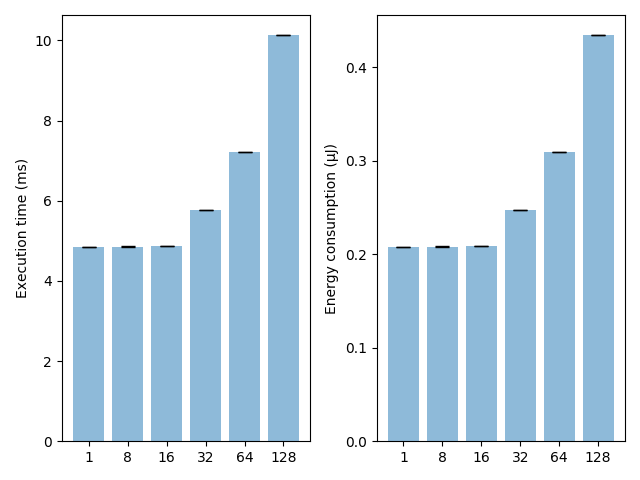
\includegraphics[width=\linewidth]{papers/ppiot/images/iot_bar_plot.png}
    \caption{Execution time and energy consumption for encrypting data. The graphs show the mean of the of the execution times and derived energy consumption with a 95\% confidence interval.}
    \label{fig:iot_performance}
\end{figure}

\subsection{Back End Server Performance}
To evaluate how the throughput of a back-end server would be affected by the privacy protection scheme we have measured the time taken to verify $h_0$, furthermore we have measured the time taken to decrypt the data item $d$ including verifying $h_{in}$. The performance was measured running in a single thread. We have measured the for different encrypted payloads $d$; 1,8,16,32 and 64 bytes. The times for a single payload size $d$ varies considerably, we have made 2000 measurements for each payload size. The times can be seen in Figure \ref{fig:java_performance}. 
%When observing the measurements one can see that the execution times vary, we believe this is because of the non-deterministic performance of the Java Runtime Environment and the underlying operating system.
\begin{figure}[H]
    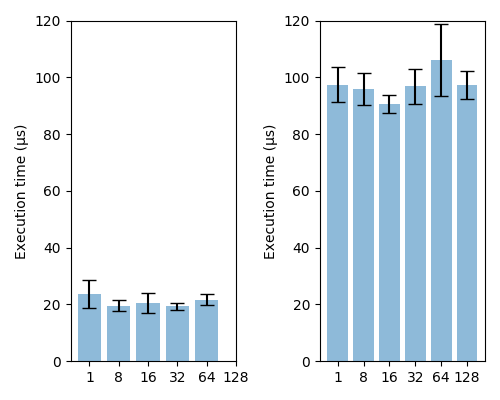
\includegraphics[width=\linewidth]{papers/ppiot/images/java_bar_plot.png}
    \caption{Execution time, left graph shows verifying $h_0$, right graph decryption of encrypted $d$ and verifying $h_{in}$. The graphs show the means of the of the execution times with a 95\% confidence interval.}
    \label{fig:java_performance}
\end{figure}
To give an estimation of the throughput of our solution we use conservative numbers of $50\mu s$ for verifying $h_0$ and $150\mu s$ for decrypting and verifying $d$, this gives us a total time of $200\mu s$ for one data item. The total throughput for one core would then be 5000 data items per second.

\subsection{Memory usage on IoT devices}
IoT devices have limited resources in terms of memory, any scheme developed for such a device must keep this in mind. Here we present numbers for the memory utilization of our implementation. The total utilization of ROM was 2344 Bytes and 426 Bytes of RAM. This was used by SHA256 836 Bytes, HMAC-SHA256 114 Bytes, AES128-CTR 1026 Bytes, Encryption Function 368 Bytes. The RAM was divided between 144 Bytes of keys in RAM and buffers for the encryption process of 282 Bytes. This is manageable amounts of memory needed for such a scheme. If the cipher and hash algorithms would be hardware-accelerated the memory usage would be even lower.


\section{Related work}
\label{relatedwork}
Privacy is a major concern in the IoT paradigm\cite{perera2015big}. People and devices are surrounded by billions of IoT devices gathering zettabytes of data, device manufacturers still do not pay enough attention to privacy while IoT devices are not capable of handling costly solutions to preserve privacy. 

%In  they provide good notions and terminology for iot data privacty, identity data temporal and location etc...

When discussing privacy it is worthwhile to note that there are several types of privacy\cite{porambage2016quest}. Data privacy aims at preserving privacy by not revealing data created or owned by an entity, while identity privacy aims at protecting the identity of a user or entity. There are also the notion of spatial or location privacy, here the goal is to hide or obfuscate the location of the user or entity. This is mostly relevant in the domain of mobile devices\cite{chen2017robustness}  but can also have an impact for V2X networks and IoT networks. Location privacy is not directly related to the work we present in this paper. 

The principle of k-anonymity was first introduced 1998 by  Pierangela and Sweeney and has been extensively use as an annonymization measure in different privacy settings \cite{Sweeney2002}. An overview of different k-anonymity approaches is given in \cite{Ayala2014}. In our paper we adapt the k-anonymity principle in an IoT identity privacy setting.

General privacy-preserving solutions include differential privacy \cite{DworkMNS06}, homomorphic encryption \cite{gentry2009fully}\cite{naehrig2011can}, and secure multi-party computation \cite{bringer2013privacy}. %\cite{lindell2005secure}
Another general line of research which is relevant to the IoT paradigm is privacy-preserving aggregation of time-series data \cite{JoyeL13} \cite{BenhamoudaJL16} \cite{EmuraKOS18} \cite{ShiCRCS11}. Many sensors periodically generate data on e.g. temperature and sends it to a server for analysis. A recent summary of these more general problems can be found in \cite{shan2018practical}. Bista et. al. provides a survey of privacy-preserving data aggregation protocols for wireless sensor networks (WSN). In \cite{conti2009privacy}, a scheme for anonymous data transfer using only symmetric key operations is presented. The paper introduces the notion of twin-keys, keys negotiated between two nodes where the nodes does not know the identity of the other node in the pair. This provides anonymity of individual devices when doing data aggregation.

However, all these approaches are so far elusive for the IoT paradigm: they are too computationally costly for resource-constrained IoT devices.  

Going into solutions aimed specifically at IoT it is worth to note that IoT includes a wide spectrum of devices and technology. While different solutions have been proposed for IoT, the work has primarily aimed at data privacy. 
One application of IoT is smart electricity meters (SM), a device measures the electricity consumption at a customer. The measurements needs to be forwarded to the utility-company for billing, but the customers privacy needs to be considered. Learning when the customer utilizes electricity can reveal the users habits. In \cite{Silva:2017:SPP:3019612.3019795} Silva et. al. presents a scheme for data aggregation in smart electricity meters using an Intel SGX enclave to perform the data aggregation while providing end user privacy. 

In \cite{zhang2018data} Zhang et. al. survey the entire fields of security and privacy in edge computing. They give an overview of edge computing, list issues regarding security and privacy, list requirements. They also provide descriptions of key technologies: Identity-based encryption, Attribute-based encryption, proxy re-encryption, homomorphic encryption and searchable encryption. They give an overview of state-of-the-art solutions for data confidentiality, data integrity, privacy preserving and more. They have a section on both data-privacy and identity-privacy, they list some proposed schemes for identity privacy.

Identity privacy has been researched primarily in the fields of Mobile Communications and Vehicular Networks. in the field of Mobile Communications Khan et. al. presents their scheme for dynamic credential generation in \cite{khan2013enhanced}, they also provide an extensive overview of work in the field. Their proposed scheme uses public-key encryption, which makes their proposed solution too computationally intensive for our use-case.

In the field of Vehicular Networks Identity privacy is important\cite{whyte2013security} since a vehicle broadcasting the the identity of the vehicle or driver would enable location tracking of the vehicle or driver. Most of the identity privacy issues of Vehicular networks are solved by pseudonyms, the vehicle is issued with a public-key pair that is periodically changed. Much research has been done on how to improve these schemes \cite{lin2013}, \cite{lin2008tsvc}. However, since the basis of these systems are based on public-key cryptography they are to computationally complex for constrained IoT devices. 

\section{Conclusion and future work}
\label{conclusion}
In this paper, we presented a novel principle for IoT identity protection when using pure symmetric key based data confidentiality and integrity protection. The symmetric key approach has big advantages compare to a public key-based approach as it allows fast analytic processing directly on the protected data items on cloud resources. Identity privacy in this context has not been treated in the literature before and we provided basic security definitions. Using these definition, we presented a novel \textit{combined} identity protection, encryption and integrity protection scheme for IoT data objects. The suggested protection scheme gives not full privacy in all adversary scenarios but, as we view it, gives a fair trade-off between identity protection and complexity. In particular, the proposed schemes uses a two layered protection approach where an ''outer'' protection schemes gives k-anonymity based on symmetric keys shared by several IoT units. If such key would be compromised, an ''inner'' identity protection schemes based on random encryption gives a second level of privacy defense. The security analysis we presented, shows that a reasonable level of identity privacy is achieved with this approach, as long as the adversary not has access to a large number of compromised IoT units or a large number of mappings between specific protected data items and the IoT identity behind the data items. Furthermore, by tuning the protection parameters, increased privacy can be achieved thought the price of more memory usage at the IoT device side. Our proof of concept implementation verifies that the proposed principle indeed offers both low energy consumption encryption at the IoT side as well as fast decryption at the analytic engine side. In future work, we intend to make a full-scale implementation of the approach on IoT data from an industrial control system. In this extended system trial, we will also integrate the solution with a selected set of state-of-the art analytic engines. It is also left for future work to investigate if even more efficient identity privacy preserving schemes for symmetric encryption can be constructed.

{\raggedright
        \printbibliography[segment=\therefsegment,heading=subbibliography]
}


\fi

\ifpaperIII
\newrefsegment
\addtolength{\apa}{2cm}
\fancyhead[RE]{\paperref{ch:oscore}: \paperIIItitle}
\chapter[\paperIIItitle]{\texorpdfstring{%
                \paperIIItitle}{%
                \paperIIItitle}}

\label{ch:oscore}
\paperRemark{This is the full version of the paper below.
        This version contains an extended background description, and a more detailed motivation behind choices in the implementation as well as evaluation.
        \paperIIIref}
{i

\section{Introduction}
\label{s:introduction}

The Internet of Things (IoT) refers to a networked scenario where all connectable devices are reachable over the Internet and can communicate with each other. This has led to many new application scenarios, e.g. smart buildings, plant and home automation, smart electricity grids and smart transportation.

In such deployments, several IoT devices, also called \emph{nodes}, are units with limited resources such as memory, computing power and energy (if they are battery-powered). Having constrained resources results in constrained network segments, e.g. due to lossy channels and limited bandwidth \cite{rfc7228}. In order to cope with this, resource-constrained nodes tend to adopt an asynchronous and intermittent communication model, i.e. they handle network traffic according to sending/receiving timeslots. To save energy, nodes can go offline (\emph{sleep}), between two active timeslots, considerably extending their lifetime.

To manage these limitations, \emph{proxies} are used as intermediaries to enable access to server nodes that are not always online, by caching and forwarding requests.  With this in mind, the Constrained Application Protocol (CoAP) \cite{rfc7252} has been developed with support for proxying functionality, and is now a de-facto standard application-layer protocol for IoT. CoAP is a RESTful protocol, REST being an acronym for Representational State Transfer \cite{fielding2000architectural}. The REST model considers a Client and a Server as communicating parties, where the Client sends a Request to the Server, which replies by sending a Response. Based on the intended operation to perform, CoAP Requests can be of different types, e.g. GET, PUT, POST, FETCH, PATCH and DELETE.

Most applications require secure communications between client and server nodes. To this end, the CoAP specification \cite{rfc7252} considers Datagram Transport Layer Security (DTLS) \cite{rfc6347} as the only method to achieve secure communication for CoAP. In particular, DTLS establishes a secure channel at the \emph{transport layer} over unreliable datagram protocols such as UDP, and hence provides hop-by-hop security by protecting CoAP messages in their entirety. Due to proxies not being able to read encrypted CoAP messages, a DTLS channel must terminate at a proxy, so that the proxy can read the data needed for proxying functionality. As a consequence, a single DTLS channel cannot be established directly between the Client and the Server. Instead, a first secure channel has to be established between a Client node and the proxy, and then a second secure channel has to be established between the proxy and the Server node. This in turn results in the two following issues and limitations.

First, it is necessary to perform a double security processing of CoAP messages, as the proxy has to decrypt a message received on the client DTLS channel, and then re-encrypt the same message for delivery on the server DTLS channel, which impacts performance. Second, the proxy is necessarily required to be trusted, as it is able to fully access the CoAP messages. Mandating trust in proxies and the service providers operating them to such an extent results in unnecessary exposure of data.

This paper presents Object Security for Constrained RESTful Environments (OSCORE), an \emph{application-layer} approach for message protection based on \emph{object security} that efficiently overcomes these issues. To this end, OSCORE selectively protects certain parts of the CoAP messages at the application layer, providing \emph{end-to-end} secure communication between client and server nodes. In particular, some parts of CoAP messages can be encrypted, while other parts can be only authenticated and integrity-protected. This makes it possible to deploy non-trusted proxies, which are still able to perform their intended tasks. Furthermore, this greatly mitigates privacy threats otherwise possible for proxies to exploit, thus preserving the personal sphere of human users related to the information exchanged and the operations performed by the communicating endpoints. OSCORE has been recently standardized in the Internet Engineering Task Force (IETF) \cite{cite:oscoap}.

We have implemented OSCORE for the Contiki-NG OS \footnote{\url{https://github.com/contiki-ng/contiki-ng/wiki}}, and tested it on the resource-constrained platform Zolertia Firefly \footnote{\url{https://zolertia.io/product/firefly}} equipped with the CC2538 system-on-a-chip \footnote{\url{http://www.ti.com/lit/ds/symlink/cc2538.pdf}}. Then we used our implementation to experimentally evaluate OSCORE, considering a CoAP client and a resource-constrained CoAP server that securely communicate through a CoAP proxy.

In particular, we evaluated performance in terms of memory and CPU usage as well as energy consumption on the server side, and Round Trip Time experienced on the Client side. In our evaluation, we compared OSCORE performance against both an insecure baseline scenario using plain CoAP and a secure scenario using CoAP over DTLS. Our results show that OSCORE outperforms DTLS in terms of message overhead, round-trip time and energy efficiency, while still allowing a (non-trusted) proxy to perform its intended operations. To the best of our knowledge, this paper provides the first comprehensive performance evaluation of the standardized OSCORE protocol on a real IoT device, including a comparison against DTLS.

The rest of the paper is organized as follows. Section \ref{sec:related} presents the related work. Section \ref{sec:back} describes background technologies and concepts. Section \ref{sec:obj} provides the motivation behind this work, while Section \ref{sec:protocol} presents OSCORE. Section \ref{s:payloadoverhead} analyzes the overhead introduced by OSCORE, while Section \ref{sec:measure} describes our experimental setup. In Section \ref{sec:results}, we present and discuss experimental results. Finally, in Section \ref{sec:conclude}, we draw our conclusions.

\section{Related Work}
\label{sec:related}

A number of approaches have been proposed for optimizing channel security protocols to constrained devices and networks. In particular, Raza \textit{et al.} adapted DTLS to improve performance for resource constrained devices by using header compression mechanisms from 6LoWPAN  \cite{cite:lithe}. This reduces message overhead, thus increasing energy efficiency and avoiding fragmentation. Raza \textit{et al.} also proposed to use Next Header Compression, so that IP Security can be adapted to resource constrained devices \cite{cite:razaipsec}. Hummen \textit{et al.} considered the viability of certificate-based DTLS and suggested to offload parts of the DTLS handshake to trusted gateways \cite{cite:hummen}. Sethi \textit{et al.} proposed a similar approach, providing also end-to-end data integrity and with particular focus on performance of public-key cryptography for resource constrained devices \cite{cite:sethi}.

All these approaches aim at reducing message overhead and ultimately improving performance of constrained devices and networks. However, none of them aims at providing end-to-end secure communication between client and server devices, in the presence of intermediate (untrusted) entities such as proxies. For example, one article has been presented by Van den Abeele \emph{et al.} in \cite{s17071609} where the authors identify the problem with DTLS and proxies. The aim of their work is to offload the work of the constrained servers, however they do not achieve end-to-end security through proxies.

To achieve end-to-end security, other schemes based on object security have been proposed. One approach which is similar to OSCORE is OSCAR \cite{cite:OSCAR}, which also provides object security for the Internet of Things, but with a focus on access control. Besides, the object security format in OSCAR is designed for protection of \textit{publish-subscribe} communications, rather than client-server \textit{end-to-end} communications. That is, OSCAR considers a \textit{many-requests-one-response} communication model, where many requests can be answered with the same response. Instead, OSCORE considers a \textit{one-request-one-response} communication model, where request and response are strictly associated.

Work has also been done on how to protect CoAP messages. In \cite{nguyen2015}, the authors present an alternative scheme relying on object security, aimed at providing integrity-protection and authentication of CoAP messages. However, unlike OSCORE, the proposed scheme does not leverage standard efficient building blocks such as CBOR \cite{rfc7049} and COSE \cite{rfc8152}, and requires the addition of several new CoAP options, thus resulting in a considerable overhead for each secure message. Moreover, the usage of the HMAC-SHA256 algorithm for message integrity protection results in $32$ byte Message Authentication Codes (MACs) for each protected message, which is a further significant overhead for constrained devices.

Another end-to-end security scheme for CoAP was proposed in \cite{ukil2014lightweight}. This relies on a new CoAP option and uses AES-CCM-128 for encryption and authentication. However, this scheme does not leverage CBOR and COSE either, with consequent overhead due to inefficient encoding. Also, unlike OSCORE, it protects only the message payload, without securing CoAP options and header fields.

Finally, in \cite{musaddiq2018}, the authors present an evaluation of OSCORE only. That is, they show how offloading AES-CCM encryption and decryption operations to hardware significantly improves performance, especially as to energy efficiency. However, the evaluation does not include a performance comparison against any alternative security solution, e.g. DTLS. Also, it is based on their implementation of an old version of OSCORE, well before its standardization as \cite{cite:oscoap}. 

This paper provides an experimental evaluation of the OSCORE standard on a real IoT device, and includes a comparison against both an insecure baseline scenario using plain CoAP and a secure scenario using CoAP over DTLS. To the best of our knowledge, no such comprehensive contribution has been done before.

\section{Background}
\label{sec:back}

This section introduces background concepts referred to throughout the paper.

\subsection{Channel Security and Object Security }
\emph{Channel security} refers to the transmission of data over a secure channel \cite{rfc3552}. This can be negotiated at the data link, network or transport layer in the protocol stack, through a specific establishment protocol. Most important, a secure channel handles data agnostically, i.e. it has no knowledge of the conveyed secure data.

\emph{Object security} refers to protection mechanisms for data objects, as an alternative to secure channels \cite{rfc3552}. Instead of relying on a communication protocol at a lower layer to provide message protection, applications also take care of protecting and verifying data objects of their own generated messages.

\subsection{CoAP}\label{coap}
The approach presented in this paper is aimed at the Constrained Application Protocol (CoAP) \cite{rfc7252}, which is an application layer web transfer protocol, designed for resource constrained devices and networks. CoAP typically runs on top of UDP \cite{rfc768}, is not session-based and can handle loss or delayed delivery of messages. Also, it features an asynchronous messaging model and has native support for proxying. 

A CoAP message is divided into header and payload. The CoAP header may include a number of \emph{options}, which follow a Type-Length-Value scheme and are used to control various functions of the protocol. For example, options can be used to instruct a proxy on how to handle messages, specify for how long a message is valid, or even indicate message fragmentation at the application layer.


\subsection{CBOR and COSE}
\label{sec:cose}
\emph{Concise Binary Object Representation} (CBOR) \cite{rfc7049} is a data encoding format designed to handle binary data, with the primary goal of achieving very small parser code size, and the secondary goal to achieve small message size. \emph{CBOR Object Signing and Encryption} (COSE) \cite{rfc8152} specifies how to perform encryption, signing and Message Authentication Code (MAC) operations on CBOR data and to encode the result in CBOR.

\subsection{DTLS}
\label{ss:background-dtls}
DTLS \cite{rfc6347} is an Internet standard providing channel security at the \emph{transport layer} to protect communications over unreliable datagram protocols, such as UDP. That is, security is ensured hop-by-hop, i.e. between two nodes that are adjacent transport-layer hops. DTLS is a close copy of the TLS protocol \cite{rfc5246} and provides equivalent security guarantees, i.e. it prevents tampering, eavesdropping and message forgery. In particular, DTLS is adapted for use over UDP \cite{rfc768} instead of TCP \cite{rfc793}, which is important for constrained devices and networks relying on UDP as a connectionless transport protocol. The original CoAP specification \cite{rfc7252} indicates DTLS as the only security mechanism to protect the exchange of CoAP messages.

Two communicating devices initially use the DTLS \textit{Handshake} protocol to exchange network information and cryptographic key material for later message protection. In particular, one device acts as \textit{client}, while the other acts as \textit{server}. The default \textit{Handshake} relies on certificates, but extensions based on symmetric pre-shared keys \cite{rfc4279} or on raw public keys \cite{rfc7250} are often preferred in constrained applications. Once completed the \textit{Handshake} and established a secure session, client and server start exchanging data protected through the negotiated key material.

Secure communication is then carried out using the DTLS \textit{Record} protocol, which provides security and reliability of message transfers. This works as an encapsulating protocol that transports data and connection state information among the two communicating parties. The \textit{Record} layer header conveys information including data type, sequence number, and length of the message content.

\section{Motivation and Objectives}
\label{sec:obj}

A significant part of IoT devices are resource-constrained, with many even being battery powered. It is therefore important to limit resource consumption, especially in terms of energy, to achieve a long device lifetime and acceptable performance. As introduced in Section \ref{s:introduction}, energy performance may rely on device \emph{sleeping}, which in turn leads to an asynchronous communication model. In order to still provide a well functioning service, it is thus necessary to schedule requests to sleeping nodes with the help of proxies, used as intermediaries between clients and servers.

\begin{figure}[!ht]
\centering
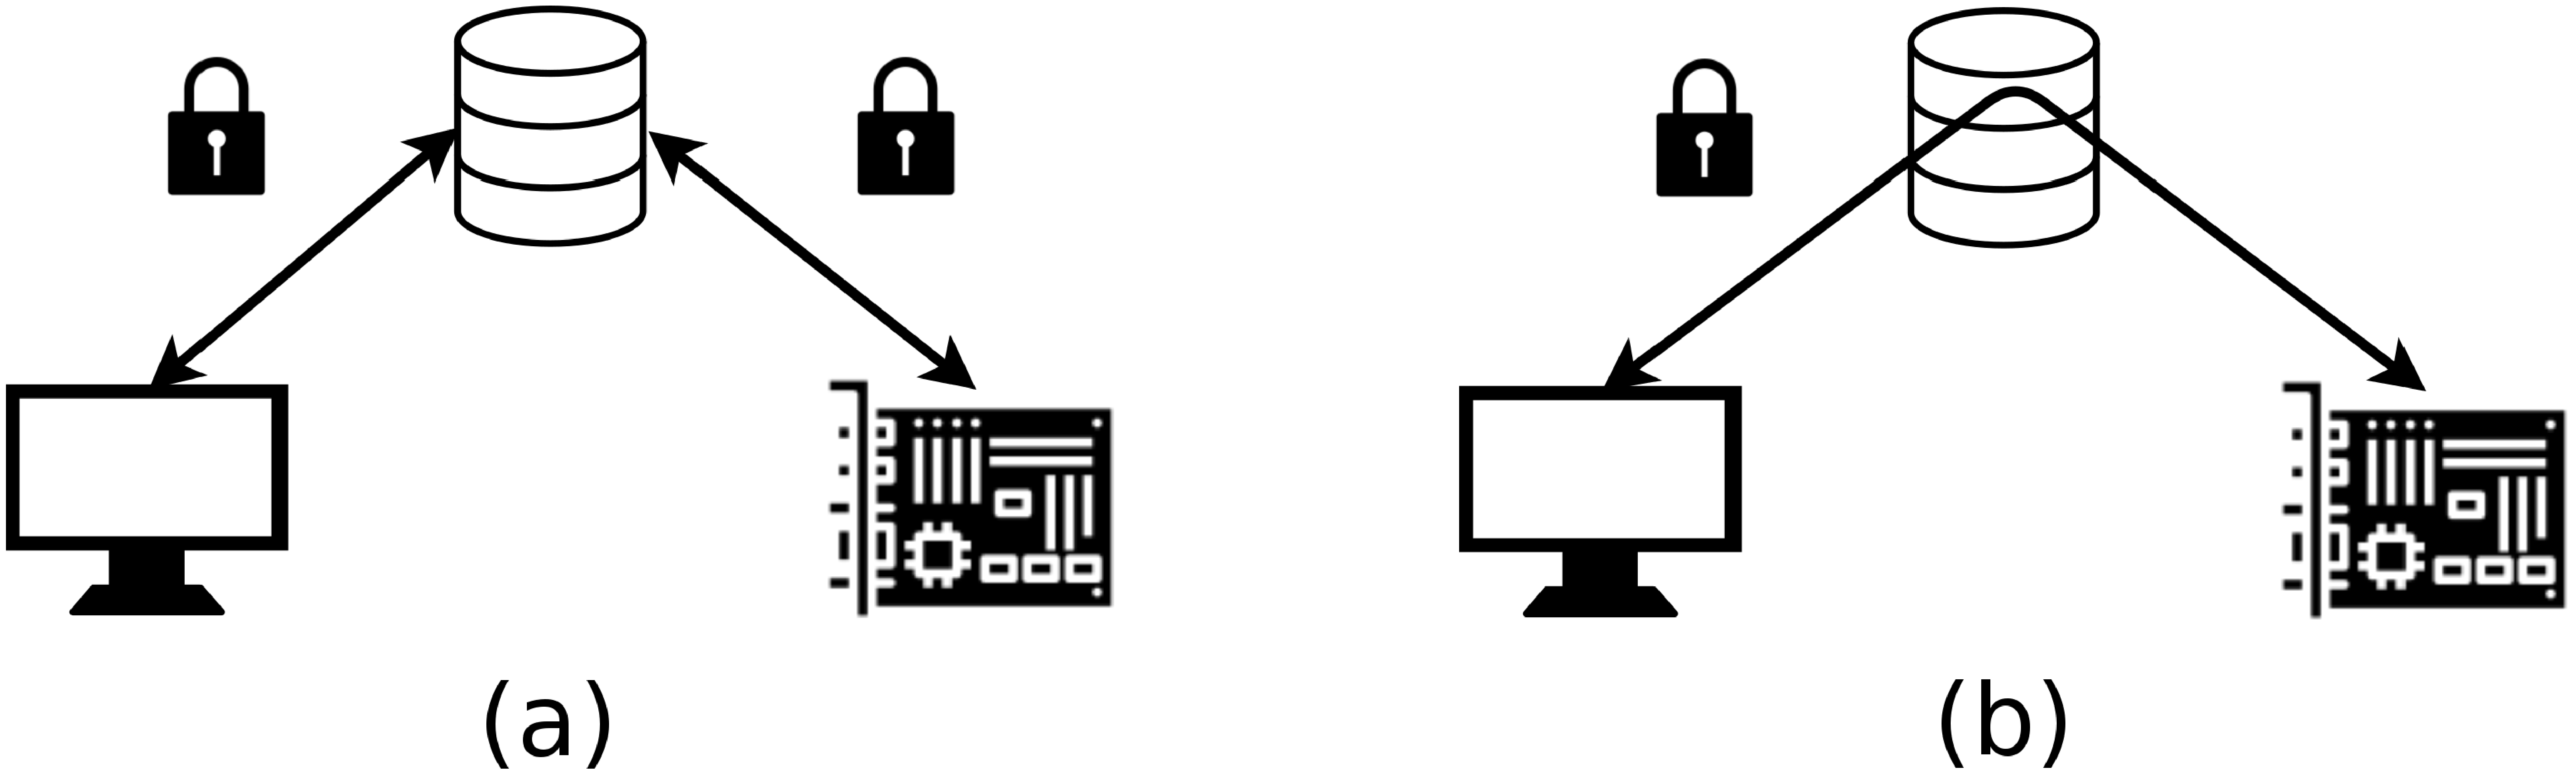
\includegraphics[width=0.8\textwidth]{papers/oscore/images/secure_comm}
\caption{Hop-by-hop vs. end-to-end security}
\label{fig:secure_comm}
\end{figure}

The original CoAP specification \cite{rfc7252} indicates DTLS \cite{rfc6347} as the only method to achieve secure communication for CoAP. This in turn means that, when a proxy is deployed between a client and server, message protection is enforced \emph{hop-by-hop} between client, proxies and server, as shown in Figure \ref{fig:secure_comm}(a). Thus, in the presence of an intermediary proxy, DTLS cannot provide \emph{end-to-end} secure communication between a client and server node. Instead, a first secure channel has to be established between the client and the proxy, and a second secure channel has to be established between the proxy and the server. This in turn results in the issues and limitations discussed in Section \ref{s:introduction}, i.e. the double security processing on the proxy as well as having to fully trust the proxy.

Figure \ref{fig:secure_comm}(b) shows the alternative \emph{end-to-end} security approach, where a client and a server rely on a two-way secure communication context. This approach essentially consists in tunneling channel security through the proxy, and hence successfully overcomes the two limitations discussed before. However, in order to be practically deployable and functional, a solution based on end-to-end security must not prevent proxies to correctly perform their intended functionalities, especially the caching of CoAP requests. Therefore it must be possible to \emph{selectively} protect different parts of a same CoAP message in different ways, i.e. some encrypted, others only integrity protected and finally some parts fully accessible by the proxy.

This flexibility can be achieved by using \emph{object security}, so that applications can choose which parts of an outgoing message have to be integrity-protected, encrypted, or both. Note that protecting only the CoAP payload is not sufficient against attacks such as changing the REST \emph{Code} field in the CoAP header, e.g. from \emph{GET} to \emph{DELETE}, which tricks the server into deleting a resource instead of just returning its value. 

The above motivates a need for lightweight end-to-end security with preserved proxying functionality, and has in turn led to the design of OSCORE, an application-layer protocol based on object security, which fulfills these requirements.


\section{Protocol description}
\label{sec:protocol}

%The code size of the cn-cbor library \cite{cite:cn-cbor} (constrained device
%CBOR) is roughly 1.4KB for an embedded ARM-Cortex-M3 platform.

\label{sec:oscoap}
This section describes Object Security for Constrained RESTful Environments (OSCORE). For the reader's convenience and due to space constraints, we only present the main features, while a complete description is available at \cite{cite:oscoap}.  OSCORE provides message confidentiality, integrity and reordering/replay protection, as well as a weak freshness protection through sequence numbers for CoAP messages. To this end, OSCORE transforms an \textit{unprotected CoAP message} into a \textit{protected CoAP message}. A protected CoAP message includes the newly defined \emph{OSCORE option} \cite{cite:oscoap}, which signals the usage of OSCORE to protect the message, as well as an encrypted COSE object \cite{rfc8152} in the CoAP payload. 

OSCORE is designed for providing end-to-end security between two CoAP endpoints, while preventing intermediaries to alter or access any message field that is not related to their intended operations. The security concerns not only the actual payload of the original CoAP message, but also all the fully protected CoAP options, the original request and response REST code, as well as parts of the URI to resources targeted in request messages (see Section \ref{ss:proxy_func}). 

To be able to use OSCORE, the following two criteria must be fulfilled. First, the two CoAP endpoints are required to support CBOR and COSE (see Section \ref{sec:cose}), as well as the specific \emph{HMAC-based Key Derivation Function} (HKDF) and \emph{Authenticated Encryption with Associated Data} (AEAD) algorithms they want to use for key derivation and authenticated encryption, respectively. This assumption is often already fulfilled in the vast majority of IoT applications using CoAP. Second, the two CoAP endpoints are required to have an OSCORE security context (see Section \ref{sec:con}), or the necessary information and keying material to derive it. While this has to happen in a secure and authenticated way, and some suitable approaches are proposed in \cite{cite:coseecdh}\cite{cite:oscoreprofile}, OSCORE is not tied to any particular approach for context establishment, and further details are out of the scope of this paper.

\subsection{The security context}
\label{sec:con}
OSCORE uses parameters and keying material included in an OSCORE \emph{security context}, and used to perform encryption and integrity protection operations. For this reason, every pair of communication endpoints, i.e. a CoAP client and a CoAP server, share the same security context.

The security context consists of three parts:  a \emph{Sender} part, a \emph{Recipient} part and a \emph{Common} part. The \emph{Sender} part is used to protect outgoing messages (i.e. requests on the client and responses on the server). The \emph{Recipient} part is used to verify incoming protected messages (i.e. requests on the server and responses on the client). Finally, the \emph{Common} part contains shared data. This division is illustrated in Figure \ref{fig:security_context}. An instance of a security context is present as a copy on the client and server, containing the same data values. However, as can be seen in Figure \ref{fig:security_context}, the sender and recipient parts are mirrored, so that the sender part of the server corresponds to the recipient part of the client, and vice versa.
\begin{figure}[ht]
    \centering
     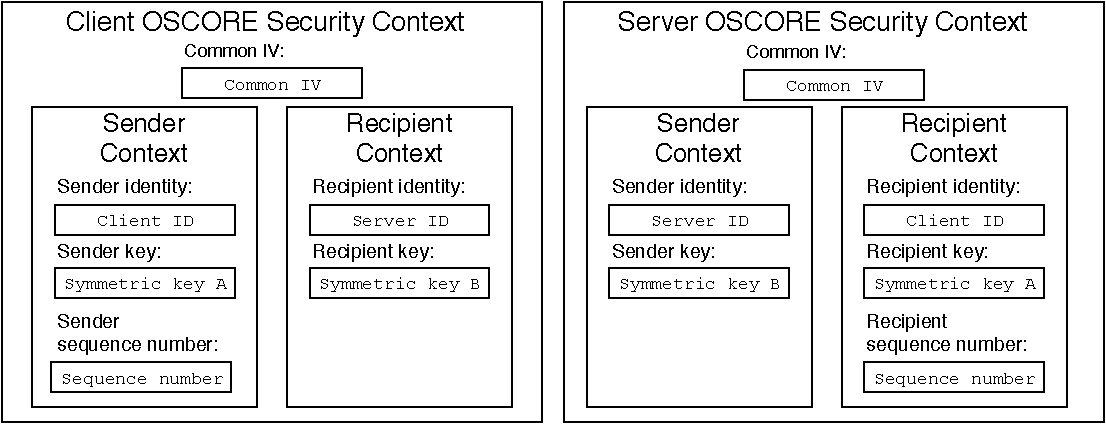
\includegraphics[width=\textwidth]{papers/oscore/images/OSCORE_contexts.pdf}
    \caption{OSCORE Security Contexts for a Client and Server pair showing only the fields used during operation.}
    \label{fig:security_context}
\end{figure}{}

In more detail, the \emph{Common} part includes: i) an identifier of the AEAD algorithm used to encrypt and authenticate exchanged messages; ii) an identifier of the HMAC-based key derivation function used to derive keys and initialization vectors (IVs); iii) the \emph{Master Secret}, a random byte string used to derive keys and IVs; iv) the \emph{Master Salt}, an optional byte string used with the Master Secret to derive the keys and IVs; v) a Context ID, used to identify the Common Context and to derive keys and IVs; vi) a Common IV to generate AEAD nonces.

The \emph{Sender} part includes: i) a \emph{Sender ID}, a byte string identifying the \emph{Sender} part of the security context; ii) a \emph{Sender Key}, the symmetric key to protect outgoing messages; iii) a \emph{Sequence Number}, used for nonce generation to protect outgoing messages, and for replay protection of incoming messages (see Section \ref{sec:repl}).

The \emph{Recipient} part includes: i) a \emph{Recipient ID}, a byte string identifying the \emph{Recipient} part of the security context; ii) a \emph{Recipient Key}, the symmetric key to decrypt incoming messages; iii) a \emph{Replay Window} to verify freshness of incoming messages on the CoAP server (see Section \ref{sec:repl}).

The combination of Context ID, Sender ID, Master Secret and Master Salt must be unique for each communicating pair of Client and Server. This ensures unique keys and nonces for the AEAD. Further details on establishing Sender/Recipient IDs and the ensuring their uniqueness are out of the scope of OSCORE and of this paper.

\subsection{Protecting the CoAP message}
\label{ss:COSE_object}

Different parts in a CoAP message are protected in different ways. That is, \textit{Confidential data}, which should neither be read or altered by a proxy, are both encrypted and integrity protected. \textit{Static data}, which should be readable but not changed, are integrity protected but not encrypted. \textit{Dynamic data}, which a proxy should be able to modify, are not protected. Finally, there are also \textit{Mutually known data}, which the sender and receiver have agreed upon before exchanging messages. These data are part of the input to the integrity protection process, to ensure that the two communicating endpoints behave correctly and possibly detect anomalies. However, they are never sent as both parties already know them.

Figure \ref{fig:prot_struct} shows a comparison between an unprotected CoAP message and the resulting OSCORE-protected CoAP message. We can see that sensitive parts of a message are encrypted, e.g. some options and the payload, while others are left unencrypted, e.g. some options and some fields of the CoAP header. The encrypted content is placed into the payload of the protected message.

\begin{figure*}
\centering
   \begin{subfigure}[b]{\textwidth}
   \centering
     \begin{bytefield}[bitwidth=.9em]{32}
        %\bitheader{0-31} \\
         \bitbox{5}{Version} & \bitbox{4}{Type} & \bitbox{7}{Token Length} & \bitbox{8}{CoAP-Code} & \bitbox{8}{Message ID} \\
         \wordbox{1}{Token} \\
        \bitbox{9}{Option A} & \bitbox{6}{Option B} & \bitbox{6}{Option C} & \bitbox{11}{Option D} \\
        \bitbox{8}{Payload delimiter} & \bitbox{24}{CoAP-Payload}  \\
    \end{bytefield}
    \caption{CoAP message format.}
    \label{fig:coap-header}
   \end{subfigure}
  \newline
  \newline
    \begin{subfigure}[b]{\textwidth}
    \centering
    \begin{bytefield}[bitwidth=.9em]{32}
        %\bitheader{0-31} \\
         \bitbox{5}{Version} & \bitbox{4}{Type} & \bitbox{7}{Token Length} & \bitbox{8}{CoAP-Code} & \bitbox{8}{Message ID} \\
         \wordbox{1}{Token} \\
        %\bitbox{6}{Option B} & \bitbox{8}{11111111} & \bitbox[tlr]{24}{}  \\
        \bitbox{6}{Option B} & \bitbox{8}{OSCORE Option} & \bitbox{8}{Payload delimiter} & \bitbox[tlr]{10}{}  \\
        \wordbox[blr]{1}{Encrypted\{\footnotesize{Option A, Option C, Option D, CoAP-Code, CoAP-Payload}\} $+$ AEAD-tag} \\
    \end{bytefield}
    \caption{OSCORE message format.}
    \label{fig:oscore-header}
  \end{subfigure}
  \caption{Message layout for unprotected and protected CoAP messages.}
  \label{fig:prot_struct}
\end{figure*}

The actual protection process takes as input an unprotected CoAP message and produces a protected OSCORE message as follows.

\noindent
\textbf{1)} The confidential data are enclosed into a \textit{COSE object} \cite{rfc8152}. These include the REST code of the original CoAP message, a subset of the CoAP options, and the CoAP payload (if present). The CoAP options considered at this step are the ones not relevant for operations of intermediary (proxy) units.

\noindent
\textbf{2)} The static fields of the CoAP header and static proxy-readable CoAP options needs to be authenticated and integrity protected, but not to encrypted. This set of data composes the \emph{Additional Authenticated Data} (AAD).

\noindent
\textbf{3)} The COSE object is finalized, by encrypting and integrity protecting the data it encloses, while only integrity protecting the AAD. To this end, the Sender Key and the Sender Sequence Number from the Sender Context are used. The resulting \emph{ciphertext} and \emph{AEAD-tag} is included in the \emph{Message Content} field of the COSE Object.

\noindent
\textbf{4)} The COSE object is used as payload of the protected CoAP message, and any encrypted options are removed from the CoAP message. The original REST code is replaced with POST (2.04) for a CoAP request (response), or with FETCH (2.05) for a CoAP request (response) using the \emph{Observe} mechanism \cite{rfc7641}.

An analogous reverse process is performed upon receiving a protected message, together with anti-replay checks (see Section \ref{sec:repl}). To decrypt the protected message, the recipient CoAP endpoint uses the Recipient Key from its own Recipient Context associated to the message originator.




\subsection{Proxy functionalities and data protection}
\label{ss:proxy_func}
Building on the previous sections, we can now describe how OSCORE handles proxying of encrypted messages. OSCORE is designed to uniquely bind each request to the corresponding response, thus preventing proxies from serving cached responses to clients different from the one originating the request.

%OSCORE supports forward proxy functionalities, which affects the parts of CoAP messages accessed by forward proxies. That is, not all the data in the CoAP message can be encrypted, as some must remain readable to allow proxies to operate correctly. However, it is mostly possible to integrity protect such data.

As previously stated, OSCORE cannot encrypt entire CoAP messages. An example of static data in a CoAP message which can not be encrypted but should be integrity protected is the \emph{Version} field of the CoAP header. This field has to remain readable, so that the receiver endpoint knows how to process an incoming message, but should be integrity protected to prevent future version-based attacks.

The \emph{Token} field of the CoAP header also has to remain readable, as it is used for binding each request to the corresponding response. However, unlike the \emph{Version} field, the \emph{Token} field cannot be integrity protected, as it can be modified by proxies, when a message traverses the network.

\subsection{Replay protection}
\label{sec:repl}
OSCORE provides protection against replay and message reordering attacks. To this end, both the client and server store a sequence number and a replay window as part of the security context (see Section \ref{sec:con}) and including said sequence number in every outgoing request, before incrementing it by 1. Upon receiving a protected request, the server verifies that the conveyed sequence number was not received before. To correctly handle messages received out of order, OSCORE relies on a sliding window of sequence numbers, where the server accepts only messages with sequence number greater than the lower bound of the replay window. In such a case, the server updates its replay window accordingly. Otherwise, the server considers the message to be a retransmission and discards it.

\section{Evaluation of Payload and Network Overhead}
\label{s:payloadoverhead}
To aid reasoning and facilitate further discussion in the next sections, we have analyzed the payload overhead in bytes, as introduced by DTLS and OSCORE with respect to plain CoAP. To ensure a fair comparison, we have considered the same AEAD cipher for both DTLS and OSCORE, namely AES-128-CCM-8. Tables \ref{fig:overhead_dtls} and \ref{fig:overhead_oscore} show the overhead of the two different protocols. The entry "AEAD Tag" refers to the resulting Integrity Check Value produced by the AEAD cipher.

\begin{table*}[ht]

\captionsetup[subtable]{position = below}
\captionsetup[table]{position=top}
\begin{subtable}{0.3\linewidth}
\centering
\begin{tabular}{l|l}
Type    & 1  \\
Version & 2  \\
Epoch           & 2  \\
Sequence Number & 6  \\
Length          & 2  \\
AEAD Tag        & 8  \\ \hline
Total overhead           & 21
\end{tabular}
\caption{Overhead of a DTLS-record layer message (bytes).}
\label{fig:overhead_dtls}
\end{subtable}%
\hspace*{2em}
\begin{subtable}{0.3\linewidth}
\centering
\begin{tabular}{l|l|l}
                     & Request & Response \\
OSCORE Option Byte   & 1    & 1\\
OSCORE Flag Byte     & 1    & -\\
Partial IV           & 0-5  & -\\
Kid                  & 0-7  & -\\
CoAP Code            & 1    & 1\\
Payload Marker       & 1    & 1\\
AEAD Tag             & 8    &  8\\ \hline
Total overhead       & 12-24 & 11
\end{tabular}
\caption{Overhead of an OSCORE message (bytes).}
\label{fig:overhead_oscore}

\end{subtable}
\caption{Payload overhead for DTLS 1.2 and OSCORE.}
\end{table*}

As we can see in Table \ref{fig:overhead_dtls}, DTLS displays a fixed overhead of $21$ bytes, which is equal for both requests and responses. This results in a total overhead of $42$ bytes for a full message exchange. Note that, as defined in the DTLS profile for IoT in \cite{rfc7925} (Appendix B), devices using DTLS are expected to additionally include an $8$-byte explicit nonce to the DTLS header. This would result in an overhead of $29$ bytes per message, i.e. of $58$ bytes for each two-way message exchange.

In OSCORE, the overhead can vary, due to the following reasons. First, the "Partial IV" field in the OSCORE option includes the message sequence number, whose value is incremented and size grows over time as Requests are transmitted, up to a maximum size of $5$ bytes. Second, the "Kid" field (Key Id) in the OSCORE option is immutably set by the user during early configuration, with possible sizes ranging between $0$ (empty Key Id) and $7$ bytes. 

With reference to Table \ref{fig:overhead_oscore}, we can see that, as long as the Key Id is chosen to have a length of maximum $4$ bytes, OSCORE will display the same or lower overhead for all Requests. Note that a Key Id of maximum $2$ bytes is expected to be the practical choice for most applications using OSCORE. Furthermore, OSCORE Responses omit a number of implicit fields in the OSCORE option, and thus showing a smaller fixed overhead of $11$ bytes. Note that, unlike DTLS, OSCORE has a (much) smaller overhead for responses than requests. Assuming a high-value Partial IV of $5$ bytes and a Key Id of $2$ bytes, this would result in an overhead of $19$ bytes per request message and of $11$ bytes per response message, i.e. of $30$ bytes for a two-way message exchange.

Also, an application relying on IEEE 802.15.4 typically displays an effective data rate (i.e. excluding headers, CRCs and control packets) of about $8.4$ kbit/s (out of $250$ kbit/s). However, as shown by Latr\'{e} \emph{et al.}, IEEE 802.15.4 networks can actually achieve a throughput of about $140$ kbit/s, even if acknowledgement frames are transmitted \cite{latre:2005}. Using these numbers together with the energy consumption numbers stated in the CC2538 datasheet\footnote{\url{http://www.ti.com/lit/ds/symlink/cc2538.pdf}}, we get the numbers shown in Table \ref{tab:overhead}.
\begin{table}[ht]
\center

\begin{tabular}{l|ll|ll}
         & \multicolumn{2}{l}{Time (ms)} & \multicolumn{2}{l}{Energy ($\mu J$)} \\ 
         & DTLS         & OSCORE         & DTLS                   & OSCORE                  \\ \hline
Request  & 1.2          & 1.086          & 95.04                  & 71.676                  \\
Response & 1.2          & 0.628          & 79.2                   & 49.738                  \\
Exchange & 2.4          & 1.714          & 174.24                 & 121.414                

\end{tabular}
\caption{Overhead in transmission time and energy consumption for a cc2538 server receiving and sending DTLS and OSCORE messages.}
\label{tab:overhead}
\end{table}

\section{Experimental Evaluation Method}
\label{sec:measure}

To evaluate the feasibility and convenience of OSCORE, we developed a prototype implementation for resource-constrained CoAP servers. This section presents the conducted experiments which evaluates the performance of OSCORE. We chose to evaluate OSCORE against both plain CoAP and CoAP secured with DTLS since CoAP recommends DTLS as a security mechanism. The plain CoAP scenario, namely "COAP", acts as a baseline comparison for the DTLS-based scenario, namely "COAPS", and for the OSCORE-based scenario, namely "OSCORE". We show that, even with no particular optimizations, OSCORE displays an affordable overhead, and outperforms DTLS in terms of resource utilization and energy consumption on the server side, as well as responsiveness perceived on the client side.

%TODO, perhaps we should change the picture to include the proxy.
% M.T. Agree. Also, "Radio" can be renamed to "IEEE 802.15.4 link"
\begin{figure}[!htbp]
\centering
%images are free to use without attribution (https://iconmonstr.com/cpu-2-eps/)
\begin{tikzpicture}[scale=1,every node/.style={outer sep=.2cm}]
\node (client) at (0,0) {
\includegraphics[height=1cm]{papers/oscore/images/iconmonstr-laptop-6.pdf}};
\node[right = 1.7cm of client] (proxy)  {
\includegraphics[height=1cm]{papers/oscore/images/iconmonstr-laptop-6.pdf}};
\node[right = 1.7cm of proxy] (router) {
\includegraphics[height=.8cm]{papers/oscore/images/iconmonstr-radio-tower-1.pdf}};
\node[right = 1.7cm of router] (server) {
\includegraphics[height=1cm]{papers/oscore/images/iconmonstr-cpu-2.pdf}};


\node[above = -0.3cm of client] (client-h) {\scriptsize Client};
\node[above = -0.3cm of proxy] (proxy-h) {\scriptsize Proxy};
\node[above = -0.2cm of router] (router-h) {\scriptsize Border Router};
\node[above = -0.3cm of server] (server-h) {\scriptsize Server};

\draw[<->]([xshift=0cm]client.east) -- ([xshift=-0cm]proxy.west) node [midway, above] (usb) {\tiny IP};
\draw[<->]([xshift=0cm]proxy.east) -- ([xshift=-0cm]router.west) node [midway, above] (usb) { \tiny USB};
\draw[<->]([xshift=0cm]router.east) -- ([xshift=-0cm]server.west) node [midway, above] (radio) { \tiny IEEE 802.15.4};

\end{tikzpicture}
\caption[Test set-up]{Experimental test scenario.}
\label{fig:setup}
\end{figure}

For our experiments, we considered the test scenario in Figure \ref{fig:setup}, which consists of a CoAP client, a CoAP proxy and a CoAP server. The client (C) and the proxy (P) were implemented using an extended version of the Java library Californium/Scandium \footnote{\url{http://www.eclipse.org/californium}}, which provides both CoAP and DTLS. The client and the proxy ran as two distinct processes on a same commodity PC. To enable communication between P and the server (S), we relied on a dedicated border router (BR) device. In particular, both BR and S were resource-constrained Zolertia Firefly boards \footnote{\url{https://zolertia.io/product/firefly}}, and ran the Contiki-NG OS \footnote{\url{https://github.com/contiki-ng/contiki-ng/wiki}} together with an extended version of the Erbium library providing the communication stack. The Firefly boards are based on the CC2538 chipset and equipped with 512 KB of ROM, 32 KB of RAM, a 32 MHz ARM Cortex-M3 CPU, and an IEEE 802.15.4 \cite{IEEEStd802.15.4} radio interface.

We considered and compared three different test cases: "COAP", "COAPS" and "OSCORE". In all three test cases, P acts as CoAP proxy and relays CoAP requests from C to S, as well as corresponding CoAP responses from S to C. More specifically, the three test cases were defined as follows.

\noindent
$\bullet$ \textbf{"COAP"}. The "COAP" test case considered plain CoAP communication, with no security provided.

\noindent
$\bullet$ \textbf{"COAPS"}. The "COAPS" test case considered CoAP communication with the addition of DTLS 1.2, providing hop-by-hop secure communication. DTLS was configured with a first secure channel between C and P, and a second secure channel between P and S. Both DTLS channels used the DTLS ciphersuite TLS\_PSK\_WITH\_AES\_128\_CCM\_8 \cite{rfc6655}.

\noindent
$\bullet$ \textbf{"OSCORE"}. The "OSCORE" test case considered CoAP communication with the addition of OSCORE, providing end-to-end secure communication between C and S, as described in Section \ref{sec:protocol}.

Note that neither "COAPS" nor "OSCORE" relied on hardware acceleration for cryptographic operations, and that "COAP" does not make use of cryptography.

In all three test cases, the client sent POST requests addressed to a dedicated target resource at the server S. Also, S was configured to reply to each such request by sending a response with the same payload size. The client was pre-configured in order to skip the resource discovery process.

In the considered setup, the server did not rely on the Radio Duty Cycling mechanism provided by Contiki for switching off the node's radio interface if not in use \footnote{\url{https://github.com/contiki-os/contiki/wiki/Radio-duty-cycling}}. In the "COAPS" and "OSCORE" test cases, the involved parties had already established a security association which enabled a secure message exchange. That is, the completion of the DTLS handshake, as well as the establishment of OSCORE security contexts, were out of scope for this paper and our performance evaluation, which focused on the (secure) exchange of messages.

For each test case, we performed separate experiments. During a given experiment, the payload size of every CoAP message was either $1$, $16$, $32$, $48$, $64$, $80$, $96$, $112$ or $128$ bytes. For each listed payload size, we performed $500$ message exchanges between the client and the server, through the proxy. In all the test cases, we performed the following measurements: i) Responsiveness as experienced by C for a message exchange with S; ii) CPU usage by the server; iii) Memory usage by the server, i.e. RAM and ROM; iv) Radio usage by the server; and v) Energy usage by the server. In particular, we performed the measurements as follows.

\noindent
\textbf{Responsiveness}. We evaluated the Round Trip Time (RTT), as experienced by the client when performing a full Request-Response exchange. The statistical significance of these results were verified with the method of paired t-tests.

\noindent
\textbf{CPU usage}. We measured the execution time needed to process both incoming messages from a client and  outgoing response messages. For the "COAPS" and "OSCORE" test cases, this includes decryption and integrity verification of incoming messages, as well as encryption of outgoing messages. Paired t-tests were used for verification of statistical significance.

\noindent
\textbf{Memory usage}. The static memory utilization was determined by using the GNU utility \emph{size}. Since Contiki-NG does not use dynamic memory allocation on the heap, dynamic memory utilization is limited to the stack. Hence, in our experiments, we used the \textit{stack painting} painting technique, where a known value is written to all addresses of the stack part of the memory. After the experiments, the number of bytes that had been overwritten by the program execution were counted.

\noindent
\textbf{Radio usage}. We have measured the time needed by the server to receive and transmit messages using \emph{Energest}, a Contiki-NG utility for monitoring system utilization. Energest makes it possible to measure the time intervals where the CPU has been active, or where the radio interface has been active either in reception mode (RX) or transmission mode (TX). Furthermore, Energest has been proven to enable an accurate estimation of energy consumption, while increasing the computing time only of the $0.7\%$ \cite{energest}.

\noindent
\textbf{Energy usage}. We measured the energy consumed at the server, both by the CPU, and by the radio interface in transmission and reception mode. Each measurement was computed as the product between the overall related time collected by Energest, and the power consumption of the related hardware component as documented in the respective manuals\footnote{\url{https://zolertia.io/product/firefly}}\footnote{\url{http://www.ti.com/lit/ds/symlink/cc2538.pdf}}.

\section{Results and Discussion}
\label{sec:results}

This section presents and discusses the results of our experiments, with reference to the test cases and scenario described in Section \ref{sec:measure}. The data presented here represent the average for a single message from a sample set of $500$ messages.

\subsection{Responsiveness}
The top graph in Figure \ref{fig:rtt} shows the average RTT experienced by the client for different payload sizes, with the different curves showing the three different test cases. The bottom graph shows the calculated difference in mean response time between OSCORE and COAPS, with error-bars showing the standard deviation.

\begin{figure}[ht]
\centering
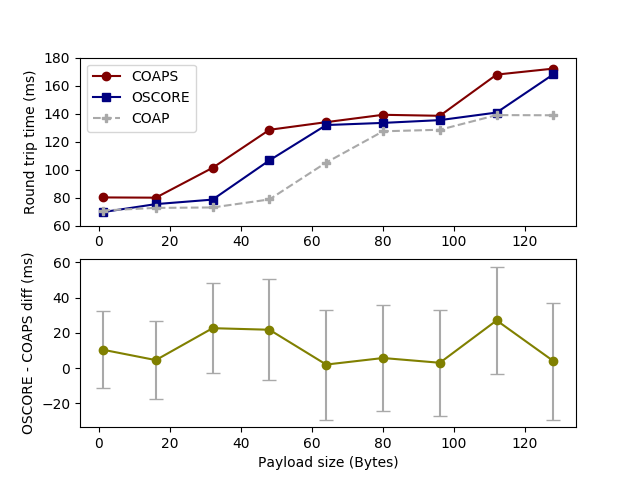
\includegraphics[width=0.8\textwidth]{papers/oscore/images/rtt.png}
\caption[RTT measurements]{Measurement of responsiveness comparing RTT between COAP, COAPS and OSCORE. }
\label{fig:rtt}
\end{figure}

Table \ref{tab:tstat} shows the statistical significance (t-statistics and p-values) for the values in the bottom graph in Figure \ref{fig:rtt}. For each payload size, the statistics are derived using paired t-tests, comparing response time sample populations.

\begin{table}[ht]
\centering
\caption {Statistical significance for RTT, (t-statistics and p-values)} \label{tab:title} 
\small\addtolength{\tabcolsep}{-2pt}
\begin{tabular}{c|c|c|c|c|c|c|c|c|c}
Payload \\ (Bytes)  & 1    & 16   & 32   & 48   & 64   & 80   & 96   & 112  & 128  \\ \hline
                  t & 7.8  & 3.2  & 14.5 & 12.2 & 1.0  & 3.0  & 1.7  & 13.8 & 1.9  \\ 
                  p & 0.0 & 0.0 & 0.0 & 0.0    & 0.30 & 0.0 & 0.09 & 0.0 & 0.06
\end{tabular}
\label{tab:tstat}
\end{table}

As it can be seen in Figure \ref{fig:rtt}, there is a notable difference in the mean response time between the protocols, with OSCORE being more efficient than COAPS for all payload sizes. The statistical significance of the difference, see Table \ref{tab:tstat}, is strong for most packet sizes, achieving a 99\% confidence interval. However, for 64, 96 and 128 bytes payload, statistical significance is not achieved. This is likely due to a large variance in transfer time on the IEEE 802.15.4 network. Overall, the lines in the top graph of Figure \ref{fig:rtt} resemble a staircase. Further investigation showed that this is due to package fragmentation.

\begin{figure}
\centering
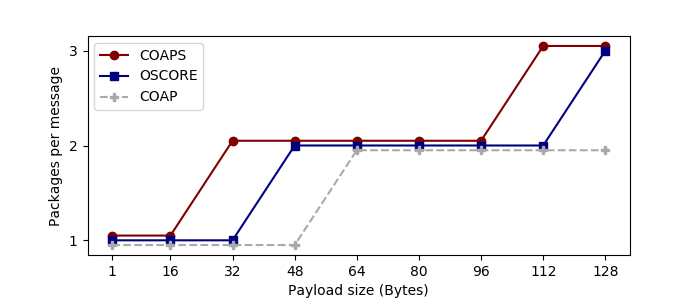
\includegraphics[width=1.0\textwidth]{papers/oscore/images/frags.png}
\caption[Fragmentation measurements]{number of packages needed to transport a single message. }
\label{fig:frag}
\end{figure}

Figure \ref{fig:frag} shows the number of packages needed to transport one message for the different protocols and payloads. We can see that the biggest possible payload that can be carried in a single frame has a different size in the three scenarios, with COAP being able to fit the most data into a single frame and COAPS the least. This is because the total header sizes for the used protocols vary between the COAP, OSCORE and COAPS scenarios, i.e. $76$, $90$ and $105$ bytes, respectively. The Maximum Transmission Unit for a IEEE 802.15.4 network is 127 bytes.

\subsection{CPU usage}
Figure \ref{fig:parse} and Figure \ref{fig:serialize} show the CPU time for processing incoming and outgoing COAP, COAPS and OSCORE messages. The left graphs show the total CPU time for the different protocols, including cryptographic operations. The right graphs show the CPU time excluding cryptographic operations.
\begin{figure}[ht]
\begin{subfigure}{1.0\textwidth}
\centering
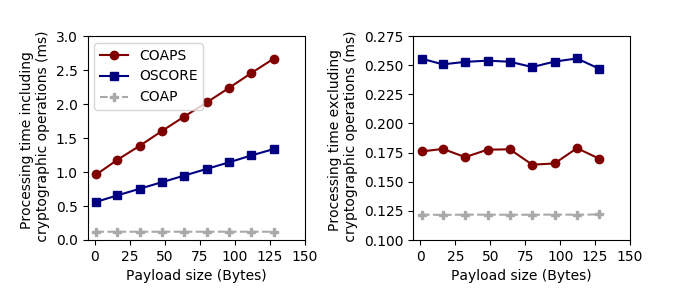
\includegraphics[width=1.0\textwidth]{papers/oscore/images/proc.png}
\caption[Processing measurements]{Measurement of CPU time when processing incoming messages with COAP, COAPS and OSCORE. }
\label{fig:parse}
\end{subfigure}

\begin{subfigure}[ht]{1.0\textwidth}
\centering
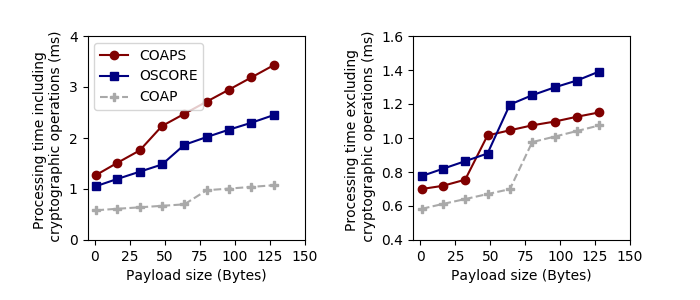
\includegraphics[width=1.0\textwidth]{papers/oscore/images/serialize.png}
\caption[Processing measurements]{Measurement of CPU time when processing outgoing messages with COAP, COAPS and OSCORE. }
\label{fig:serialize}
\end{subfigure}
\end{figure}

In particular, Figure \ref{fig:parse} shows the CPU-time for processing incoming messages. The left graph shows the total CPU-time for processing incoming messages with COAPS, OSCORE and COAP. The graph shows that OSCORE is faster than COAPS when processing incoming messages, for all message sizes. In the right graph of Figure \ref{fig:parse}, we show the CPU-time for processing incoming messages excluding the CPU-time spent for decryption. Here we see that OSCORE takes longer time than COAPS for all message sizes.

Similarly, Figure \ref{fig:serialize} shows the CPU-time for processing outgoing messages. The left graph shows the total CPU-time for processing outgoing messages with COAPS, OSCORE and COAP. Where cryptographic operations are taken into account, OSCORE is faster than COAPS when processing outgoing messages, for all messages sizes. In the right graph of Figure \ref{fig:serialize}, we show the CPU-time for processing outgoing messages excluding the CPU-time spent for encryption. Again, here we see that OSCORE takes longer time than COAPS for all message sizes. 

The observed difference between the right and left side of the graphs is due to the following reasons. Other than the actual encryption/decryption processing of messages, OSCORE is slower than DTLS due to: i) a more complex handling of OSCORE security contexts (i.e. retrieval and update), compared to the handling of DTLS sessions; ii) a more complex preparation of a protected OSCORE message from an original CoAP message and vice versa (see Section \ref{sec:protocol}), compared to the preparation of a protected DTLS record from an original CoAP message and vice versa. However, when also cryptographic operations are taken into account, OSCORE outperforms DTLS as more efficient in protecting/unprotecting handled messages. Ultimately, OSCORE achieves this result especially by leveraging a more efficient implementation of the AES-CCM algorithm.

The results in both Figure \ref{fig:parse} and Figure \ref{fig:serialize} are verified for statistical significance with 99\% confidence interval using a paired t-test. The results of these experiments show that the CPU performance for both protocols hinges on a fast cipher implementation. In these experiments we used software implementations of AES128-CCM. Hardware acceleration of the encryption will increase the performance of both OSCORE and COAPS.

\subsection{Memory usage}
Figure \ref{fig:memory} shows the memory usage results. In particular, the left bar chart shows the RAM usage, including the maximum stack usage, while the right bar chart shows the ROM usage. In order to be independent from the particular used cryptographic primitives, e.g. cipher and hash functions, the shown memory results do not include memory usage due to such primitives. Furthermore, since the DTLS Handshake protocol is not comparable against anything analogous in OSCORE, the memory usage due to the DTLS Handshake is also excluded from the shown results. Nevertheless, for the sake of information completeness, the right bar chart highlights the memory utilization due to such contributions with faded color areas at the top of the bars.

\begin{figure}[ht]
\centering
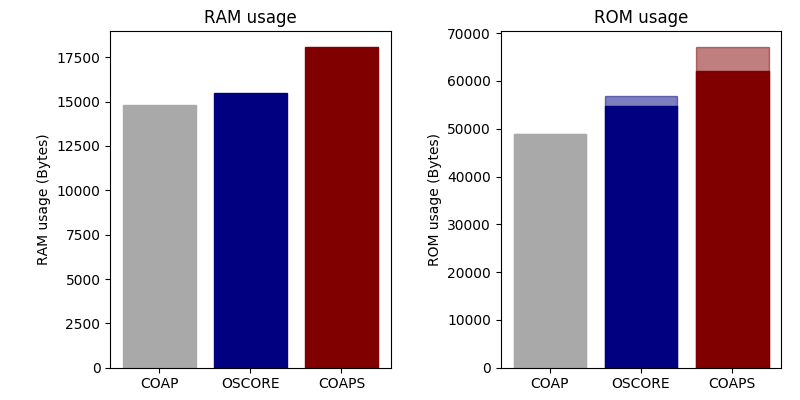
\includegraphics[width=0.8\textwidth]{papers/oscore/images/memory.png}
\caption[Memory utilization]{Memory utilization. The lighter parts in the ROM usage graph on the right indicates the memory used for the DTLS Handshake (in the "COAPS" test case) and for cryptographic primitives (in the "COAPS" and "OSCORE" test cases).}
\label{fig:memory}
\end{figure}

We can see that OSCORE uses less RAM and ROM than DTLS. Furthermore, OSCORE only uses $2\%$ more RAM than COAP, while COAPS uses $17\%$ more RAM than COAP. When comparing the ROM usage excluding cryptographic primitives, OSCORE uses $12\%$ more ROM than COAP, while COAPS uses $27\%$ more ROM than COAP when excluding the DTLS Handshake protocol and cryptographic primitives.

\subsection{Radio usage}
Figure \ref{fig:energest} shows the radio utilization rates for the tested protocols. The left graph shows the percentage of time spent in transmit mode while the right graph shows the percentage of time spent in listening mode. 

\begin{figure}[ht]
\centering
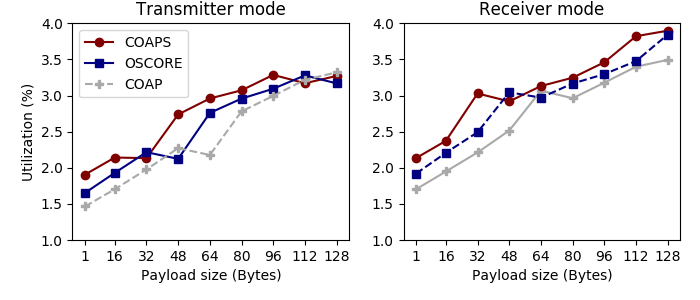
\includegraphics[width=0.9\textwidth]{papers/oscore/images/energest-radio.png}
\caption[Radio measurements]{Measurements of radio time occupancy for transmit and receive for the three protocols.}
\label{fig:energest}
\end{figure}

Compared to COAPS, OSCORE displays less radio usage when transmitting messages for most packet sizes. The time in listening mode is also smaller for OSCORE for most payload sizes. We conclude that OSCORE requires less network resources compared to COAPS.

These results were acquired using Energest, which uses timers to measure the time the radio has spent in either transmit-mode or receive-mode. Note that switching one timer off and the other on, e.g. going from transmit-mode to receive-mode cannot be done instantly. Therefore, the sum of the time in transmit-mode and the time in receive-mode does not always add up to the total elapsed time. However, the difference between these times and the error percentage is negligible.

\subsection{Energy usage}
We used Energest to measure the energy used for CPU, radio transmission and radio receiving by the different protocols for a message transaction. These results, along with a summation of total energy usage, can be seen in Figure \ref{fig:energy}.

\begin{figure}[ht]
\centering
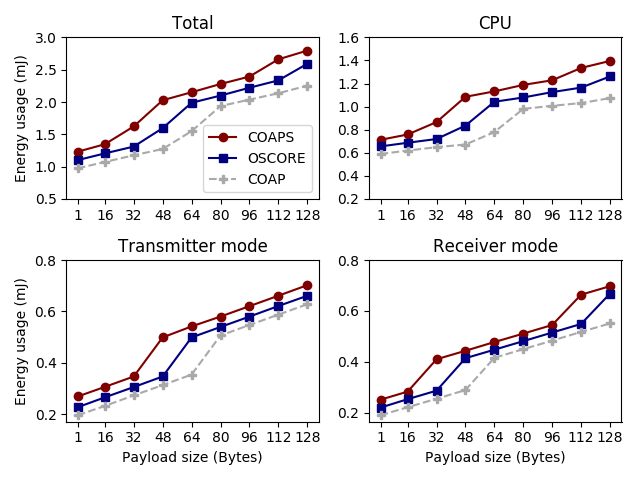
\includegraphics[width=0.8\textwidth]{papers/oscore/images/energest-energy.png}
\caption[Energy Consumption per exchange]{Energy consumption per message exchange. Note that scales are different for the y-axes.}
\label{fig:energy}
\end{figure}

We can see that the impact of the CPU power consumption is larger than the impact of the radio power consumption. A contributor to this is the fact that these CPU measurements include power consumed when the CPU idles in between messages (which are sent at a rate of 10 messages per second). This factor can be reduced by letting the CPU sleep instead of idling in between messages.

Most significant, we can see that OSCORE uses less energy in total compared to COAPS for all payload sizes. OSCORE has a per-exchange energy consumption about 8-28\% higher than COAP. This shows that OSCORE is more energy efficient than COAPS, which has an energy consumption about 17-59\% higher than COAP.

\section{Conclusion}
\label{sec:conclude}
We have presented OSCORE, a method for securing CoAP messages at the application layer based on object security. Unlike channel security approaches such as the DTLS protocol, OSCORE always ensures end-to-end security between client and server, even in the presence of intermediary (untrusted) proxies, with additional benefits in terms of privacy. OSCORE has been recently standardized as a security protocol at the Internet Engineering Task Force (IETF) \cite{cite:oscoap}. We have evaluated our implementation of OSCORE for the Contiki OS against DTLS on the SmartRF resource-constrained platform. Experimental results show that OSCORE outperforms DTLS in important metrics, namely radio transmission overhead, round trip time as experienced by CoAP clients, and memory usage as well as energy efficiency for constrained servers. Future work will focus on using OSCORE to secure multicast CoAP messages in use cases relying on group communication.

\section*{Acknowledgements}
The authors sincerely thank the anonymous referees and the associate editor for their insightful comments and suggestions. This work received funding from the European Union's Seventh Framework Programme for research, technological development and demonstration under grant agreement no. 607109. This work was also supported by the EIT-Digital High Impact Initiative ACTIVE; VINNOVA for the Celtic-Plus project CyberWI and the Celtic-Next project CRITISEC; SSF Grant RIT17-0032 and the Wallenberg AI, Autonomous Systems and Software Program (WASP) funded by the Knut and Alice Wallenberg Foundation. The authors thank Rikard H\"{o}glund and Jiye Park for their help and comments.


{\raggedright
        \printbibliography[segment=\therefsegment,heading=subbibliography]
}


\fi

\ifpaperIV
\newrefsegment
\addtolength{\apa}{2cm}
\fancyhead[RE]{\truncate{.95\headwidth}{\paperref{ch:digital-twin}: \paperIVtitle}}
\chapter[\paperIVtitle]{\texorpdfstring{%
                \paperIVtitle}{%
                \paperIVtitle}}

\label{ch:digital-twin}
\paperRemark{This is the full version of the paper below.
        This version contains an extended background description, and a more detailed motivation behind choices in the implementation as well as evaluation.

        \paperIVref}


%\theoremstyle{definition}
%\newtheorem{definition}{Definition}[section]


\section{abstract}
The digital twin is a rather new industrial control and automation systems concept. While the approach so far has gained interest mainly due to capabilities to make advanced simulations and optimizations, recently the possibilities for enhanced security have got attention within the research community. In this paper, we discuss how a digital twin replication model and corresponding security architecture can be used to allow data sharing and control of security-critical processes. We identify design-driving security requirements for digital twin based data sharing and control. We show that the proposed state synchronization design meets the expected digital twin synchronization requirements and give a high level design and evaluation of other security components of the architecture. We also make performance evaluations of a proof of concept for protected software upgrade using the proposed digital twin design. Our new security framework provides a foundation for future research work in this promising new area.

\section{Introduction}
\label{sec:digital-twin:introduction}

Industrial Automation and Control Systems (IACS) is a very broad term covering everything relating to control, monitoring and production in different industries and encompasses all parts of such systems.

While security for IACS in the past was neglected, in recent years security has obtained a lot of attention in the research community and indeed within the industry. Major security incidents such as the STUXNET worm in 2010 \cite{Falliere2011}, the Shamoon Saudi Aramao spear-phishing attack in 2012 \cite{Leyden2012} and the German steel factory attack in 2014 \cite{Roberts2014} have highlighted the risk of attacks on IACS.  Even if the attacks have been of many different types and origins, they have highlighted the need for enhanced security mechanisms and countermeasures. 

Clear evidence that the industry nowadays takes security issues seriously is the development of best practice security guidelines \cite{Didier2014} and the large number of security standards targeting the IACS domain, like ISO/IEC 27000 series\footnote{https://www.iso.org/isoiec-27001-information-security.html}, the ISA/IEC IEC 62443 series\footnote{ISA, ISA99, Industrial Automation and Control Systems Security, https://www.isa.org/isa99/} and the NIST SP800 series. Among those, IEC 62443 is based on the very general ISO 27000 but specified for the IACS area and also the NIST SP 800-82 \cite{NISTICS2015} in the SP800 series is an IACS standard. In addition, the industrial internet consortium has developed a new security framework \cite{Schrecker2016}. 

New technology trends affect IACS as well as the entire society. Security solutions, security recommendations as well as standards, need to adapt to the new technologies. One clear current trend is the move from legacy ISA-95 to highly distributed and cloud based architectures according to the Industry 4.0 and RAMI 4.0 models \cite{Lee2014}. This transition is demanding in many  ways, one challenge is control and information sharing between production units and cloud based control functions. This constitutes a major security risk and requires careful system engineering not to jeopardize IACS reliability \cite{Delsing2017}. We tackle this general security issue in this paper by looking into the digital twin model as an {\it enabler} for enhanced security when opening up IACS low level control functions and data exchange according to the Industry 4.0 vision. Digital twins and state replication as security enablers were recently proposed by different researchers \cite{Bittion2018},\cite{Eckhart2018}, \cite{Eckhart2018_2}. Previous works have not taken an IACS holistic view and in this paper we look into the problem from a system security point of view. The work is focused on identifying main design driving requirements for a digital twin based IACS security architecture and with special attention to a state synchronization model fulfilling the requirements. Detailed design of the different components and protocols in the architecture as well as formal security analysis of these are left for future work. 
The main contributions of the paper are the following:
\begin{itemize}
    \item We introduce a digital twin IACS adversary model and identify security requirements for this model.
    \item We suggest a novel digital twin based security architecture including a new state replication model.
    \item We evaluate the security of the proposed state replication model as well as present a proof of concept implementation  for a PLC software upgrade case including performance figures.
\end{itemize}
We proceed as follows: we discuss the digital twin model and make basic definitions which we use throughout the paper (\S \ref{Dtwinconcept}), we introduce our adversary model and derive security requirements (\S \ref{dtwinsecurity}),  we suggest a new digital twin security architecture and a novel digital twin design, including a state replication model (\S \ref{architecturedesign}). We make a security analysis of the proposed model and architecture (\S \ref{analysis}) and present a proof of concept implementation, including performance figures (\S \ref{analysis:manufacturing_example}). Lastly we discuss related work (\S \ref{sec:digital-twin:relatedwork}) and conclude (\S \ref{sec:digital-twin:conclusion}).

\section{Digital twin concept, related work and definitions}
\label{Dtwinconcept}
\subsection{Digital twin model and scenario}
\label{Dtwinconcept:model}
The digital twin was according to Grives \cite{Grives2014}, a terminology invented around 15 years ago by John Vickers of NASA and the term was introduced publicly by NASA in 2010 \cite{Shafto2010}. Originally, the concept was used to refer to the digital representation of a product used in simulations software but has been expanded to a concept where not only a physical product is represented in virtual form (software) but each product is directly connected with a virtual counterpart, the digital twin. The general model is depicted in Fig. \ref{figure:digital_twin_model}.

\begin{figure}[ht]
   \centering
    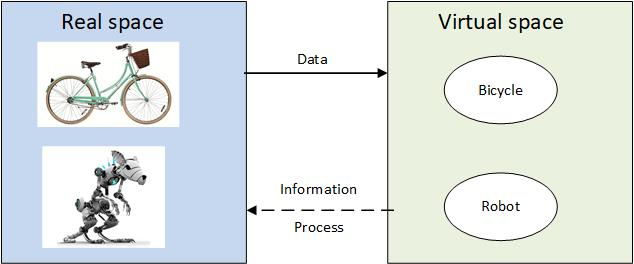
\includegraphics[scale=0.5]{papers/digital-twin/images/FIG1_TII-19-1326}
    \caption{The original digital twin model.}
    \label{figure:digital_twin_model}
\end{figure}

The overall goal with this concept is to be able to closely follow products during production (the physical twin) and simulate the process to adjust the production with results of these simulations. This can be done in real-time or close to real-time to optimize production flows etc. \cite{UHLEMANN2017}. The concept has then been extended to include all units (robot loading stations, conveyor belts etc.) in a production system allowing advanced simulations of a complete manufacturing system and the units involved in an autonomous system \cite{ROSEN2015}. Typically, then the digital twin part is represented and executed on cloud resources \cite{Shahriar2018}. Fig. \ref{figure:digital_twin_cloud} illustrates the overall scenario and model. 

\begin{figure}[ht]
   \centering
    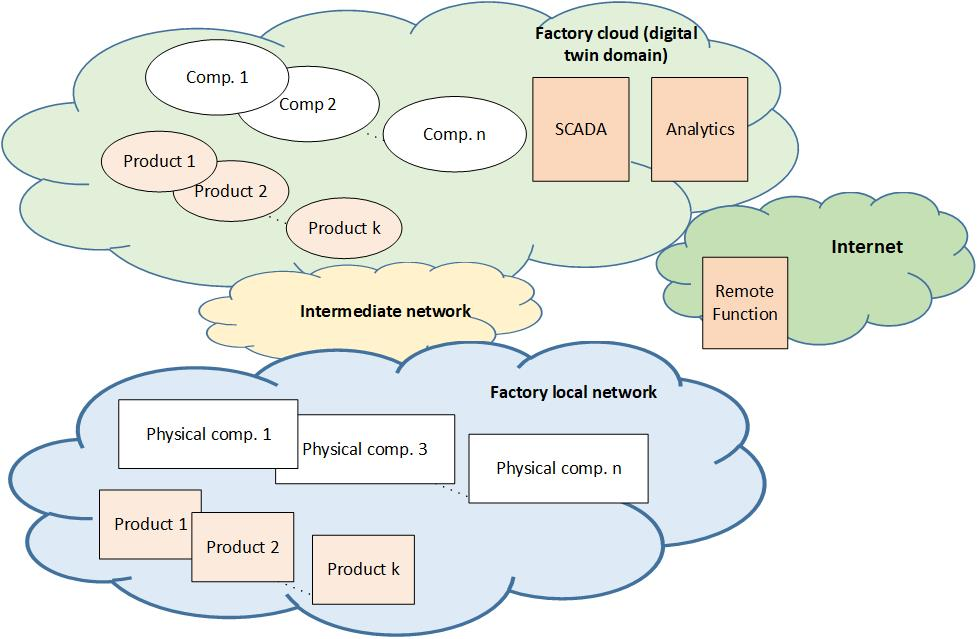
\includegraphics[scale=0.34]{papers/digital-twin/images/FIG2_TII-19-1326}
    \caption{Digital twin cloud system scenario.}
    \label{figure:digital_twin_cloud}
\end{figure}

As can be seen in Fig. \ref{figure:digital_twin_cloud}, according to this model not only are the products themselves reflected as digital twins in the virtual (cloud) domain but also the manufacturing units or what we here refer to as "components". Typical components here are PLCs, historians, sensors, actuators data acquisition units, HMI units etc. Several different models and principles for reflecting such units are possible \cite{Eckhart2018_2}. Here we focus on the network and logical state of a physical twin rather than the physical properties. The definitions and notations we use are introduced in Section \ref{Dtwinconcept:notations} below.

\subsection{Related work}
\label{sec:digital-twin:relatedwork}
Lots of work has been devoted to security in IACS. We will here briefly discuss literature surveys and how our architecture relates to the main security issues previously identified. Next, we will discuss some important previously introduced digital twin models and their relations to our approach. We mainly focus on prior work devoted to digital twin and state replication as enablers for enhanced security. 

Security in IACS in general has been treated in several good surveys \cite{krotofilgollman2013, uchenaEtAl2017}. The work by Krotifil and Gollmann \cite{krotofilgollman2013} focusing on different types of attacks on existing systems but also concluding that most efforts so far have been devoted to IDS. Many existing IDS are compatible with our suggested architecture but it has the benefit that such systems can be deployed in the virtual domain. A very broad systematic overview of security in cyber-physical systems in general (including IACS) is given in by Humayed \emph{et al.} in \cite{HumayedEtAl2017}. The authors identify that major security challenges in IACS are change management (including SW update) as well as the ability to handle legacy systems. Both these issues are tackles with the architecture we proposed in this paper. In addition, as we discussed in the introduction, several existing standards and new standard initiatives, are addressing IACS security in current and future systems. None of the main standardization bodies have so far been working with the digital twin concept as an enabler for enhanced security.

State machine replication has a very long history. Most of the work in this domain has been devoted to \textit{fault tolerance} \cite{Lamport:1978, Schneider1990}. Achieving state replication under the assumption of fault is much more demanding than the security oriented state replication we consider in this paper. We use a different, simpler model, allowing to choose the correct level of state reflection on the digital twin side depending on the security needs (see our state replication model in Section \ref{Dtwinconcept:replication}).  This is justified by the fact that the design goal of a digital twin security system is disparate from a fault tolerance system, as the digital twin cannot replace the physical twin if it fails, but is there to reflect the physical twin and protect it from direct, potential hostile, external interactions.

The digital twin model was first introduced in \cite{Shafto2010}. Lots of work has then been devoted to the topic in resent years and good overview is given in \cite{Negri2017}. The main focus has been on support of health analysis and improved maintenance as well as digitally mirroring the life of the physical entity. We are following the second approach but different from prior the majority of prior art, we are focusing on using the digital twin as an enabler for enhanced security.  

The usage of digital twins for penetrations testing is discussed in a recent work by Bitton \emph{et al.} \cite{Bittion2018}. The author investigate the relation behind a penetration test specification and system realization with focus on system cost optimization. A non-linear programming solution to find an optimal digital twin implementation level needed to perform  certain security analysis tasks is presented. This is an approach that also is applicable to the sub-problem of digital twin realization in a system realizing the security architecture we present in this paper. 

In \cite{Gehrmann2016} the idea of using state synchronization as an IoT security enabler was suggested. However, the model presented in \cite{Gehrmann2016} does not cover state changes on the IoT device side and no complete digital twin state synchronization model is given. Most recently, a digital twin security framework was presented in \cite{Eckhart2018_2} and later extended in \cite{Eckhart2018}. In \cite{Eckhart2018_2}, a digital twin specification principle using Automation ML (AML)\footnote{Actually, automation ML for digital twin modelling was already suggested by Grecyce  \emph{et al.} in 2016 \cite{Greyce2016} but not for any security applications.} was described together with a proof of concept implementation detecting a man-in-the-middle PLC attack. In the follow up work, \cite{Eckhart2018}, also the state replication problem is considered. In this work, a passive state replication model is presented where state updates are purely done based on inputs in the physical domain. The strength with such a model is that it avoids the negative performance impacts of active state monitoring. Inspired by the work in \cite{Eckhart2018_2} and \cite{Eckhart2018}, we have also looked into the problem area of state modeling as security enabler. However, different from the work in \cite{Eckhart2018}, we are looking into how digital twin can protect IACS from {\it external} attacks and not attacks on the factory domain. With this goal, we have proposed a different state propagation model and a security design allowing to  identify attacks at the virtual domain and preventing them for even reaching the physical domain. Furthermore, we have analyzed a complete digital twin system scenario and proposed an overall security architecture for such scenario.

\subsection{Digital twin definition and notations}
\label{Dtwinconcept:notations}
For the purpose of the paper we denote by $u \in U$, a physical twin, where $U$ denotes the set of physical twins in the system. Similarly, we denote by $u' \in U'$, a digital twin where $U'$ is the set of digital twins in the system.  Let then $S_u = \{s_{u0},s_{u1},...,s_{um-1}\}$ and $S_{u'} = \{s_{u'0},s_{u'1},...,s_{u'n-1}\}, m \geq n$, be the finite set of states of $u$ and $u'$, i.e., we assumes that the digital twin always only reflects a {\it subset} of the physical twin states and no states which are not represented in the physical twin.  Furthermore, denote by $I_u = \{i_{u0},i_{u1},...,i_{ur-1}\}$ the set of possible finite inputs to physical twin $u$ and by $I_{u'} = \{i_{u'0},i_{u'1},...,i_{u'd-1}\}$, the set of finite possible inputs to digital twin $u'$. We denote by $s_{u,t}\in S_u$,  the state of physical twin $u$ at clock cycle $t$ and by $i_{u,t}\in I$ the input to $u$ at clock cycle $t$. Similarly, denote by $s_{u',t} \in S_{u'}$,  the state of digital twin $u'$ at clock cycle $t$ and the input to $u'$ at clock cycle $t$ by $i_{u',t} \in I'$. Hence, the initial state of the physical twin is $s_{u,0}$ and the initial state of the digital twin is $s_{u',0}$. Then we can define both the physical and digital twin as finite state machines. We then let $\delta_u: S_u \times I_u \rightarrow S_u$ and $\delta_{u'}: S_{u'} \times I_{u'} \rightarrow S_{u'}$ be the transition functions for the physical and digital twin respectively, i.e. $s_{u,t+1} = \delta_u(s_{u,t},i_{u,t})$ and $s_{u',t+1} = \delta_{u'}(s_{u',t},i_{u',t})$. 

We assume a clock based digital twin state synchronization model where a each clock cycle, $t$, the state of the twins are synchronized with a message exchange starting with a first synchronization message from the $u'$ to $u$ and with a response synchronization message from  $u$ to $u'$. We denote these message as $m_{u'\rightarrow u}(t)$ and  $m_{u \rightarrow u'}(t)$, respectively. These messages are typically not transferred in clear between the twin and intermediate nodes, but in protected/transformed form. We denote protected version of the synchronization messages by $e_{u'\rightarrow u}(t)$ and  $e_{u \rightarrow u'}(t)$.

\section{Adversary model and security requirements}
\label{dtwinsecurity}
Next, using the digital twin model and definition introduced in Section \ref{Dtwinconcept}, we describe a digital twin threat model. Using this threat model we identify security requirements for a digital twin based IACS architecture.
\vspace*{-0.15in}
\subsection{Adversary model}
\label{dtwinsecurity:adversary}
Adversary models for digital twin systems have not been extensively treated in the literature as the concept mostly so far has been used  for production optimization and not security. Certain security aspects regarding using digital twin as security enablers in IACS are considered in \cite{Eckhart2018}  and \cite{Bittion2018}. The authors in \cite{Eckhart2018} consider state replication for active monitoring and intrusion detection while \cite{Bittion2018} consider the problem of penentration testing of IACS with focus on cost optimization for specific security penetration tests (performed on simulated or emulated digital twin or on an acutal physical component in the IACS). However, since these works have very specific security functions goals, they lack adversary model definitions for the digital twin scenario we are considering. Hence, we have developed a new adversary model below. This is {\it not} a generic digital twin adversary model but a model that makes sense in systems with cloud based data sharing and control in IACS. We also give the main motivations for using this rather restrictive adversary model. 

Traditionally, IACS has been separated with firewalls from other networks such as corporate network and the internet.  Several good architectures and recommendations are available  \cite{Schrecker2016}. Here, we assume such principles are deployed and we have adopted an adversary model where we \textit{do not} consider any attacks on the physical twin part or local factory network part of the system but assume these parts can be properly isolated from hostile external networks\footnote{Internal factory network attacks are of course also possible, but we do not consider those in our adversary model.}. 

We assume that the digital twin can run in a separate process even on a third party cloud resource. Then the digital twin can be realized using virtualization techniques where the virtualization is offered on the most suitable level \cite{Smith2005}. Providing strong isolation for virtualization and protection against hostile cloud providers is a very challenging topic which has been widely addressed with several different models and solutions the past ten years \cite{Liu2015, Schuster2015, Paladi2017}. Recent attacks Metldown \cite{Lipp2018} and Spectre \cite{Kocher2019} have shown that one cannot even trust the fundamental hardware functions needed for secure isolation currently in use. However, the security with respect to secure execution environment for virtualized systems is steadily improving and we will for simplicity in this paper disregard attacks on the isolation properties of the digital twin and assume that a secure execution environment and data storage is provided for the digital twin in the system.

We adopt the Dolev-Yao model \cite{Dolev1981} and assume that the attacker can influence the system in all other aspects including the following capabilities of the adversary:
\begin{itemize}
    \item The attacker is able to intercept, modify and replay all communication from the physical domain to the digital domain and vice versa.
    \item The attacker is able to launch input attacks by sending arbitrary messages to a digital twin and input requests, i.e. he or she can choose to send arbitrary input from the set $I_{u'}$ to the digital twin $u'$.
    \item The attacker is able to launch intercept, modify and replay any information sent between digital twins or between digital twins and other units executing in the virtual domain.
\end{itemize}

\subsection{Security definitions}
Next, we give basic security definitions. The basis of the new security architecture is the introduction of state replication between the physical and digital twin. An expectation from such model from \emph{robustness} perspective is that the synchronization is accurate over all system states and inputs. The synchronization consistent expectation is fundamental for deploying the architecture and very different from architectures introduced in the literature before. The main reason why consistency is important is that without it, one cannot rely on that all system changes in the digital twin part are correctly propagated to physical part of the system and vice versa, which will make it impossible to use the model in practise as the system behaviour would be unreliable. Hence, even if the synchronization consistency not is a pure security requirement, it is fundamental for the proposed architecture and we make a precise definition of synchronization consistent ency. It is also important to notice that one would expect from a specific design and implementation of our architecture to provide the synchronisation consistency property also under attack conditions. Hence, it is important to introduce a proper definition also in this regard.

Another fundamental, pure security expectation, with respect to the synchronization is the confidentiality and integrity of the synchronization process as such. Hence, we also provide precise definitions for these two aspects.  Apart from these definitions, we adopt widely used computer and communication security definitions \cite{Stallings2014}.

\label{dtwinsecurity:defintions}
\theoremstyle{definition}
\begin{definition}
\label{dtwinsecurity:consistent}
A digital twin system is \emph{consistent} if there exist functions $\forall u \in U,f_u: S_u\rightarrow S_{u'}$such that the following is true:
\begin{eqnarray}
    \forall s \in S_u, f_u(\delta_u (s,\emptyset))  & =  &\delta_{u'}(f_u(s),\emptyset),\label{dtwinsecurity:const1}\\
	s_{u',0} & = &f_u(s_{u,0}). \label{dtwinsecurity:const2}
\end{eqnarray}
\end{definition}

This definition reflects the requirement that when the digital twin starts in a state consistent with the staring state of the physical counterpart and whenever neither the physical twin nor the digital twin receive any input, they are both always transitioned to states that are consistent. i.e. the physical to digital twin state mapping agree with the state of the digital twin.

\begin{definition}
\label{dtwinsecurity:confidentiality}
A digital twin system synchronization protocol provides \emph{confidentiality protection} if an adversary, who observes information, $e_{u'\rightarrow u}(t)$ and $e_{u\rightarrow u'}(t))$, sent from the digital twin and from the physical twin respectively at time $t$,  cannot execute any attack, $A$, that in polynomial time will allow the attacker to distinguish the state of the physical twin from any randomly selected state, i.e., after execution of $A$, the following is true: 
\begin{eqnarray}
    \forall s \in S_u,  Pr(s_u = s|e_{u'\rightarrow u}(t), e_{u\rightarrow u'}(t)) = Pr(s_u = s) \label{dtwinsecurity:eqconfidentiality}
\end{eqnarray}
\end{definition}

\begin{definition}
\label{dtwinsecurity:synchprot}
A digital twin system synchronization protocol provides \emph{synchronization protection} if the adversary cannot execute any attack replacing message exchange $e_{u'\rightarrow u}(t)$ with $e'_{u'\rightarrow u'}(t)$ and/or replacing $e_{u\rightarrow u'}(t)£$ with $e'_{u\rightarrow u'}(t)$ which will be accepted by $u$ and $u'$ and making the twins out of synchronization, i.e.  $f_u(s_{u,t}) = s_{u',t}$ is always true after successful synchronization independent of adversary substitution choices\footnote{This definition does {\it not} take a DoS attack into account and assumes that the synchronization messages arrives at each time slot.}.
\end{definition}

\begin{figure}[th]
\hspace*{-0.2in}
   \centering
    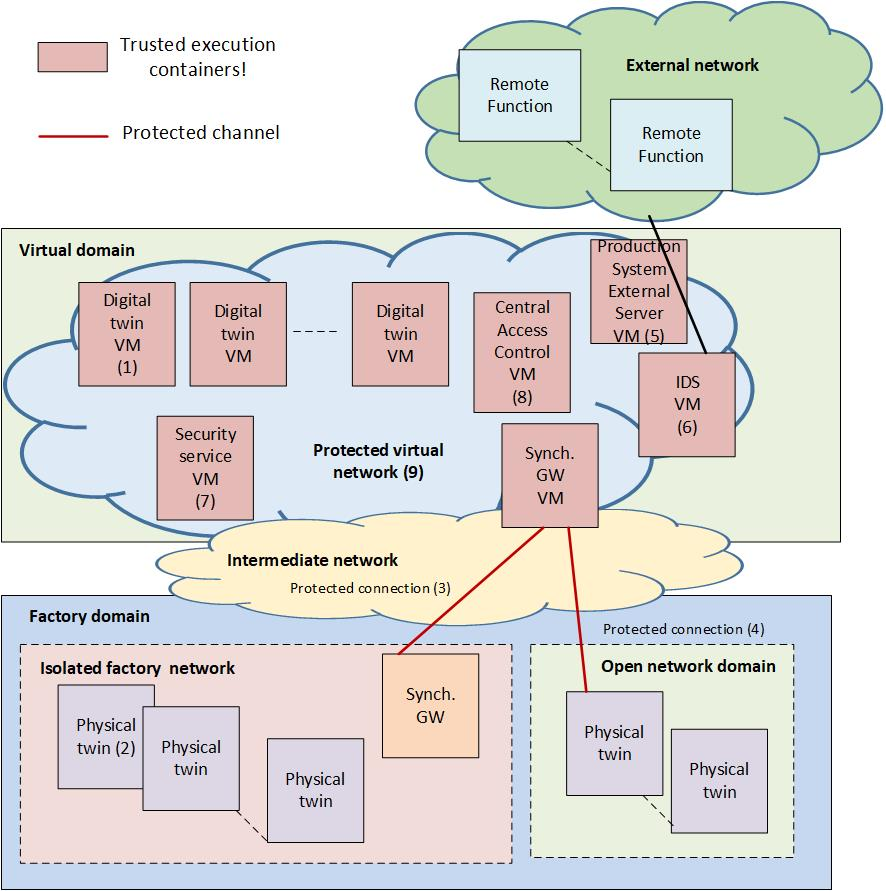
\includegraphics[scale=0.35]{papers/digital-twin/images/FIG3_TII_191326}
    \caption{Security architecture overview.}
    \label{figure:security_architecture}
    
\end{figure}
\vspace*{-0.2in}
\subsection{Requirements}
\label{dtwinsecurity:requirements}
We have used the previously presented adversary model and security definitions to identify a set of system security, performance and accuracy requirements. This is not an exhaustive list but the major identified system architecture requirements.
\begin{labeling}{R6.}
\item [R1.] \textbf{Synchronization security:} We require the digital twin state replication model and protocol to be consistent (Definition \ref{dtwinsecurity:consistent}), provide confidentiality protection (Definition \ref{dtwinsecurity:confidentiality}) and synchronization protection (Definition \ref{dtwinsecurity:synchprot}).
\item[R2.] \textbf{Synchronization latency:} The synchronization message exchange must not cause any delays which prevent time critical control functions to be propagated to from the physical to the digital twin. The precis requirements are application dependent.
\item[R3.] \textbf{Digital twin external connections protection:} All connections between the digital twin and the external entities must be authenticated. According to the adopted adversary model, we assume each digital twin to run in a protected execution environment but all request external to this environment must be properly authenticated and all information sent from the digital twin to external trusted parties must be confidentiality and integrity protected. 
\item[R4.] \textbf{Access control:} The digital twin itself or a secure entity in direct connection with the digital twin needs to make sure access control is applied on on all incoming requests.  This includes request and information exchange with external parties as well as information exchange with other digital twins. 
\item[R5.] \textbf{Software security:} The physical twin software must always be in a trustworthy state. This implies that the physical twin must be protected from installation of harmful software. Mechanisms shall be in place to recover the system in case of zero-days attacks on the physical twins.
\item[R6.]\textbf{Local factory network isolation:} The local factory network shall not accept any connection requests except for protected synchronization requests with the digital twin (see R1 above).  Physical twins should be protected from DoS attacks through boarder unit such as a gateway or firewall making sure that only protected synchronization requests reach a physical twin and no other outside traffic.
\item [R7.] \textbf{Digital twin Denial-of-Service (DoS) resilience:} The digital twin must be protected from DoS attacks such as network flooding or distributed DoS directly targeting a digital twin. Proper DoS filters and router configurations must be deployed in the factory cloud domain to prevent or limit the DoS possibilities of the attacker. At the same time, filters and router policies must not prevent synchronization exchanges to reach the digital twins in the system.
\end{labeling}

\section{A digital twin based security architecture and state replication design}
\label{architecturedesign}

\subsection{Security architecture}
\label{dtwinsecurity:architecture}
We now have the definitions and requirements in place to define a generic digital twin security architecture. Fig. \ref{figure:security_architecture} gives a high-level picture of the proposed architecture. We have here focused on the main security properties and entities in the system. This is {\it not} a complete design in all details but a high level design including main components and their roles in the architecture. We verify the key digital twin design of it in our proof of concept evaluation but leave detailed design and evaluation of other components for future work.

A basic security assumption in this architecture is the possibility to launch digital twins as well as security services in \textit{trusted execution containers} as Virtual Machines (VMs) on suitable cloud resources. The architecture is completely agnostic on the virutalization technique used for this or on which actual level the vitalization is applied  \cite{Smith2005} \cite{Gehrmann2016}. However, the architecture requires the virtualization technology to provide trusted execution in the sense that different VMs are strongly isolated from each other and that they have access to protected volatile and non-volatile storage.

Using the numbering introduced in Fig. \ref{figure:security_architecture}, we discuss the different properties of the components in the architecture below.
\subsubsection{Digital twin component} The digital twin component is running as a VM in an isolated environment. An overview picture of the main logical functions of the twin is given in Fig. \ref{figure:dtwin_security_architecture}. The core functionality of the digital twin is the actual simulation of the physical counterpart. Only two direct external network interactions are allowed: the synchronization (which occurs over the synchronization GW) and the exchange with external requests and responses. This takes place either through the cloud server which takes \textit{all} incoming requests and responses from external entities or directly to other digital twins or back-end components. The virtual domain external connections are protected through the cloud Virtual Private Network (VPN) (see Section \ref{dtwinsecurity_secarch_VPN}). The state of the digital twin is \textit{exported} directly to a \textit{common} (for several digital twins in a system) security analysis component (see also Subsection \ref{dtwinsecurity:security_analysis}). Also the intermediate state, $\hat{s}_{u'}$, is exposed to an analyzer in this way. This implies that an external analyzer can have access (if allowed by the access policy) to all digital twin states in the system. This in turn allows \textit{abortion} of state propagation in case of detection of a fatal security issue by the external analyzer. The digital twin has access to a secure clock, $t$, for precise synchronization operations with the physical twin.  The actual state propagation design we use is described in Section \ref{Dtwinconcept:replication}.

\begin{figure}[ht]
   \centering
    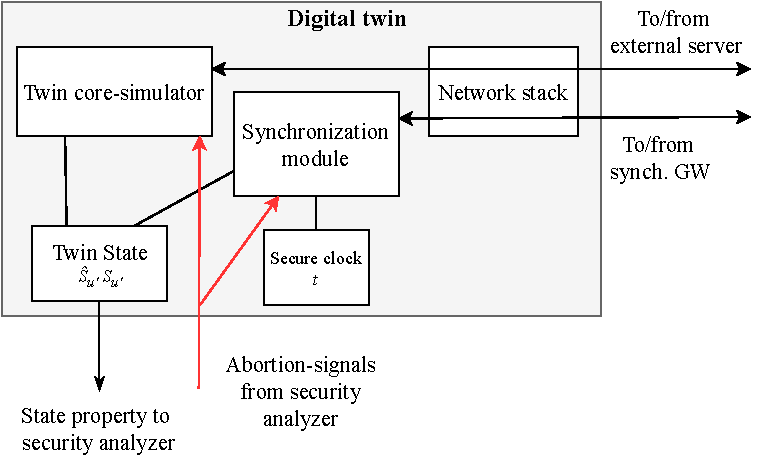
\includegraphics[scale=0.65]{papers/digital-twin/images/FIG4_TII-19-1326}
    \caption{Digital twin main functions}
    \label{figure:dtwin_security_architecture}
\end{figure}

\subsubsection{Physical twin component}
An overview picture of the main logical functions of the physical twin is given in Fig. \ref{figure:phytwin_security_architecture}. Similar to the digital counterpart, the physical twin executes the defined synchronization protocol. Depending on if the physical twin actually has network connectivity or not, it might run the synchronization itself or it is done through a ''measurement unit''\footnote{For a physical twin that is in production, it could be that it has no program execution capabilities, but its state is only measured through external sensors for instance.}. A physical twin deployed in an isolated factory network will only exchange synchronization information with a dedicated synchronization GW on the same network. On the other hand, a single deployed physical twin outside such a network will need to directly exchange synchronization information with the synchronization GW in the virtual domain and needs access to the key material needed for such secure interactions. The physical twin will apart from this, not need any specific security adaptations at all. The state propagation design applicable to the physical twin is described in Section \ref{Dtwinconcept:replication}.

\begin{figure}[ht]
   \centering
    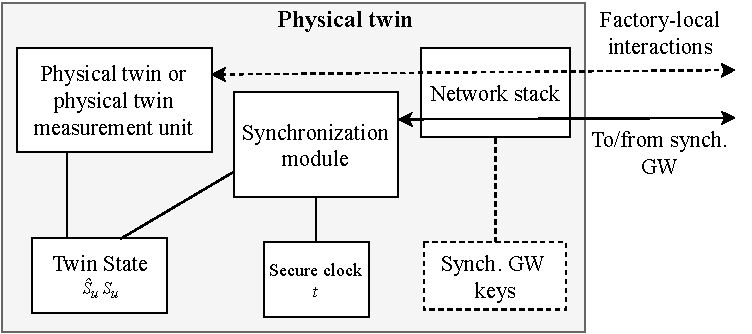
\includegraphics[scale=0.65]{papers/digital-twin/images/FIG5_TII-19-1326}
    \caption{Physical twin main functions.}
    \label{figure:phytwin_security_architecture}
\end{figure}

\subsubsection{Protected connection between synchronization gateways} 
\label{dtwinsecurity:arch_protected_connection}
The connection between the synchronization GW on the local factory and the virtual domain is protected through a secure channel. We have chosen this principle instead of end-to end synchronization protection as we assume it will be possible to deploy synchronization GWs in trusted containers in the virtual domain. Standard IPsec \cite{Kent2005} VPN or a TLS/DTL channels \cite{Dierks2008} \cite{rfc6347} are assumed. A major advantage with such solution from security management point of view is that this allows a \emph{single} security relation between the physical and digital domain. Such single relation is very easy to maintain from security perspective. For instance, can a pres-shared key TLS or DTLS relation for instance be used. This can be compared to a situation where external entities are allowed to directly connect to the physical domain. In such situation, each external connection would need a separate security relation with the physical domain. Now, such relations are instead moved to the digital domain, where the security risk is much lower and where it is much less complex to handle such relations from a security configuration management point of view.
\subsubsection{Protected connection from isolated physical twin to synchronization gateway}
A physical twin not deployed in a protected local factory network, needs to directly connect to the synchronization GW in the virtual domain. This connection then obviously needs to be confidentiality and integrity protected using a suitable secure channel (see Section \ref{dtwinsecurity:arch_protected_connection}).
\subsubsection{Production system external server}
The architecture assumes all external requests arrives in the virtual domain, i.e. external input to digital twin $u'$ from the set $I_{u'}$ arrives to the production system external server prior to (potential) being forwarded to the digital twin $u'$. Similar responses from a digital twin are routed through this sever as well. This allows advanced network filtering at a single point and avoids having such functionality duplicated at each digital twin virtual instance\footnote{Recall that in our adversary model we assume all inputs to a \textit{physical} twin to be trustworthy and not subject to direct security analysis}.
\subsubsection{Intrusion Detection System (IDS)}
State-of-the art IDS are best deployed at the boarder to the internet \cite{Kruegel2002}. We adopt this principle and assume the actual intrusion analysis to be done by a VM with direct access to the external network interface traffic. 
\subsubsection{Security analysis service} \label{dtwinsecurity:security_analysis}
The core benefit from a security perspective with a digital twin model like the one we have defined, is the possibility to do security analysis directly on the digital twin state and even on the states of a whole family of digital twins. By letting the analyzing engine having access not only to the final states, but also intermediate states, i.e. the $\hat{s}_{u'}$ states in the system, it is possible for a security analysis function to detect harmful state transitions (prior to the state propagating to the physical twin) and take direct action in the digital domain (see also Fig. \ref{figure:dtwin_security_architecture}).
\subsubsection{Central access control}
By letting all external digital twin access be subject to a single point access control, system wide policies can easily be deployed in the system.  Advanced security policies can be defined through standard access control frameworks such as Extensible Access Control Markup Language (XACML) \cite{Rissanen2013}. In order to allow direct interaction between digital twins, this is preferably combined with component local policy enforcement through tokens issued at the central access control entity using standard tokens such as SAML \cite{Campbell2015} or OAuth \cite{Hardt2012}. 
\subsubsection{Protected virtual network}
\label{dtwinsecurity_secarch_VPN}
Most cloud providers offer network isolation between VMs launched on cloud resources\footnote{https://docs.aws.amazon.com/vpc/index.html\#lang/en\_us}\footnote{https://docs.microsoft.com/en-us/azure/virtual-network/virtual-networks-overview}. Even if we have not assumed all trusted execution services to be deployed as complete, "traditional" VMs in the virtual domain, higher layer VMs can be launched on such VMs allowing re-use of standard principles for network isolation. There are also other, non-provider dependent solutions to achieve this \cite{Li2010}.

\subsection{State replication model and design}
\label{Dtwinconcept:replication}

Several different state replication principles for digital twins are possible. Recently, a specification-based state replication model for digital twins was proposed \cite{Eckhart2018}. We have adopted a similar physical and digital twin state transition model. However, the state replication design in \cite{Eckhart2018} is built upon measurement of input values and that the physical and digital twin runs {\it functional identical programs} or what the authors refers to as ''passive state replication''. This is an approach that is efficient if the main purpose of the design is to evaluate security breaches stemming from the physical domain. Instead, we in our security architecture use the digital twin as a ''guard'' against all, potential hostile, {\it external} stimuli on the physical domain. Hence, even if demanding from real-time perspective, we instead have adopted a direct state replication or what the authors in \cite{Eckhart2018} refers to as ''active monitoring''. This different security goal and approach also allow us to abandon the functional identical program requirements. 
We assume a model, where the physical and digital twin are synchronized on regular basis. Without loss of generality, we assume that a synchronization is done at each clock cycle. Let $z_u:S_u \times S_{u'}\rightarrow S_u$ be a synchronization function and $h_u: S_u \rightarrow S_{u'}$ a physical to digital state mapping function for twin $u$. The complete synchronization (including the twins state updates) then consists of the following operations:
\vspace*{-0.08in}
\begin{eqnarray}
\hat{s}_{u,t+1} & = & \delta_u(s_{u,t},i_{u,t}) \label{physprelsynch}, \\
\hat{s}_{u',t+1} &=& \delta_{u'}(s_{u',t},i_{u',t}) \label{digprelsynch}, \\
	s_{u,t+1} & = & z_u(\hat{s}_{u,t+1},\hat{s}_{u',t+1}) \label{digtsynch}, \\ 
	s_{u',t+1} & = & h_u(s_{u,t+1}). \label{physdsynch}
\end{eqnarray}
This synchronization model works such that the physical and digital twin treat their respective inputs independently. We assume that the input will change the state of the (respective) twins independently, and then at the next time slot, they will synchronize their states to make them consistent considering the inputs received before last synchronization. 

The choice of the functions $z_u$ and $h_u$ will depend on the digital twin model and the exact relation between the physical and digital twin. Many different models are possible. For the purpose of this paper, we choose a simple twin model but still a model allow to cover several important security cases as we show in Section \ref{analysis:manufacturing_example}. Denote by  $S_u = S1_u \bigcup S2_u \bigcup S3_u$, we then make the following assumption:  $S1_u \bigcap S2_u = S1_u \bigcap S3_u = S2_u \bigcap S3_u = \emptyset$. Let $S_{u'} = S1_{u'} \bigcup S2_{u'}$ and we assume that $S1_{u'} \bigcap S2_{u'} = \emptyset$. Then we can write the state of the physical twin as $s_u = (s1_u,s2_u,s3_u)$ and the state of the digital twin as $s_{u'} = (s1_{u'},s2_{u'})$. We then apply the following restrictions:
\begin{eqnarray}
 S2_u   & = &  S1_{u'}, \label{arch:s2eq}\\
 S3_u   & = & S2_{u'} \label{arch:s3eq}, 
 \end{eqnarray}
 \begin{eqnarray} 
 \forall s_u \in S_u,  \forall i_u \in I_u, \delta_u(s_u,i_u)   =  \nonumber \\  
 = (\delta1_u(s_u,i_u), \delta2_u((s2_u,s3_u),i_u), s3_u), \label{arch:phystransrestric}\\
  \forall s_{u'} \in S_{u'}, \forall i_{u'} \in I_{u'},  \delta_{u'}(s_{u'},i_{u'})   =  \nonumber \\  
 =   (s1_{u'}, \delta2_{u'}(s_{u'},i_{u'})) \label{arch:digtransrestric}
\end{eqnarray}

In addition, we let
\begin{eqnarray}
 s_{u',0}  =  (s1_{u',0},s2_{u',0}) = (s2_{u,0},s2_{u',0}), \label{arch:digsynchstart}\\
 s_{u,0}  =  (s1_{u,0},s2_{u,0},s3_{u,0}) = (s1_{u,0},s2_{u,0},s2_{u',0}) \label{arch:physsynchstart}
\end{eqnarray}

With these restrictions, we then let $z_u(\hat{s}_{u,t},\hat{s}_{u',t}) = (\hat{s}1_{u,t}, \hat{s}2_{u,t}, \hat{s}2_{u',t})$ and
\begin{equation}
h_u(s_{u,t+1})
= \left \{ \begin{array}{ll}
(s2_{u,0},s3_{u,0})   & \mbox{if $t<0$} \\
(\hat{s}2_{u,t+1}, \hat{s}2_{u',t+1}) & \mbox{otherwise}  \end{array} \right.
 \label{arch:zerostate}
\end{equation}

To send the \textit{complete} state at each synchronization occasion is very inefficient. Instead, the state changes (deltas) are calculated:
\begin{eqnarray}
m_{u'\rightarrow u}(t) & = & \Delta_{\hat{s}_{u'}} =  \textrm{Diff}(\hat{s}_{u',t+1},s_{u',t}), \label{arch:firstdelta} \\
m_{u \rightarrow u'}(t) & = & \Delta_{s_{u'}} = 
\textrm{Diff}(\hat{s}2_{u,t+1},s2_{u,t}), \label{arch:seconddelta}
\end{eqnarray}
This implies that the digital twin calculates a first delta, $\Delta_{\hat{s}_{u'}}$, and sends it to the physical twin. This delta is then used by the physical twin to reconstruct $\hat{s}_{u',t+1}$, which is the input to the $z$ function, i.e. equation (\ref{digtsynch}). Next, the physical twin calculates the ''return delta'', $\Delta_{s_{u'}}$ , that is sent back to the digital twin.   The principle is illustrated in Fig. \ref{figure:digital_twin_synch} below. Observe, that we here only illustrate the synchronization information exchange and not the protection of the synchronization messages as such. The protection principles we apply was described in Section \ref{dtwinsecurity:architecture}.

\begin{figure}[ht]
   \centering
    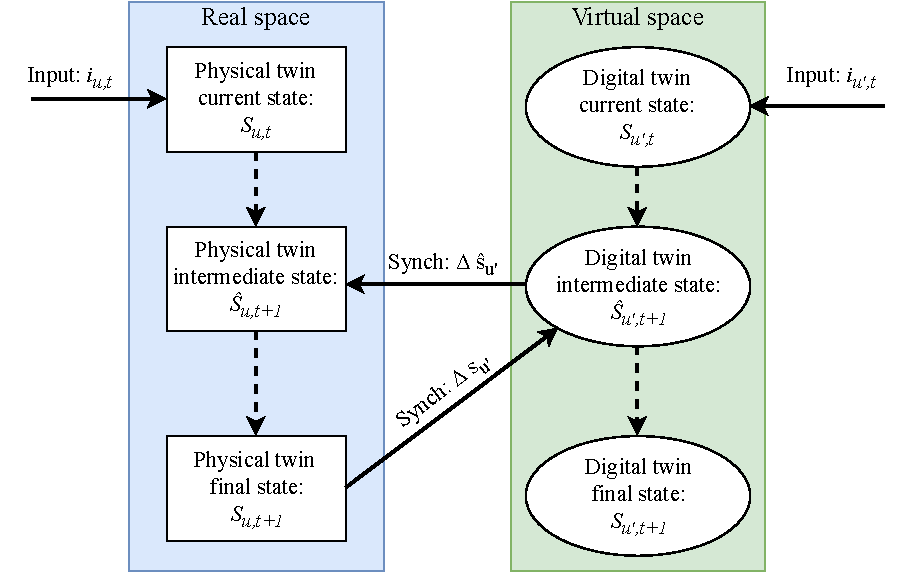
\includegraphics[scale=0.55]{papers/digital-twin/images/FIG6_TII-19-1326}
    \caption{Synchronization principle.}
    \label{figure:digital_twin_synch}
\end{figure}

It is important to notice from real-time and communication overhead perspectives that when no input is received neither on the physical or digital side, there is no need for the twins to exchange any deltas. This is true given a consistent digital twin system synchronized with accurate clocks.

\section{Security analysis}
\label{analysis}
Next, we analyze the proposed framework from security and performance perspectives. We here mainly focus on the synchronization security characteristics. We also give arguments regarding how the proposed architecture meets the other security requirements listed in Section \ref{dtwinsecurity:requirements}. As the architecture in many aspects only include a high level design, we here postpone detailed security evaluation of these aspects to future work and for specific implementation designs. 
\subsubsection{Synchronization security}
%\newtheorem{prop}{Proposition}
\begin{prop}
\label{analysis:synchsec}
The digital twin synchronization model and protocol is consistent.
\end{prop}
\begin{proof}
Let:
\begin{equation}
f_u(s) = f_u((s1,s2,s3)) = (s2,s3). \label{fdef}
\end{equation}
From (\ref{arch:physsynchstart}) we have that $s_{u,0} = (s1_{u,0},s2_{u,0},s2_{u',0})$ and from (\ref{arch:digsynchstart}) and (\ref{arch:zerostate}), it then follows that $f_u(s_{u,0}) = h_u(s_{u,0}) =  (s2_{u,0},s3_{u,0}) = (s1_{u',0},s2_{u',0}) = s_{u',0}$, which fulfils condition (\ref{dtwinsecurity:const2}).

Now, using the assumptions (\ref{arch:s2eq}),  (\ref{arch:s3eq}), (\ref{arch:phystransrestric}) and (\ref{arch:digtransrestric}), let: $\hat{\delta}_u(s_u,i_u) = (\delta1_u(s_u,i_u), \delta2_u((s2_u,s3_u),i_u), \delta2_{u'}((s2_u,s3_u),\emptyset)$. Then, it follows from (\ref{fdef}), $f_u(\hat{\delta}_u(s_u,\emptyset)) = (\delta2_u((s2_u,s3_u),\emptyset), \delta2_{u'}((s2_u,s3_u,\emptyset))$. Similar, let: $\hat{\delta}_{u'}(s_{u'},i_{u'}) = (\delta2_u((s1_{u'},s2_{u'}),\emptyset),\delta2_{u'}(s_{u'},i_{u'}))$. Then by direct calculation: $\hat{\delta}_{u'}(f_u(s_u),\emptyset) = \hat{\delta}_{u'}((s2_u,s3_u),\emptyset) = (\delta2_u((s2_u,s3_u),\emptyset),\delta2_{u'}((s2_u,s3_u),\emptyset)) = f_u(\hat{\delta}(s_u,\emptyset))$.
 By then letting the state $s_u$ taking any value in $S_u$, it follows that also condition (\ref{dtwinsecurity:const1}) is fulfilled.
\end{proof}
\begin{prop}
\label{analysis:proofconfidentiality}
If the secure channel used for communication towards and between synchronization GW in the architecture provides confidentiality, the digital twin synchronization design also provides confidentiality.
\end{prop}
\begin{proof}
According to our attacker model, an adversary can intercept any message sent from the digital twin to the synchronization GW in the virtual domain or any messages sent between synchronization GWs. He or she might also intercept message sent from physical twins towards the GW deployed in the virtual domain. The attacker has no other option to intercept any synchronization information.
According to (\ref{arch:firstdelta}) and (\ref{arch:seconddelta}), at each clock cycle, one delta message is sent from the digital twin towards the physical twin and a replay delta message is sent in return. An adversary has two options to intercept the first message, $e_{u'\rightarrow u}(t)$; Either he or she intercept it when it is sent from the digital twin the synchronization GW in the virtual domain {\it or}\ when it is forwarded from the synchronization to the GW in the factory domain (or physical twin in the second option). As long as both these channels provide confidentiality the attacker will not get any information on $s_u$. As the return message follows the very same path, the also the return message, $e_{u \rightarrow u'}(t)$ , will have the very same protection and equation (\ref{dtwinsecurity:eqconfidentiality}) is fulfilled.
\end{proof}
\begin{prop}
If the secure channel used for communication towards and between synchronization GW in the architecture provides integrity and replay protection, the digital twin synchronization design also provides synchronization protection.
\end{prop}
\begin{proof}
According to Proposition \ref{analysis:synchsec} the proposed synchronization model is consistent and consequently if no input is received on neither the digital nor physical twin, $h_u(s_{u,t+1}) = s_{u',t+1}$. Furthermore, if the synchronization messages also arrives unmodified equation (\ref{physdsynch}) guarantees that $h_u(s_{u,t+1}) = s_{u',t+1}$ holds also in this case. Hence, the only option for an attacker would be to modify any messages $e_{u'\rightarrow u}(t)$ or $e_{u\rightarrow u'}(t))$. In analogue with the proof of Proposition \ref{analysis:proofconfidentiality}, if the used secure channels provides integrity and replay protection, such modification will be detected and a modified or replayed message will be rejected.  
\end{proof}
\subsubsection{Latency}
The architecture as such does not make any direct assumption regarding the synchronization real-time behaviour. Depending on the specific IACS application, the networks must be chosen and configured accordingly. Similarly, the synchronization GW must be implemented on platforms powerful enough to fulfill real-time requirements. For some applications, deploying the virtual domain on an edge cloud \cite{Delsing2017} can be used to meet R2.  
\subsubsection{External connections}
The architecture assumes all external connection to be intermediates by the external server entity at the boarder of the external network. The external server will only accept authenticated requests. Furthermore, the final hop for the external server to the digital twin runs through the virtual domain VPN. This, if properly implemented, implies that the system fulfills the requirement R3. 
\subsubsection{Access control}
According to the proposed security architecture, the centralized access control VM deployed in the virtual domain makes sure all access requests towards the digital twin are properly authorized. Access control enforcement then takes place at the digital twin VM. This means that the main building blocks are included to fulfil R4. However, the actually authorization and access control mechanisms which are supported are subject to detailed design, which have been left for future work.
\subsubsection{Software security}
The software state of the physical twin can be replicated to the digital counterpart. A security service with direct access to the twin state can be launched. This service then controls the physical twin software state and upgrade. This is a very efficient way to both monitor the SW status and control upgrades as we show with the experimental evaluation in Section Section \ref{analysis:manufacturing_example}. Even if this is an important step to meet R5, further SW monitoring tools needs to be deployed in the system to give the wanted software security level.  
\subsubsection{Network isolation and DoS resilience}
The architecture adopts best practise for factory network isolation \cite{NISTICS2015} to meet R6. In addition, external interaction with the factory domain is only possible indirectly through the protected synchronization. All direct requests towards digital twin are subject to IDS and filtering and additional security protection mechanism can be launched as security service VMs in the virtual domain. With proper design and implementation, such measures will provide network isolation and DoS resilience as required by R7.

\section{Proof of concept and performance evaluation}
\label{analysis:manufacturing_example}
In order to test the feasibility of the proposed architecture and approach, we have implemented a low complexity system with digital twins using our proposed state synchronization protocol. Our main goal here is to get an impression of how the proposed synchronization framework, which is the fundamental basis of the proposed architecture, affects the production units in the system as well as the bandwidth consumption\footnote{We recall that the synchronization including the protection of the synchronization is the only parts of the architecture that directly affects the production domain.}. It was argued in \cite{Eckhart2018} that direct state synchronization or what the authors refer to as ‘’active monitoring’’ is not feasible in real-time critical systems due to large bandwidth overhead. While we argue that this is not the case for low complexity digital twin state models and for moderate synchronization frequencies, we are interested to measure the production unit actual computation and bandwidth overhead in a real system. To make the evaluation feasible, we here focus on the {\it first three} components in the architecture in Fig. \ref{figure:security_architecture}.  We have implemented a simple manufacturing scenario, as seen in Fig. \ref{figure:setup} consisting of a PLC unit, $u_1$, controlling an industrial process. In addition, we have a software upgrade server, $u_2$, holding software upgrade information, that is deployed in the factory local network. The PLC and the upgrade server are reflected as digital twins: $u'_1, u'_2$. The goal with introducing the virtual domain is to allow secure software control and upgrade of the production system units. To facilitate this, the software state and software control state are replicated to the digital twin domain. 

It should be noted, that additional components and more complex production scenarios, will give a more detailed picture of how the proposed synchronization model effects the system performance. However, as the proposed synchronization protocol scales linear with the number of units with respect to bandwidth consumption, we argue that measurements in a small systems will give a good view of the overall system impact. Furthermore, the actual effect in terms of computational overhead on a particular production unit, will obvious depend on the computational power of the unit. Here, we use a fairly constrained platform, a RaspberryPI, for the evaluation. Other platforms and systems will be affected in similar ways but obviously platforms with less resources will be affected  more. How, different platforms with different resources are affected, is left for future work as our main goal here is to verify the general feasibility of the approach.


Our proof-of concept implementation shows that as long as we have moderate state changes and the synchronization happens less than 100 times a second, clock synchronization is not an issue. The platform we have worked with can timely process a request and send a response without major delays. Hence there is no need to have a more precise clock synchronization. Here we let the digital twin act as a ''master'' and the physical twin as a ''slave'' unit at each synchronization occasion.

\begin{figure}[ht]
   \centering
    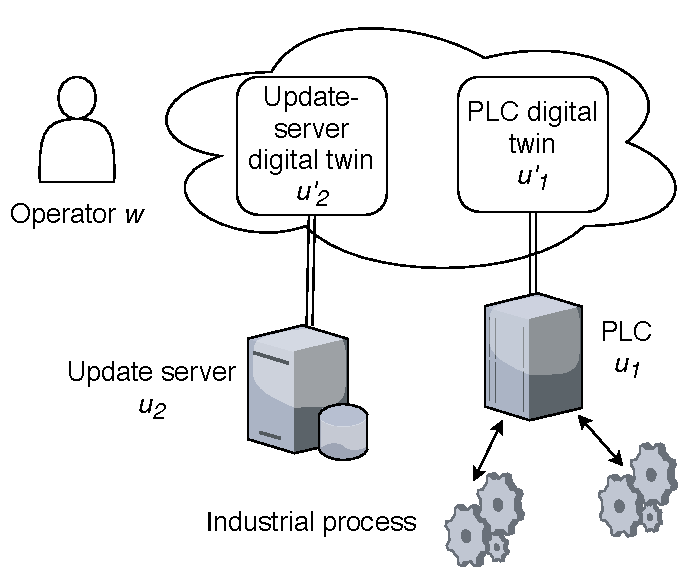
\includegraphics[scale=0.5]{papers/digital-twin/images/FIG7_TII-19-1326}
    \caption{Setup of out digital twin and software update scenario.}
    \label{figure:setup}
\end{figure}

The state information for the supported twins are selected to be: $s_{u'_1} =$ \texttt{[ctrl\_flag, ctrl\_url, sw\_state]} and  $s_{u'_2} = $ \texttt{[ctrl\_url, sw\_package]}\footnote{Here is actually no state information with origin from the physical twin, $u_2$, but just digital twin state information which is propagated to the physical twin.}.  \texttt{ctrl\_flag} is a value holding software upgrade request control and error information and the \texttt{ctrl\_url} is a URL of a new software package to be installed. \texttt{sw\_state} is a list of all current software packages and versions installed on a unit and \texttt{sw\_package} is a new software package.  We also assumes a remote operator, $w$, to be present in the system controlling software upgrades through a remote user device over standard internet. 


\subsection{PLC software update process}
$w$ identifies a new software package, $q$, and connects to the external server $u'_2$.  $w$ then downloads $q$ to $u'_2$ and $w$  receives a \texttt{ctrl\_url} value for the package in return. $u'_2$ then updates the state $\hat{s}_{u'_2,0}$ to reflect the storage of the new software package. Then a synchronization takes place between $u'_2$ and $u_2$. The synchronization is done by sending $\Delta_{\hat{s}_{u'_2}} = $ \texttt{ctrl\_url}$+ q$ from $u'_2$ to $u_2$. This in turn, triggers $u_2$ through the functions $h_{u_2}$ and $z_{u_2}$, to update its internal state, resulting in the storage of $q$ which can be downloaded from \texttt{ctrl\_url} to other units within the local factory network. 

$w$ makes a second request using the newly received \texttt{ctrl\_url} and with information regarding the new software packages towards $u'_1$. The request trigger $u'_1$ to update states $s_{u'_1,1}$: \texttt{ctrl\_flag}, \texttt{ctrl\_url}, \texttt{sw\_state}, where \texttt{ctrl\_flag} contains ''available software update indicator'', \texttt{ctrl\_url} contains the URL to the new software package on $u_2$ and \texttt{sw\_state} contains version information for the pending new software. In the clock cycle 2, this information is propagated to $u_1$ through  $\Delta_{\hat{s}_{u'_1}}$. This values in combination with the functions $h_{u_1}$ and $z_{u_1}$ give an updated state $s_{u_1,2}$.
The SW update flag in state $s_{u_1,2}$ triggers $u_1$ to set the state to update pending allowing to $u_2$ using \texttt{ctrl\_url} to download and install the new SW package, $q$. Once, the update is finalized, the update status information as well as the new SW state information is propagated back to $u'_1$ through updates of the \texttt{ctrl\_flag} and \texttt{sw\_state}.

\vspace*{-0.15in}
\subsection{Performance evaluation}
We have implemented the scenario, described above, with a SW update process using digital twins. As the PLC $u_1$ we have used OpenPLC\cite{Alvares2014}, a free, open source PLC implementation, running on a RaspberryPI\footnote{https://www.raspberrypi.org }. The Raspberry Pi we have used is a model 2 v1.1 with an ARM Cortex-A7 quad-core processor, clocked at 900MHz.

The digital twins $u'_1, u'_2$ are running as separate processes in a Ubuntu 18.04 desktop host. The same host also functions as the update server $u_2$. Since the physical entities synchronize with digital-twins outside the protected factory network the synchronization protocol is secured by DLTS. 

\subsubsection{Update time depending on synchronization frequency}
In order to evaluate the state synchronization protocol we have looked at the SW update scenario. We want to examine how the state synchronization process affects other processes running on the system.

First we ran tests without state synchronization to establish a base line for how long time the update process takes. Then we ran the SW update process with state synchronization at different frequencies. We evaluated performance at 1, 10 and 100 state synchronizations per second. The result can be seen in Fig. \ref{figure:times}\footnote{In the simple system we are using, actually, the state exchange can be omitted in most cases as we very seldom have state changes, but in our evaluation, we anyway forced a state exchange to take place in order to test the synchronization frequency performance impact.}.

As can be seen from the figure the performance impact of the state synchronization is very small. Only at a large number of synchronizations per second is the performance noticeable.
\begin{figure}[ht]
\vspace*{-0.2in}
   \centering
    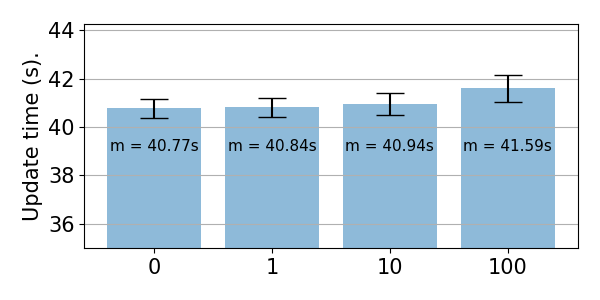
\includegraphics[height=4cm, width=7cm]{papers/digital-twin/images/FIG8_TII-19-1326}
    \vspace*{-0.15in}
    \caption{Update times when using state synchronization at different frequencies.}
    \label{figure:times}
\end{figure}

\subsubsection{Compassion of DTLS Cipher Suites}
We have compared different DLTS cipher suites to evaluate if this impacts performance. The default strong suite AES-256-GCM with SHA384 was compared to the weaker AES-128-GCM with SHA256. The results can be seen in Figure \ref{figure:ciphers}. It can be noted that the choice of ciphers has only a very small impact on the performance of the update process.

\begin{figure}[ht]
\vspace*{-0.2in}
   \centering
    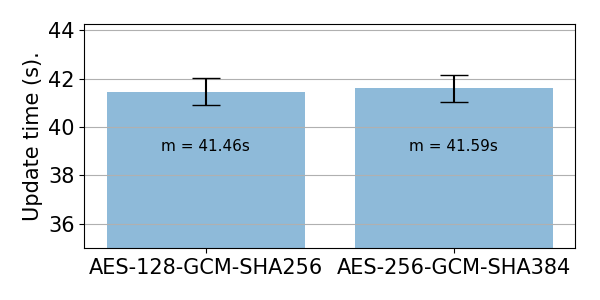
\includegraphics[height=4cm, width=7cm]{papers/digital-twin/images/FIG9_TII-19-1326}
    \vspace*{-0.15in}
    \caption{Comparison of update times with different DTLS cipher-suites.}
    \label{figure:ciphers}
\end{figure}

\subsubsection{Computation cost}
A PLC is not a constrained device in a traditional sense, however, since it controls a time-critical process CPU-time is limited. Any added features must consider this so time-critical deadlines are kept.

We have measured the CPU-time needed by the PLC to implement our state synchronization protocol. By running the protocol over an extended time we have come to the following numbers as seen in Table \ref{table:cpu-time}. 

As shown in the table the CPU-time needed by the PLC to implement the state synchronization protocol is very small. An even slower CPU will still be able to run the state synchronization without overloading the processor.

\begin{table}[]
\begin{tabular}{lll}

 \thead{CPU-time (ms)\\per synchronization} & \thead{ CPU-load  \\ 10 synchronizations/s} & \thead{CPU-load \\ 100 synchronizations/s} \\ \hline
           $0.3772 \: (s = 0.0602)$   & $0.0038\%$   &   $0.0377\%$                       \\ 
\end{tabular}
\caption{Measurements of CPU-time per state synchronization message and CPU-load.}
\label{table:cpu-time}
\end{table}
% 900mhz 4 cors  



\subsubsection{Network performance}
Evaluating network performance for the state synchronization process is difficult to do without real ICS network traffic to base an evaluation scenario on. Hence, instead we evaluated the performance in an isolated system. We measured the bandwidth consumption for the PLC during the update process. We then measured the bandwidth for the update process while synchronizing with the PLC's digital-twin. The synchronization messages were of size 22 bytes in each direction. The bandwidth consumption can be seen in Table \ref{table:network-overhead}. As can be seen from the Table the bandwidth consumption is reasonable for small synchronization frequencies.

\begin{table}[]
\begin{tabular}{l|l|l}
    & Bandwidth to PLC & Bandwidth from PLC \\ \hline
No synch  &     0.97 KB/s      &     2.06 KB/s    \\
1 synch/s &     1.20 KB/s       &    2.38 KB/s   \\
10 synch/s &      2.16 KB/s     &     3.35 KB/s        \\
100 synch/s &     10.88 KB/s     &    12.06 KB/s

\end{tabular}
\caption{Bandwidth to and from the PLC when updating.}
\label{table:network-overhead}
\end{table}


\iffalse
\begin{table}[]
\begin{tabular}{l|l|lll}
    Message Length & Synchronization  & \multicolumn{3}{l}{Devices on network} \\
                                &  frequency                                   & 1           & 10         & 100         \\ \hline
\multirow{3}{*}{20}             & 1                                   & 40B/s       & 400B/s     & 4KB/s       \\
                                & 10                                  & 400B/s      & 4KB/s      & 40KB/s      \\
                                & 30                                  & 600B/s      & 6KB/S      & 60KB/s      \\
\multirow{3}{*}{50}             & 1                                   & 100B/s      & 1KB/s      & 10KB/s      \\
                                & 10                                  & 1KB/s       & 10KB/s     & 100KB/s     \\
                                & 30                                  & 3KB/s       & 30KB/s     & 300KB/s    
\end{tabular}
\caption{Network usage for different sizes of synchronization messages, synchronization frequencies and number of devices on network.}
\label{table:network-overhead}
\end{table}
\fi

\section{Conclusion and future work}
\label{sec:digital-twin:conclusion}
Motivated by the need for new security models and principles in IACS to open up the systems for cloud based processing and data sharing, we investigated how digital twins can work as a security enablers in IACS. We introduced a new adversary model, made basic security definitions, identified security requirements, made a novel security architecture and in particular state replication design for a digital twin based IACS. The new state replication design as well as the architecture were then security evaluated against the identified requirements. We showed that the proposed synchronization design meets the introduced digital twin synchronization requirements. Furthermore, we made a high-level design of the other security components in the architecture and argue about how the suggested functions will help in meeting the identified security requirements.  Through our proof of concept implementation and performance evaluation, we also showed that the new digital twin synchronization model works well in practice for a small but real production case with reasonable performance impact. Especially, we show that as long as we have not too high update frequency, the performance impact on a platform like RaspberryPI is negligible. As expected, the bandwidth increases linear with the synchronization frequency. In our evaluation, we only reflected a few PLC states, and obviously, the more fine grain states that are reflected, the more impact it will have on the system performance and bandwidth consumption.

The results shows that a digital twin based security architecture can be a promising way to protect IACS while open them up for external data sharing and access. We have here worked with defining a suitable overall architecture and synchronization model. In order to develop a fully working system based on our architecture and approach, more work is needed. Below, we discuss the most important future work:
\begin{itemize}
\item \textbf{Performance:} We have here made first proof of concept of the architecture. In order to see the effect of the architecture on different platform and production scenarios, more performance evaluations on different platform, with more complex digital twin state models and with larger amount of production nodes are needed. 
\item \textbf{Intrusion detection:} In our security architecture, we have only show how on principle level how  to integrate intrusion detection at the boarder to the virtual domain. It is left for future research to design and integrate intrusion detection in a fully working system.
\item \textbf{Access control:} The architecture allows for advanced access control in the virtual domain. The main advantage with this approach is that this can be supported without affecting the production domain at all. It remains to design and evaluate this approach in a full system implementation of the architecture.
\item\textbf{Formal security analysis:} We have proven the consistency of the proposed synchronization protocol and showed that the security of the protocol depends on the security of the underlying used secure channel. Formal analysis of the security of the complete system design and all protocols are left for future work. 
\item \textbf{Security analysis services:} Apart from IDS and access control enforcement in the virtual domain, additional security analysis services may be supported as virtual components as we showed in our architecture design. This include services such as virus scan, DoS prevention etc. The design and evaluation of such services is left to future research as well.
\end{itemize}

\section*{Acknowledgement}
We would like to thank the SSF SEC4FACTORY project team for valuable discussions regarding the research direction and results presented in the paper. In particular we would like to thank the TetraPak project members for their valuable feedback and suggestions.

{\raggedright
        \printbibliography[segment=\therefsegment,heading=subbibliography]
}


\fi

\part[Popular Science Summary in Swedish]{\texorpdfstring{%
Popular Science Summary\\in Swedish}{%
Popular Science Summary in Swedish}}

% (the following ends the \ifcontributionStatementOnly a loooong time ago in this file)
\fi

% (the following ends the \ifpopvetOnly a loooong time ago in this file)
\fi

\makeatletter
\def\@makeschapterhead#1{%
  \vspace*{10\p@}%
  {\parindent \z@ \raggedleft \reset@font
            \sffamily \bfseries \vphantom{\@chapapp{} \thechapter}
        \par\nobreak
        \interlinepenalty\@M
    \Huge  #1\par\nobreak
    \hrulefill
    \par\nobreak
    \vskip 16\p@
  }}
\makeatother

\fancyhead[RE,LO]{Populärvetenskaplig sammanfattning}
TODO


\end{document}

